\documentclass{book}

\usepackage{geometry}
\usepackage{graphicx}
\usepackage{float}
\usepackage{makeidx}
\usepackage{tabularx}
\usepackage{subcaption}

\geometry{letterpaper}

\makeindex

\title{Williams Trading Manual}

\author{\copyright~Copyright 2016, Williams Trading Co.\\
 All rights reserved.}

\date{July 29, 2016}

\begin{document}
	
\maketitle

\clearpage
\pagenumbering{roman}
\addcontentsline{toc}{section}{Table of Contents}
\tableofcontents

\setlength{\parindent}{0pt}
\setlength{\parskip}{1em}

\clearpage
\pagenumbering{arabic}
\chapter{Introduction}
\section{Introduction}

Welcome to The Williams Trading Company and its Affiliates!

Starting a new job is exciting, but at times can be overwhelming. This Employee Handbook has been developed to help you become acquainted with our company and answer many of your initial questions.

As an employee of The Williams Trading Company and its Affiliates, you are very important. Your contribution cannot be overstated. Our goal is to provide the finest-quality products and services to our customers and to do so more efficiently and economically than our competitors. By satisfying our customers' needs, we ensure they will continue to do business with us and will recommend us to others.

You are an important part of this process because your work directly influences our company's reputation.

We are glad you have joined us, and we hope you will find your work to be both challenging and rewarding.
\\
\\
Sincerely,
\\
\\
Robert Pyne, Jr.\\
President
\chapter{Handbook}
\section{The Way We Work}

\subsection{A Word About This Handbook}

This Employee Handbook contains information about the employment policies and practices of the company. We expect each employee to read this Employee Handbook carefully, as it is a valuable reference for understanding your job and the company. The policies outlined in this Employee Handbook should be regarded as management guidelines only, which in a developing business will require changes from time to time. The company retains the right to make decisions involving employment as needed in order to conduct its work in a manner that is beneficial to the employees and the company. This Employee Handbook supersedes and replaces any and all prior Employee Handbooks and any inconsistent verbal or written policy statements.

Except for the policy of at-will employment, which can only be changed by the President of the company in a sidnged written contract, the company reserves the right to revise, delete and add to the provisions of this Employee Handbook at any time without further notice. All such revisions, deletions or additions to the Employee Handbook must be in writing and must be signed by the President of the company. No oral statements or representations can change the provisions of this Employee Handbook.

The provisions of this Employee Handbook are not intended to create contractual obligations with respect to any matters it covers. Nor is this Employee Handbook intended to create a contract guaranteeing that you will be employed for any specific time period.

\textbf{OUR COMPANY IS AN AT-WILL EMPLOYER, THIS MEANS THAT REGARDLESS OF ANY PROVISION IN THIS EMPLOYEE HANDBOOK, EITHER YOU OR THE COMPANY MAY TERMINATE THE EMPLOYMENT RELATIONSHIP AT ANY TIME, FOR ANY REASON, WITH OR WITHOUT CAUSE OR NOTICE. NOTHING IN THIS EMPLOYEE HANDBOOK OR IN ANY DOCUMENT OR STATEMENT, WRITTEN OR ORAL, SHALL LIMIT THE RIGHT TO TERMINATE EMPLOYMENT AT-WILL. NO OFFICER, EMPLOYEE OR REPRESENTATIVE OF THE COMPANY IS AUTHORIZED TO ENTER INTO AN AGREEMENT, EXPRESSED OR IMPLIED, WITH ANY EMPLOYEE FOR EMPLOYMENT FOR A SPECIFIED PERIOD OF TIME UNLESS SUCH AN AGREEMENT IS IN A WRITTEN CONTRACT SIGNED BY THE PRESIDENT OF THE COMPANY.}

This employee Handbook refers to current benefit plans maintained by the company. Refer to the actual plan documents and summary plan descriptions if you have specific questions regarding the benefit plan. those documents are controlling.

Likewise, if a written contract is inconsistent with the Employee Handbook, the written contract is controlling.

\subsection{Equal Employment Opportunity}

Our company is committed to equal employment opportunity. We will not discriminate against employees or applicants for employment on any legally-recognized basis ["protected class"] including, but not limited to: veteran status, uniform service member status, race, color, religion, sex, national origin, age, physical or mental disability or any other protected class under federal, state or local law.

In New Jersey, the following are a protected class: race, creed, color, national origin, ancestry, age, marital status, domestic partnership status, civil union status, affectional or sexual orientation, gender identity or expression, genetic information, sex, atypical hereditary cellular or blood traits, nationality, refusing to submit to a genetic test or make available the results of a genetic test to an employer, disability, liability for service in the U.S. military, and religious practice or observance.

You may discuss equal employment opportunity related questions with the controller or any other member of management.

\subsection{Americans with Disabilities Act}

Our company is committed to providing equal employment opportunities to qualified individuals with disabilities. This may include providing reasonable accommodation where appropriate in order for an otherwise qualified individual to perform the essential functions of the job. It is your responsibility to notify the controller of the need for accommodation. Upon doing so the controller may ask you for your input or the type of accommodation you believe may be necessary or the functional limitations caused by your disability. Also, when appropriate, we may need your permission to obtain additional information from your physician or other medical or rehabilitation professionals.

\subsection{A Word About our Employee Relations Philosophy}

We are committed to providing the best possible climate for maximum development and goal achievement for all employees. Our practice is to treat each employee as an individual. We seek to develop a spirit of teamwork; individuals working together to attain a common goal.

In order to maintain an atmosphere where these goals can be accomplished, we provide a comfortable and progressive workplace. Most importantly, we have a workplace where communication is open an problems can be discussed and resolved in a mutually respectful atmosphere. We take into account individual circumstances and the individual employee.

We firmly believe that with direct communication, we can continue to resolve any difficulties that may arise and develop a mutually beneficial relationship.

\subsection{Non-Harassment}

We prohibit harassment of one employee by another employee, manager or third party for any reason including, but not limited to: veteran status, race, color, religion, sex, national origin, age and physical or mental disability. Harassment of third parties by our employees is also prohibited.

Race, creed, color, national origin, ancestry, age, marital status, domestic partnership status, affectional or sexual orientation, genetic information, sex, atypical hereditary cellular or blood trait, nationality, refusing to submit to a genetic test or make available the results of a genetic test to an employer, disability and liability for service in the U.S. military are protected classes in New Jersey.

The purpose of this policy is not to regulate the personal morality of employees. it is to assure that in the workplace, no employee harasses another for any reason.

While it is not easy to define precisely what harassment is, it includes: slurs, epithets, threats, derogatory comments or visual depictions, unwelcome jokes and teasing.

Any employee who feels that (s)he is a victim of such harassment should immediately report the matter to the controller or any other member of management. The company will investigate all such reports as confidentially as possible. Adverse action will not be taken against an employee because he or she, in good faith, reports or participates in the investigation of a violation of this policy. Violations of this policy are not permitted and may result in disciplinary action, up to and including discharge.

\subsection{Sexual Harassment}

Sexual harassment is against company policy and is unlawful under state and federal law.

We firmly prohibit sexual harassment of any employee by another employee, manager or third party. Harassment of third parties by our employees is also prohibited. The purpose of this policy is not to regulate the morality of employees. It is to assure that in the workplace, no employee is subject to sexual harassment. While it is not easy to define precisely what sexual harassment is, it may include: unwelcome sexual advances, requests for sexual favors and/or verbal or physical conduct of a sexual nature including, but not limited to: sexually-related drawings, pictures, jokes, teasing, uninvited touching or other sexually-related comments.

Sexual harassment of an employee will not be tolerated. Violations of this policy may result in disciplinary action, up to and including discharge. There will be no adverse action taken against employees who, in good faith, report violations of this policy or participate in the investigation of such violations.

Any employee who feels that (s)he is a victim of sexual harassment should immediately report such actions in accordance with the following procedure. All complaints will be promptly and thoroughly investigated as confidentially as possible.

Any employee who believes that (s)he is a victim of sexual harassment or has been retaliated against for complaining of sexual harassment, should report the act immediately to the manager. If you prefer not to discuss the matter with the manager, you may contact any other member of management.

The company will investigate every reported incident immediately. Any employee, manager or agent of the company who has been found to have violated this policy may be subject to appropriate disciplinary action, up to and including immediate discharge.

The company will conduct all investigations in a discreet manner. The company recognizes that every investigation requires a determination based on all the facts in the matter. We also recognize the serious impact a false accusation can have. We trust that employees will continue to act responsibly.

The reporting employee and any employee participating in any investigation under this policy have the company's assurance that no reprisals will be taken as a result of a sexual harassment complaint. it is our policy to encourage discussion of the matter, to help protect others from being subjected to similar inappropriate behavior.

\subsection{Categories of Employment}

INTRODUCTORY PERIOD: Full-time and part-time employees are on an introductory period during their first 90 days of employment.

During this time, you will be able to determine if your new job is suitable for you and your manager will have an opportunity to evaluate your work performance. However, the completion of the introductory period does not guarantee employment for any period of time since you are an at-will employee both during and after your introductory period.

FULL-TIME EMPLOYEES regularly work at least a 40-hour workweek.

PART-TIME EMPLOYEES work less than 28 hours each week.

SEASONAL EMPLOYEES perform a job for a specified time, normally less than one year.

In addition to the preceding categories, employees are also categorized as "exempt" or "non-exempt."

NON-EXEMPT EMPLOYEES are entitled to overtime pay as required by applicable federal and state law.

EXEMPT EMPLOYEES are not entitled to overtime pay and may also be exempt from minimum wage requirements pursuant.to applicable federal and state laws.

Upon hire, your manager will notify you of your employment classification.

\subsection{New Employee Orientation}

Upon joining our company, you were given this copy of our Employee Handbook. After reading this Employee Handbook please sign the receipt page and return it to your manager. You will be asked to complete personnel, payroll and benefit forms.

If you lose your Employee Handbook or if it becomes damaged in any way, please notify your manager as soon as possible to obtain a replacement copy.

Your manager is responsible for the operations of your department. (S)he is a good source of information about the company and your job.

\subsection{Immigration Reform and Control Act}

in compliance with the federal Immigration Reform and Control Act of 1986 (IRCA), as amended, and any state law requirements, if applicable, our company is committed to employing only individuals who are authorized to work in the United States.

Each new employee, as a condition of employment, must complete the Employment Eligibility Verification Form I-9 and present documentation establishing identity and employment eligibility. 

if an employee is authorized to work in this country for a limited time period, the individual will be required to submit proof of renewed employment eligibility prior to expiration of that period to remain employed by the company.

\subsection{Suggestions and Ideas}

We are always interested in your constructive ideas and suggestions for improving our operations. Your suggestions should be submitted in writing or email to the president.

After we investigate your suggestion, you will be notified whether it is feasible to be put into practice.

We believe that suggestions indicate initiative. With your approval, we will place the written suggestion in your personnel file and consider it at the time of your performance review.

\subsection{Talk to Us}

We encourage you to bring your questions, suggestions and complaints to our attention. We will carefully consider each of these in our continuing effort to improve operations.

If you feel you have a problem, present the situation to your manager so that the problem can be settled by examination and discussion of the facts. We hope that your manager is able to satisfactorily resolve most matters.

If you still have questions after meeting with your manager or if you would like further clarification on the matter, request a meeting with the controller. (S)he will review the issues and meet with you to discuss possible solutions.

Finally, if you still believe that your problem has not been fairly or fully addressed, request a meeting with the President.

Your suggestions and comments on any subject are important, and we encourage you to take every opportunity to discuss them with us. Your job will not be adversely affected in any way because you choose to use this procedure.

if at any time you do not feel comfortable speaking with your manager or the next level of management, discuss your concern with any other member of management with whom you feel comfortable.

\section{Your Pay and Progress}

\subsection{Recording Your Time}

Non-exempt employees must record their hours on a time clock. Use the hand-punch at the beginning and end of your shift. Do not use the hand-punch more than five minutes before the beginning or after the end of your shift. You are expected to work until the end of your shift. 

All employees subject to this policy are required to accurately record all time worked.

The workweek starts on Sunday and ends on Saturday.

\subsection{Payday}

You will be paid biweekly on Friday for the 2 week period which ends on the previous Saturday. If a payday falls on a nonworking day, employees will be paid the preceding workday.

Checks will be distributed by management prior to the end of your shift.

Please review your paycheck for errors. if you find a mistake, report it to your manager immediately. Your manager will assist you in taking the steps necessary to correct the error.

\subsection{Authorized Check Pick-Up}

If an employee is absent on pay day and instructs someone to pick up his or her paycheck, a note signed by the employee authorizing the release of the pay check to the specific person must be provided before the check may be released. The person picking up the pay check must show proper identification and sign for receipt of the check. This policy is intended to protect both the employee and the Company. Any terminated employee will have their final paychecks mailed to them. No exceptions.

\subsection{Paycheck Deductions}

The company is required by law to make certain deductions from your paycheck each pay period. Such deductions typically include federal and state taxes and Social Security (FICA) taxes. Depending on the state in which you are employed and the benefits you choose, there may be additional deductions. All deductions and the amount of the deductions are listed on your pay stub. These deductions are totaled each year for you on your Form W-2, Wage and Tax Statement.

If is the policy of the company that exempt (salaried) employees‘ pay will not be “docked,” or subject to deductions, in violation of salary pay rules issued by the United States Department of Labor and any corresponding rules issued by the state government, as applicable. However, the company may make deductions from employees‘ salaries in a way that is permitted under federal and state wage and hour rules. Employees will be reimbursed in full for any isolated, inadvertent, or improper deductions, as defined by law.

Thus, exempt employees may be subject to the following salary deductions, except where prohibited by state law, but only for the following reasons:

\begin{itemize} 	
	\item Absences of one or more full days for personal 	reasons, other than sickness or disability; or 	
	\item Absences of one or more full days due to 	sickness or disability, if there is a plan, policy, or 	practice providing replacement compensation for 	such absences; or ,	 
	\item Absences of one or more full days before 	eligibility under such a plan, policy, or practice or 	after replacement compensation for such 	absences has been exhausted; or 	
	\item Suspensions of one or more full days for 	violations of safety rules of major significance; or 	
	\item Suspensions of one or more full days for 	violations of written workplace conduct rules, 	such as rules against sexual harassment and 	workplace violence; or 	
	\item Payment of actual time worked in the first and 	last weeks of employment, resulting in a 	proportional rate of an employee's full salary; or 	
	\item Any unpaid leave taken under the Family and 	Medical Leave Act; or	 	
	\item Negative paid-time—off balances, in whole-day 	increments only. 
\end{itemize}

lf questions or concerns about any pay deductions arise, employees may discuss and resolve them with the Human Resources Department.

\subsection{Garnishment/Child Support}

When an employee's wages are garnished by a court order, our company is legally bound to withhold the amount indicated in the garnishment order from the employee's paycheck. Our company will, however, honor applicable federal and state guidelines that protect a certain amount of an employee's income from being subject to garnishment.

\subsection{Direct Deposit}

You have the option of receiving your pay in a payroll check or having your pay deposited into your bank account through our direct deposit program.

\subsection{Performance Reviews}

Your performance is important to our company. Once each year, on or about your anniversary date, your manager and the President will review your job progress within our company and help you to set new job performance plans.

Our performance review program provides the basis for better understanding between you and your manager and the President, with respect to your job performance, potential and development within the company. A pay increase may or may not be associated with the performance review, dependent upon the overall performance of the individual and of the Company as a whole.

New employees will generally be reviewed at the end of their introductory period.

\subsection{Pay Advances}

Pay advances will not be granted to employees.

\subsection{Overtime}

There may be times when you will need to work overtime so that we may meet the needs of our customers. Although you will be given advance notice when feasible, this is not always possible. Non-exempt employees must have all overtime approved in advance by the managers.

Non-exempt employees will be paid at a rate of time and one-half their regular hourly rate for hours worked in excess of 40 hours in a workweek, unless state law provides otherwise.

Only actual hours worked and holiday hours count toward computing weekly overtime.

If you have any questions concerning overtime pay, check with the managers.

\subsection{Shift Premiums}

A premium rate is paid to employees who work the night shift in accordance with state and federal wage and hour laws.

\section{Time Away From Work and Other Benefits}

\subsection{Employee Benefits}

Our company has developed a comprehensive set of employee benefit programs to supplement our employees‘ regular wages. Our benefits represent a hidden value of additional income to our employees.

This Employee Handbook describes the current benefit plans maintained by the company. Refer to the actual plan documents and summary plan descriptions if you have specific questions regarding the benefit plan. Those documents are controlling.

The company reserves the right to modify its benefits at any time. We will keep you informed of any changes.

\subsection{Holidays}

Our company normally observes the following holidays during the year:

New Year's Day, Memorial Day, Independence Day, Labor Day, Thanksgiving Day, Christmas Day

If one of the above holidays falls on Saturday, it normally is observed on the preceding Friday. If one falls on Sunday, it normally is observed on the following Monday.

Eligible employees receive a paid holiday only if the holiday falls on a day they are normally scheduled to work.

Full-time employees are eligible for paid holidays after completing their introductory period.

Exempt employees will receive holiday pay in compliance with state and federal wage and hour laws.

Non-exempt employees must work their scheduled work day before and after the holiday in order to be paid for the holiday, unless they have utilized an eligible sick and/or vacation day with two weeks’ advance notice.

\subsection{Vacation - Warehouse Employees}

Full-time, warehouse employees are eligible for paid vacation time.

Vacation is calculated according to the anniversary year.

After the completion of your initial year of employment, you are entitled to five (5) days vacation.

After completion of your 5th year, you are entitled to ten (10) days of paid vacation.

Submit vacation requests in writing at least 30 days in advance to your manager or manager. When possible, vacation requests are granted, taking into account operating requirements. Length of employment may determine priority in scheduling vacation times.

Vacation can not be carried over from one year to the next nor is vacation pay granted in lieu of taking the actual time off.

Vacation should be taken in blocks of four or eight hours at a time.

At the discretion of management, sick and/or vacation must be utilized when taking time off from work.

Eligible employees who provide at least two weeks‘ advance notice of their resignation will be paid for accrued but unused vacation, unless state law dictates otherwise. If advance notice of resignation is not given, the employee will not be paid for accrued but unused vacation upon resignation.

\subsection{Vacation - Managers and Office Employees}

Full-time, office employees are eligible for paid vacation time.

Vacation is calculated according to the anniversary year.

After completion of your initial year of employment, you are entitled to five (5) vacation days. Thereafter, you receive vacation as follows:

After completion of your 2nd year, you are entitled to ten (10) days of paid vacation annually.

After completion of your 5th year, you are entitled to fifteen (15) days of paid vacation annually.

After completion of your 20th year, you are entitled to twenty (20) days of paid vacation annually.

Submit vacation requests in writing at least 30 days in advance to your manager or manager. When possible, vacation requests are granted, taking into account operating requirements. Length of employment may determine priority in scheduling vacation times.

Vacation can not be carried over from one year to the

next nor is vacation pay granted in lieu of taking the actual time off.

Vacation should be taken in blocks of four or eight hours at a time.

Eligible employees who provide at least two weeks’ advance notice of their resignation will be paid for accrued but unused vacation, unless state law dictates otherwise. If advance notice of resignation is not given, the employee will not be paid for accrued but unused vacation upon resignation.

\subsection{Sick/Personal Days}

Full-time employees are eligible, after completing their introductory period, for two paid sick days each year: one (1) day to be used during the first six months of the year, and one (1) day to be used during the second six months of the year.

Exempt employees will receive sick pay in compliance with state and federal wage and hour laws.

You may use accrued sick time to care for a child who is sick.

Sick days cannot be carried over to the following year. Employees are not paid in lieu of taking the actual time off.

Employees are not paid for earned but unused sick days upon termination.

\subsection{Jury Duty}

Full-time employees who have completed their introductory period are eligible for one (1) paid day in order to serve when they are summoned for jury duty. Thereafter, employees are granted unpaid leave. Part- time employees and those employees who have not completed their introductory period may take unpaid time off in order to serve. Employees must provide proof of their service to their manager.

Exempt employees may be provided time off with pay when necessary to comply with state and federal wage and hour laws.

Make arrangements with your manager as soon as you receive your summons.

We expect you to return to your job if you are excused from jury duty during your regular working hours.

\subsection{Military Leave}

Employees who are required to fulfill military obligations in any branch of the Armed Forces of the United States or in state military service will be given the necessary time off and reinstated in accordance with federal and state law.

The time off will be unpaid, except where state law dictates otherwise. Exempt employees may be provided time off with pay when necessary to comply with state and federal wage and hour laws.

Accrued vacation may be used for this leave if the employee chooses. Military orders should be presented to the controller and arrangements for leave made as early as possible before departure. Employees are required to give advance notice of their service obligations to the company unless military necessity makes this impossible. You must notify the controller of your intent to return to employment based on requirements of the law. Your benefits may continue to accrue during the period of leave in accordance with state and federal law.

Additional information regarding military leaves may be obtained from the controller.

\subsection{Bereavement Leave}

Full-time employees who have completed their introductory period are eligible for two paid days for the death of an immediate family member. Members of the immediate family include spouses, parents, brothers, sisters, children, grandchildren, grandparents, and parents-in-law.

Requests for bereavement leave should be made to your immediate manager as soon as possible, and documentation regarding your relationship and attendance may be requested.

\subsection{Medical Insurance}

Eligible full-time employees may enroll in an employee, an employee plus spouse, an employee plus child, or a family contract on the first of the month after completing 90 days of employment.

information and enrollment forms may be obtained from the controller.

To assist you with the cost of this insurance, our company pays a portion of an employee, an employee plus spouse, employee plus child, or a family contract. You are responsible for paying the balance through payroll deduction.

Participating employees are also covered under our medical insurance plan's prescription drug program.

A booklet containing the details of the plan and eligibility requirements may be obtained from the controller.

Refer to the actual plan document and summary plan description if you have specific questions regarding this benefit plan. Those documents are controlling.

Upon termination you may be entitled to continuation or conversion of the group medical insurance plan in accordance with the terms of the policy and/or applicable state and federal law. For more information contact the controller.

\subsection{Dental Insurance}

Eligible full-time employees may enroll in an employee, employee plus spouse, employee plus child, or a family contract after completing 90 days of employment.

Information and enrollment forms may be obtained from the controller.

Our company pays the full cost of an employee contract. If you elect dependent coverage, you are responsible for paying the difference through payroll deduction.

A booklet containing the details of the plan and the eligibility requirements may be obtained from the controller.

Refer to the actual plan document and summary plan description if you have specific questions regarding this benefit plan. Those documents are controlling.

Upon termination you may be entitled to continuation or conversion of the group dental insurance plan in accordance with the terms of the policy and/or applicable state and federal law. For more information contact the controller.

\subsection{COBRA}

You and your covered dependents will have the opportunity to continue medical and/or dental benefits for a period of up to 36 months under the provisions of the Consolidated Omnibus Budget Reconciliation Act (COBRA) when group medical and/or dental coverage for you and your covered dependents would otherwise end due to your death or because:

\begin{itemize} 	\item your employment terminates, for a reason other 	than gross misconduct; or
	
	\item your employment status changes due to a 	reduction in hours; or
	
	\item your child ceases to be a "dependent child" 	under the terms of the medical and/or dental 	plan; or
	
	\item you become divorced or legally separated; or
	
	\item you become entitled to Medicare. \end{itemize}

in the event of divorce, legal separation, or a child's loss of dependent status, you or a family member must notify the plan administrator within 60 days of the occurrence of the event.

The plan administrator will notify the individuals eligible for continuation coverage of their right to elect COBRA continuation coverage.

For more information regarding COBRA, you may contact the controller.

\subsection{Life Insurance}

Eligible full-time employees may enroll in this plan after 90 days of employment.

You must complete an insurance form and designate your beneficiary.

The cost of this insurance is fully paid by the company.

Participating employees may also be covered under the plan's Accidental Death and Dismemberment rider.

You also have the option of purchasing additional insurance through our group plan.

Complete details of this plan may be obtained from the controller.

\subsection{Section 125 Plans}

Our company offers a pretax benefits contribution option for employees. This employee benefit is known as a Section 125 plan.

A Section 125 plan is a benefit plan that allows you to make contributions toward . premiums for medical insurance and dental insurance on a "before tax", rather than an "after tax" basis. Your premium contributions are deducted from your gross pay before income tax and Social Security is calculated.

To participate in this plan, complete an election form and return it to the controller.

You cannot make any changes to your medical insurance and dental insurance coverage until the next open enrollment period, unless your family status changes or you become eligible for a special enrollment period due to a loss of coverage. Family status changes include marriage, divorce, death of a spouse or child, birth or adoption of a child or termination of employment of your spouse. A change in election due to a change in family status is effective the next pay period.

\subsection{Disability Leave}

Full-time and part-time employees are eligible for an unpaid disability leave immediately upon hire. Disability leave due to non-occupational illness, injury or pregnancy-related disability is not to exceed 12 weeks.

Granting this leave prior to the completion of the eligibility period and/or beyond the maximum period as stated above may be required as a reasonable accommodation to an employee in accordance with the Americans with Disabilities Act.

Employees requesting leave must provide written notice of the disability, including a doctor's certificate stating the nature of the disability and the expected date of return to work.

You may continue your medical insurance and dental insurance coverage by making arrangements with the controller to pay the entire monthly premium in advance each month.

When you are able to return to work, give us at least one to two week's advance written notice. include a doctor's certificate stating that you are medically able to return to your normal duties.

We will return you to the same or similar position you held prior to the disability leave, subject to our staffing and business requirements. Your continued absence from work beyond your disability, as determined by your physician, will be deemed a voluntary termination of your employment.

This leave may run concurrently with the Federal Family and Medical Leave Act and/or any other leave where permitted by state and federal law.

\subsection{Federal Family and Medical Leave Act}

The Family and Medical Leave Act (“FMLA”) provides eligible employees the opportunity to take unpaid job- protected leave for certain specific reasons. The maximum amount of leave an employee may use is either 12 or 26 weeks within a 12-month period depending on the reasons for the leave.

\subsubsection{Employee Eligibility}

To be eligible for FMLA leave, you must:

\begin{enumerate} 	\item have worked at least 12 months for the company 	in the preceding seven years (limited exception 	apply to the seven-year requirement;
	
	\item have worked at least 1,250 hours for the 	company over the preceding 12 months;
	
	and
	
	\item currently work at a location where there are at 	least 50 employees within 75 miles. \end{enumerate}

\subsubsection{Conditions Triggering Leave}

FMLA leave may be taken for the following reasons:

\begin{enumerate} 	\item birth of a child, or to care for a newly-born child 	(up to 12 weeks);
	
	\item placement of a child with the employee for 	adoption or foster care (up to 12 weeks);
	
	\item to care for an immediate family member 	(employee's spouse, child, or parent) with a 	serioushealth condition (up to 12 weeks);
	
	\item because of the employee's serious health 	condition that makes the employee unable to 	perform the employee's job (up to 12 weeks);
	
	\item to care for a covered servicemember with a 	serious injury or illness related to certain types 	of military service (up to 26 weeks) (see Military- 	Related FMLA Leave for more details);
	
	Or
	
	\item to handle certain qualifying exigencies arising 	out of the fact that the employee's spouse, son, 	daughter, or parent is on duty under a call or 	order to active duty in the Armed Forces (e.g., 	National Guard or Reserves) in support of a 	contingency operation (up to 12 weeks) (see 	Military-Related FMLA Leave for more details). \end{enumerate}

The maximum amount of leave that may be taken in a 12-month period for all reasons combined is 12 weeks, with one exception. For leave to care for a covered servicemember, the maximum combined leave entitlement is 26 weeks, with leaves for all other reasons constituting no more than 12 of those 26 weeks.

\subsubsection{Definitions}

A “Serious Health Condition” is an illness, injury, impairment, or physical or mental condition that involves either an overnight stay in a medical care facility, or continuing treatment by a health care provider for a condition that either prevents the employee from performing the functions of the employee's job, or prevents the qualified family member from participating in school or other daily activities. Subject to certain conditions, the continuing treatment requirement includes an incapacity of more than three full calendardays and two visits to a health care provider or one visit to a health care provider and a continuing regimen of care; an incapacity caused by pregnancy or prenatal visits, a chronic condition, or permanent or long-term conditions; or absences due to multiple treatments. Other situations may meet the definition of continuing treatment.

A “covered servicemember” is a member of the Armed Forces, including a member of the National Guard or Reserves, who is undergoing medical treatment, recuperation, or therapy, is otherwise in outpatient status, or is otherwise on the temporary disability retired list, for a serious injury or illness. The term “serious injury or illness” means an injury or illness incurred by the member in the line of duty while on active duty in the Armed Forces that may render the member medically unfit to perform the duties of the member's office, grade, rank, or rating.

“Qualifying exigencies” include activities such as short- notice deployment, military events, arranging alternative childcare, making financial and legal arrangements related to the deployment, rest and recuperation, counseling, and post-deployment debriefings.

\subsubsection{Identifying the 12 Month Period}

The 12-month period in which 12 weeks of leave may be taken is the 12-month period measured forward from the date FMLA leave begins. For leave to care for a covered servicemember, the company calculates the 12- month period beginning on the first day the eligible employee takes FMLA leave to care for a covered servicemember and ends 12 months after that date. FMLA leave for the birth or placement of a child for adoption or foster care must be concluded within 12 months of the birth or placement.

\subsubsection{Using Leave}

Eligible employees may take FMLA leave in a single block of time, intermittently (in separate blocks of time), or by reducing the normal work schedule when medically necessary for the serious health condition of the employee or immediate family member, or in the case of a covered servicemember, "his or her injury or illness. Eligible employees may also take intermittent or reduced—scheduled leave for military qualifying exigencies. intermittent leave is not permitted for birth of a child, to care for a newly-born child, or for placement of a child for adoption or foster care. Employees who require intermittent or reduced-schedule leave must try to schedule their leave so that it will not unduly disrupt the company‘s operations.

\subsubsection{Use of Accrued Paid Leave}

Depending on the purpose of your leave request, you may choose (or the company may require you) to use accrued paid leave (such as sick leave, vacation, personal days, family leave, or PTO), concurrently with some or all of your FMLA leave. in order to substitute paid leave for FMLA leave, an eligible employee must comply with employee normal procedures for the applicable paid-leave policy (e.g., call-in procedures, advance notice, etc.).

\subsubsection{Maintenance of Health Benefits}

if you and/or your family participate in our group health plan, the company will maintain coverage during your FMLA leave on the same terms as if you had continued to work. if applicable, you must make arrangements to pay your share of health plan premiums while on leave. In some instances, the company may recover premiums it paid to maintain health coverage or other benefits for you and your family. Use of FMLA leave will not result in the loss of any employment benefit that accrued prior to the start of your leave.

\subsubsection{Notice and Medical Certification}

When seeking FMLA leave, you are required to provide:

\begin{enumerate} 	\item Sufficient information for us to determine if the 	requested leave may qualify for FMLA protection 	and the anticipated timing and duration of the 	leave. Sufficient information may include that 	you are unable to perform job functions, a family 	member is unable to perform daily activities, the 	need for hospitalization or continuing treatment 	by a health care provider, or circumstances 	supporting the need for military family leave. 	You must also inform the company if the 	requested leave is for a reason for which FMLA 	leave was previously taken or certified.
	
	\item if the need for leave is foreseeable, this 	information must be provided 30 days in 	advance of the anticipated beginning date of the 	leave. If the need for leave is not foreseeable, 	this information must be provided as soon as is 	practicable and in compliance with the company 	normal call-in procedures, absent unusual 	circumstances.
	
	\item Medical certification supporting the need for 	leave due to a serious health condition affecting 	you or an immediate family member within 15 	calendar days of the company request to 	provide the certification (additional time may be 	permitted in some circumstances). If you fail to 	do so, we may delay the commencement of your 	leave, withdraw any designation of FMLA leave 	or deny the leave, in which case your leave of 	absence would be treated in accordance with 	our standard leave of absence and attendance 	policies, subjecting you to discipline up to and 	including discharge. Second or third medical 	opinions and periodic re-certifications may also 	be required;
	
	\item Periodic reports as deemed appropriate during 	the leave regarding your status and intent to 	return to work; and
	
	\item Medical certification of fitness for duty before 	returning to work, if the leave was due to your 	serious health condition. The company will 	require this certification to address whether you 	can perform the essential functions of your 	position. \end{enumerate}

Failure to comply with the foregoing requirements may result in delay or denial of leave, or disciplinary action, up to and including discharge.

\subsubsection{Employer Responsibilities}

To the extent required by law, the company will inform employees whether they are eligible under the FMLA. Should an employee be eligible for FMLA leave, the company will provide them with a notice that specifies any additional information required as well as the employee's rights and responsibilities. If employees are not eligible, the company will provide a reason for the ineligibility. The company will also inform employees if leave will be designated as FMLA-protected and, to the extent possible, note the amount of leave counted against the employee's leave entitlement. If the company determines that the leave is not FMLA- protected, the company will notify the employee.

\subsubsection{Job Restoration}

Upon returning from FMLA leave, eligible employees will typically be restored to their original job or to an equivalent job with equivalent pay, benefits, and other employment terms and conditions.

\subsubsection{Failure to Return After FMLA Leave}

Any employee who fails to return to work as scheduled after FMLA leave or exceeds the 12-week FMLA entitlement (or in the case of military caregiver leave, the 26-week FMLA entitlement), will be subject to employee's standard leave of absence and attendance policies. This may result in discharge if you have no other company-provided or legally mandated leave available to you that applies to your continued absence. Likewise, following the conclusion of your FMLA leave, employee's obligation to maintain your group health plan benefits ends (subject to any applicable COBRA rights).

\subsubsection{Other Employment}

The company generally prohibits employees from holding other employment. This policy remains in force during all leaves of absence including FMLA leave and may result in disciplinary action, up to and including discharge.

\subsubsection{Fraud}

Providing false or misleading information or omitting material information in connection with an FMLA leave will result in disciplinary action, up to and including discharge.

\subsubsection{Employer's Compliance with FMLA and Employee's Enforcement Rights}

The FMLA makes it unlawful for any employer to interfere with, restrain, or deny the exercise of any right provided under FMLA, or discharge or discriminate against anyperson for opposing any practice made unlawful by FMLA or for involvement in any proceeding under or relating to FMLA.

While the company encourages employees to bring any concerns or complaints about compliance with FMLA to the attention of the controller, FMLA regulations require employers to advise employees that they may file a complaint with the U.S. Department of Labor or bring a private lawsuit against an employer.

Further, FMLA does not affect any Federal or state law prohibiting discrimination, or supersede any State or local law or collective bargaining agreement which provides greater family or medical leave rights.

\subsubsection{Limited Nature of This Policy}

This Policy should not be construed to confer any express or implied contractual relationship or rights to any employee not expressly provided for by FMLA. The company reserves the right to modify this or any other policy as necessary, in its sole discretion to the extent permitted by law. State or local leave laws may also apply.

\subsubsection{Military-Related Federal FMLA Leave}

FMLA leave may also be available to eligible employees in connection with certain service-related medical and non-medical needs of family members. There are two forms of such leave. The first is Military Caregiver Leave, and the second is Qualifying Exigency Leave. Each of these leaves is detailed below.

\subsubsection{Military Caregiver Leave}

Unpaid Military Caregiver Leave is: designed to allow eligible employees to care for certain family members who have sustained serious injuries or illnesses in the line of duty while on active duty. The family member must be a “covered servicemember," which means: (1) a current member of the Armed Forces, National Guard or Reserves, (2) who is undergoing medical treatment, recuperation, or therapy; is othenNise in outpatient status; or is otherwise on the temporary disability retired list, (3) for a serious injury or illness that may render him or her medically unfit to perform the duties of the member's office, grade, rank, or rating. Military Caregiver Leave is not available to care for former members of the Armed Forces or the National Guard or Reserves, or for servicemembers on the permanent disability retired list.

To be “eligible” for Military Caregiver Leave, the employee must -be a spouse, son, daughter, parent, or next of kin of the covered servicemember. “Next of kin” means the nearest blood relative of the servicemember, other than the servicemember’s spouse, parent, son, or daughter, in the following order of priority: blood relatives who have been granted legal custody of the servicemember by court decree or statutory provisions; brothers and sisters; grandparents; aunts and uncles; and first cousins; unless the servicemember has specifically designated in writing another blood relative as his or her nearest blood relative for purposes of Military Caregiver Leave. The employee must also meet all other eligibility standards as set forth within the FMLA Leave policy.

An eligible employee may take up to 26 workweeks of Military Caregiver Leave to care for a covered servicemember in a "single 12-month period.” The “single 12-month period" begins on the first day leave is taken to care for a covered servicemember and ends 12 months thereafter, regardless of the method used to determine leave availability for other FMLA-qualifying reasons. if an employee does not exhaust his or her 26 workweeks of Military Caregiver Leave during this “single 12-month period,” the remainder is forfeited.

Military Caregiver Leave applies on a per-injury basis for each servicemember. Consequently, an eligible employee may take separate periods of caregiver leave for each and every covered servicemember, and/or for each and every serious injury or illness of the same covered servicemember. A total of no more than 26 workweeks of Military Caregiver Leave, however, may be taken within any “single 12-month period.”

Within the “single 12-month period” described above, an eligible employee may take a combined total of 26 weeks of FMLA leave including up to 12 weeks of leave for any other FMLA-qualifying reason (i.e., birth or adoption of a child, serious health condition of the employee or close" family member, or a qualifying exigency). For example, during the “single 12-month period,” an eligible employee may take up to 16 weeks of FMLA leave to care for a covered servicemember when combined with up to 10 weeks of FMLA leave to care for a newborn child

An employee seeking Military Caregiver Leave may be required to provide appropriate certification from the employee and/or covered servicemember and completed by an authorized health care provider within 15 days. Military Caregiver Leave is subject to the other provisions in our FMLA Leave Policy (requirements regarding employee eligibility, appropriate notice of the need for leave, use of accrued paid leave, etc.). Military Caregiver Leave will be governed by, and handled in accordance with, the FMLA and applicable regulations, and nothing within this policy should be construed to be inconsistent with those regulations.

\subsubsection{Qualifying Exigency Leave}

Eligible employees may take unpaid “Qualifying Exigency Leave” to tend to certain “exigencies" arising out of the duty under a call or order to active duty of a "covered military member” (i.e. the employee's spouse, son, daughter, or parent). Up to 12 weeks of Qualifying Exigency Leave is available in any 12-month period, as measured by the same method that governs measurement of other forms of FMLA leave within the FMLA policy (with the exception of Military Caregiver Leave, which is subject to a maximum of 26 weeks of leave in a “single 12-month period”). Although Qualifying Exigency Leave may be combined with leave for other FMLA-qualifying reasons, under no circumstances may the combined total exceed 12 weeks in any 12-month period (with the exception of Military Caregiver Leave as set forth above). The employee must meet all other eligibility standards as set forth within the FMLA policy.

Persons who can be ordered to active duty include retired members of the Regular Armed Forces, certain members of the retired Reserve, and various other Reserve members including the Ready Reserve, the Selected Reserve, the Individual Ready Reserve, the National Guard, state military, Army Reserve, Navy Reserve, Marine Corps Reserve, Air National Guard, Air Force Reserve, and Coast Guard Reserve.

Although Qualifying Exigency Leave is available to an eligible employee whose close family member is called up from status as a retired member of the Regular

Armed Forces, it is not available for a close family member on active duty or on call to active duty as a member of the Regular Armed Forces.

Also, a call to active duty refers to a federal call to active duty, and state calls to active duty are not covered unless under order of the President of the United States pursuant to certain laws.

Qualifying Exigency Leave is available under the following circumstances:

\begin{enumerate} 	\item Short-notice deployment. To address any 	issue that arises out of short notice (within seven 	days or less) of an impending call or order to 	active duty.
	
	\item Military events and related activities. To 	attend any official military ceremony, program, 	or event related to active duty or a call to active 	duty status or to attend certain family support or 	assistance programs and informational briefings.
	
	\item Childcare and school activities. To arrange 	for alternative childcare; to provide childcare on 	an urgent, immediate need basis; to enroll in or 	transfer to a new school or daycare facility; or to 	attend meetings with staff at a school or daycare 	facility.
	
	\item Financial and legal arrangements. To make 	or update various financial or legal 	arrangements; or to act as the covered military 	member's representative before a federal, state, 	or local agency in connection with service 	benefits.
	
	\item Counseling. To attend counseling (by 	someone other than a health care provider) for 	the employee, the covered military member, or 	for a child or dependent when necessary as a 	result of duty under a call or order to active duty.
	
	\item Temporary rest and recuperation. To spend 	time with a covered military member who is on 	short-term, temporary rest and recuperation 	leave during the period of deployment. Eligible 	employees may take up to five of days of leave 	for each instance of rest and recuperation.
	
	\item Post-deployment activities. To attend arrival 	ceremonies, reintegration briefings and events, 	and any other official ceremony or program 	sponsored by the military for a period of up to 90 	days following termination of the covered military 	member’s active duty status. This also 	encompasses leave to address issues that arise 	from the death of a covered military member 	while on active duty status.
	
	\item Mutually agreed leave. Other events that arise 	from the close family member’s duty under a call 	or order to active duty, provided that the 	company and the employee agree that such 	leave shall qualify as an exigency and agree to 	both the timing and duration of such leave. \end{enumerate}

An employee seeking Qualifying Exigency Leave may be required to submit appropriate supporting documentation in the form of a copy of the covered military member’s active duty orders or other military documentation indicating the appropriate military status and the dates of active duty status, along with a statement setting forth the nature and details of the specific exigency, the amount of leave needed and the employee's relationship to the military member, within 15 days. Qualifying

Exigency Leave will be governed by, and handled in accordance with, the FMLA and applicable regulations, and nothing within this policy should be construed to be inconsistent with those regulations.

\subsection{Short-Term Disability Insurance}

All employees who have met the minimum earning requirements are eligible for short-term disability insurance. This insurance is designed to provide income for you when you are absent from work for more than seven calendar days due to non-occupational illness, injury or pregnancy-related disability.

The benefits are calculated as a percentage of your salary up to a weekly maximum, as specified by law, for up to 26 weeks.

The cost of this insurance is shared between the company and the employee.

Provide written notice including a doctor's certificate stating the nature of the disability and your expected date of return to work. Disability insurance information may be obtained from the controller.

\subsection{Family Leave}

All employees who have worked 1,000 hours in the previous 12 months of consecutive employment are:

eligible to receive up to 12 weeks of unpaid family leave within a 24 month period. The 24 month period is measured rolling backward from the date leave is used.

Family leave may be used only in the event of a birth or adoption of a child or to provide care due to the serious health condition of a child, spouse, civil union partner, parent or your spouse's parent.

Unless prevented by a medical emergency, you must provide notice to the controller of your need for leave as soon as possible. in the case of a leave in connection with the serious health condition of a family member, you must provide notice no later than 30 days prior to the leave, except where emergent circumstances warrant shorter notice. You may be required to provide a certification issued by a licensed health care provider prior to the company granting a request for family leave.

Leave taken due to the birth or adoption of a child may begin any time within one year of the birth or placement for adoption. Such leave must be taken consecutively, unless the company agrees to permit the employee to take this leave on an intermittent or reduced leave schedule. Leave taken due to the serious illness of a covered family member may be taken consecutively or, if medically necessary, on an intermittent basis if prior notice is given in a manner that is reasonable and practical and the employee makes a reasonable effort to schedule the leave so as not to disrupt unduly the operations of the company. Where intermittent leave is taken, the employer may require the employee to transfer to an alternative position having the equivalent pay and benefits for which the employee is qualified and which better accommodates recurring periods of leave than does the employee's regular position.

Where more than one employee from the same family, for example husband and wife, or a brother and sister) requests family leave at the same time, the employer shall grant leave to no more than one employee from the family, provided such employees are otherwise eligible for the leave.

You are entitled to return to your previous or similar position, unless during such leave the company has experienced a reduction in force or layoff and you would have lost your position had you "not been on a family leave.

Consistent with the company's policies, you may be required to substitute certain accrued paid leave time for unpaid family medical leave.

This leave may run concurrently with the Federal Family and Medical Leave Act and/or any other leave where permitted by state and federal law.

\subsection{Long-Term Disability insurance}

Eligible full-time employees may enroll in this insurance program after ninety days of employment.

Long—term disability insurance provides eligible employees with a continuing source of income after twenty-six consecutive weeks of total disability. The benefits are calculated as a percentage of your salary.

The cost of this insurance is fully paid by the company.

This is intended as a summary of benefits only. Additional information may be obtained from the controller.

\subsection{Social Security}

During your employment, you and the company both contribute funds to the federal government to support the Social Security program. This program is intended to provide you with retirement benefit payments and medical coverage once you reach retirement age.

\subsection{Unemployment insurance}

Upon separation from employment, you may be entitled to state and federal unemployment insurance benefits. information about unemployment insurance can be obtained from the controller.

\subsection{Workers' Compensation}

On-the-job injuries are covered by our Workers’ Compensation insurance policy. This insurance is provided at no cost to you. If you are injured on the job, no matter how slightly, report the incident immediately to the controller. Consistent with applicable state law, failure to report an injury within a reasonable period of time could jeopardize your claim. We ask for your assistance in alerting management to any condition that could lead to or contribute to an employee accident.

\subsection{401(k) Qualified Retirement Plan}

Our company provides eligible employees with a 401(k) Qualified Retirement plan which is an excellent means of long-term savings for your retirement. The company's contribution, if any, is determined by the employer on an annual basis.

You can obtain a copy of the Summary Plan Description which contains the details of the plan including eligibility and benefit provisions from the controller. In the event of any conflict in the description of any plan, the official plan documents, which are available for your review, shall govern. if you have any questions regarding this plan, see the plan administrator.

\subsection{Employee Assistance Program}

Eligible full-time, part-time and seasonal employees may participate in our employee assistance program immediately upon hire.

Our BalanceWorks\textcopyright, Employee Assistance Program (EAP), and Work/Life Benefit help eligible employees and their immediate families with a wide range of problems. Situations addressed by the EAP include marriage and family problems, emotional problems, alcoholism and alcohol abuse, drug abuse and dependency, financial problems, compulsive gambling and eating disorders. Your conversations and all records are strictly confidential.

The administrative cost of this program is fully paid by the company.

Additional information regarding this program is available at www.eniweb.com or by calling 1-800-EAPCALL. Complete details of this program may be obtained from the controller.

\subsection{Company Discounts}

Full-time, part-time and seasonal employees may purchase merchandise at reduced prices. Any merchandise purchased on this discount program must be for your personal use.

Purchases are to be paid for on a cash basis only and must be paid in full prior to receiving their purchase.

\subsection{School Visitation Leave}

Full-time and part-time employees who are parents, guardians or acting in place of the parents of a school- aged child are allowed sixteen hours without pay per year, at a mutually agreed upon time, to attend their child's school conference or classroom activity if such activity cannot be scheduled during non-work hours.

You must provide a written request for the leave 48 hours prior to the leave and verification from the school that you attended or were otherwise involved at the school during the time of the leave. Employees may use any accrued paid vacation or other paid leave time available for any unpaid leave taken under this policy.

Exempt employees may be provided time off with pay when necessary to comply with state and federal wage and hour laws.

\subsection{Witness Leave}

Employees are given the necessary time off without pay to attend, participate or prepare for a court proceeding. We ask that you notify the controller of the need to take witness leave as far in advance as is possible.

Exempt employees may be provided time off with pay when necessary to comply with state and federal wage and hour laws.

\subsection{Family Leave Insurance}

Beginning July 1, 2009 the state of New Jersey may provide partial wage benefits to eligible employees for up to six weeks in a 12-month period for the following reasons:

\begin{itemize} 	\item To bond with a child during the first 12 months 	after the child's birth, if the covered individual or 	the domestic partner or civil union partner of the 	covered individual, is a biological parent of the 	child, or the first 12 months after the placement 	of the child for adoption with the covered 	individual.
	
	\item To care for a family member with a serious 	health condition supported by a certification 	provided by a health care provider. \end{itemize}

Family member means a child, spouse, domestic partner, civil union partner or parent of a covered individual.

Child means a biological, adopted, or foster child, stepchild or legal ward of a covered individual, child of a domestic partner of the covered individual, or child of a civil union partner of the covered individual, who is less than 19 years of age or is 19 years of age or older but incapable of self-care because of mental or physical impairment.

The Temporary Disability Leave Law (Family Leave insurance) provides benefits to eligible employees who have worked 20 or more calendar weeks in covered New Jersey employment, and have earned the minimum wage amount determined by the New . Jersey Department of Labor and Workforce Development during the 52 weeks immediately preceding the leave.

The Family Leave insurance benefits program provides covered individuals with a monetary benefit, not a leave entitlement. Further, this policy does not provide additional time off, rather family leave insurance may provide compensation during an approved leave of absence pursuant to the New Jersey Family Leave Law, the Federal Family and Medial Leave Act or any other company provided leave. Please refer to our disability leave, Family Leave, and Federal Family and Medical Leave policies.

The Family Leave insurance benefits program does not establish the right of a covered employee to be restored to employment following a period of leave from work to participate in providing care for a family member who has a serious health condition or to bond with a newborn or newly adopted child.

As a condition of initial receipt of Family Leave insurance you will be required to use any earned but unused paid vacation time, or other paid leave, up to a maximum of two weeks.

You are responsible for filing your claim for benefits under this program and other forms promptly and accurately with the Department of Labor and Workforce Development, Division of Temporary Disability Insurance.

When requesting benefits during a leave to care for a child after birth or adoption, you must provide the controller with at least 30 days prior notice, except when unforeseeable circumstances prevent prior notice. Leave taken on an intermittent basis for this reason must be taken in periods of seven days or more and the schedule must be mutually agreed to by both the employer and the employee.

When requesting family leave insurance benefits during a leave to care for a family member with a serious health condition, you must provide the controller with reasonable and practicable notice unless the time of the leave is unexpected or the time of the leave changes for unforeseeable reasons and is required to schedule, when possible, the leave in a manner to minimize disruption of employer operations. if you intend to take leave on an intermittent basis, you must provide at least 15 days advance notice. Employees taking leave to care for a family member may be required to provide medical certification.

The cost of this insurance is fully paid by the employee. Please contact your manager for additional information.

\section{On the Job}

\subsection{Attendance and Punctuality}

Attendance and punctuality are important factors for your success within our company. We work as a team and this requires that each person be in the right place at the right time.

If you are going to be late for work or absent, notify your manager or call extension 103 for office employees, and extension 109 for warehouse employees, at least one hour before your scheduled starting time. Any absence of three or more days will require documentation prior to returning to work.

Personal issues requiring time away from your work, such as doctor's appointments or other matters, should be scheduled during your non-working hours if possible.

If you are absent for two days without notifying the company, it is assumed that you have voluntarily abandoned your position with the company, and you will be removed from the payroll.

\subsection{Workweek}

Because of the nature of our business, your work schedule may vary depending on your job. Our normal business hours are:

All Employees: 8:30 a.m. to 5:00 p.m., Monday through Friday.

Check with your manager if you have questions about your hours of work.

\subsection{Working Hours}

Our company's workweek is Monday through Friday.

The workday begins at 8:30 a.m. and ends at 5:00 p.m.

\subsection{Meal Time}

A 30-minute, announced meal break should be taken each day. This meal break will be treated as unpaid time. Meal breaks are announced at the beginning and end of each break.

\subsection{Breaks}

Part-time employees are permitted to take a personal break, up to 10 minutes, during the workday. This time should be utilized to take care of personal matters (bathroom, emergency cell phone calls, other urgent personal needs) and the taking of such a break needs to be approved by your manager.

\subsection{Standards of Conduct}

Each employee has an obligation to observe and follow the company's policies and to maintain proper standards of conduct at all times. If an individual's behavior interferes with the orderly and efficient operation of a department, corrective disciplinary measures will be taken.

Disciplinary action may include a verbal warning, written warning, suspension with or without pay, and/or discharge. The appropriate disciplinary action imposed will be determined by the company. The company does not guarantee that one form of action will necessarily precede another.

Among other things, the following may result in disciplinary action, up to and including discharge: violation of the company's policies or safety rules; insubordination; unauthorized or illegal possession, use or sale of alcohol or controlled substances on work premises or during working hours, while engaged in company activities or in company vehicles; unauthorized possession, use or sale of weapons, firearms or explosives on work premises; theft or dishonesty; physical harassment; sexual harassment; disrespect toward fellow employees, visitors or other members of the public; performing outside work or use of company property, equipment or facilities in connection with outside work while on company time; poor attendance or poor performance. These examples are not all inclusive. We emphasize that discharge decisions will be based on an assessment of all relevant factors.

Nothing in this policy is designed to modify our employment-at-will policy.

\subsection{Bribes, Kickbacks and Other Illegal Payments}

Bribes, kickbacks and other illegal payments to or from any individual with whom we conduct business in any form and for any purpose are prohibited. Certain types of rebates to the Company from suppliers, but not to or from an individual employee, are legitimate to correct commercial inequity if done within government trade regulations.

\subsection{Access to Personnel Files}

Upon written request, you may inspect your own personnel file up to two times each year. Inspections will be held on company premises in the presence of a company official. Contact the controller to arrange a time to view these records. You will be permitted to review records related to your qualification for employment, compensation and disciplinary action. You are not permitted access to any letter of reference maintained by the company. if you disagree with the accuracy of any statement in the records and no correction can be agreed upon, you may submit an explanatory statement, which will be attached to the records.

For more information, contact the controller.

\subsection{Customer and Public Relations}

Our company's reputation is built on excellent service and quality work. To maintain this reputation requires the active participation of every employee.

The opinions and attitudes that customers have toward our company may be determined for a long period of time by the actions of one employee. it is sometimes easy to take a customer for granted, but if we do we run the risk of losing not only that customer, but his or her associates, friends or family who may also be customers or prospective customers.

Each employee must be sensitive to the importance of providing courteous treatment in all working relationships.

\subsection{Solicitation and Distribution}

To avoid unnecessary annoyances and work interruptions, solicitation by an employee of another employee is prohibited while either person is on working time.

Employee distribution of literature, including handbills, in work areas is prohibited at all times.

Trespassing, soliciting or distribution of literature by non-employees on these premises is prohibited at all times.

\subsection{Changes in Personal Data}

To aid you and/or your family in matters of personal emergency, we need to maintain up—to-date information.

Changes in name, address, telephone number, marital status, number of dependents or changes in next of kin and/or beneficiaries should be given to the controller promptly.

\subsection{Protecting Company Information}

Protecting our company's information is the responsibility of every employee, and we all share a common interest in making sure information is not improperly or accidentally disclosed. Do not discuss the company's confidential business with anyone who does not work for us. You may be required to sign a non- compete and/or a nondisclosure agreement as a condition of your employment, in accordance with state and federal law.

All telephone calls regarding a current or former employee's position/compensation with our company must be forwarded to the controller.

The company's address shall not be used for the receipt of personal mail. -

\subsection{Conflict of Interest / Code of Ethics}

A company's reputation for integrity is its most valuable asset and is directly related to the conduct of its officers and other employees. Therefore, employees must never use their positions with the company, or any of its customers, for private gain, to advance personal interests or to obtain favors or benefits for themselves, members of their families or any other individuals, corporations or business entities.

The company adheres to the highest legal and ethical standards applicable in our business. The company's business is conducted in strict observance of both the letter and spirit of all applicable laws and the integrity of each employee is of utmost importance.

Employees of the company shall conduct their personal affairs such that their duties and responsibilities to the company are not jeopardized and/or legal questions do not arise with respect to their association or work with the company.

\subsection{Care of Equipment}

You are expected to demonstrate proper care when using the company's property and equipment. No property may be removed from the premises without the proper authorization of management. If you lose, break or damage any property, report it to your manager at once.

\subsection{Company Vehicles}

Operators of company vehicles are responsible for the safe operation and cleanliness of the vehicle.

Accidents involving a company vehicle must be reported to the controller immediately.

Employees are responsible for any moving and parking violations and fines that may result when operating a company vehicle.

Company vehicles should be operatedby the employee only. Company vehicles may only be used for job- related travel.

Smoking is prohibited in company vehicles.

The use of seat belts is mandatory for operators and passengers of company vehicles.

\subsection{Personal Property}

The company is not responsible for loss or damage to personal property. Valuable personal items, such as purses and all other valuables should not be left in areas where theft might occur.

\subsection{Visitors}

If you are expecting a visitor, please notify the receptionist. All visitors must first check in at the reception area. Visitors are not allowed in any area of the building without being accompanied by an authorized employee. Under no circumstances will visitors be allowed in confidential, unauthorized or potentially hazardous areas.

\subsection{Severe Weather}

Severe weather is to be expected during certain months of the year. Although driving may at times be difficult, when caution is exercised the roads are normally passable. Except in cases of severe storms, we are all expected to work our regular hours. Time taken off due to poor weather conditions while the business remains open is to be used first as vacation, a sick day, or if neither is available will be treated as unpaid.

Exempt employees may be provided time off with pay

when necessary to comply with state and federal wage and hour laws.

If extreme weather conditions require closing of the building, you will be notified by your manager.

\subsection{Personal Telephone Calls}

It is important to keep our telephone lines free for customer calls. Although the occasional use of the company's telephones for a personal emergency may be necessary, routine personal calls are not permitted.

Personal cellular telephones must be turned off during working hours while on company premises.

\subsection{Electronic Mail and Monitoring}

We recognize your need to be able to communicate efficiently with fellow employees, and customers. Therefore, we have installed an internal electronic mail (e-mail) system to facilitate the transmittal of business- related information within the company and with our customers.

The e-mail system is intended for business use only. The use of the company's e-mail system to solicit fellow employees or distribute non job-related information to fellow employees is prohibited to the extent allowed by applicable law.

Our company's policies against sexual and other types of harassment apply fully to the e-mail system. Violations of those policies are not permitted and may result in disciplinary action, up to and including discharge. Therefore, employees are also prohibited from the display or transmission of sexually-explicit images, messages, ethnic slurs, racial epithets or anything that could be construed as harassment or disparaging to others.

Employees shall not use unauthorized codes or passwords to gain access to others‘ files.

All e-mail passwords must be made available to the company at all times. Please notify the controller if you need to change your password.

Violation of this policy may result in disciplinary action, up to and including discharge.

For business purposes, management reserves the right to enter, search and/or monitor the company's private e- mail system and the files/transmissions of any employee without advance notice and consistent with applicable state and federal laws. Employees should expect that communications that they send and receive by the company's private e-mail system will be disclosed to management. Employees should not assume that communications that they send and receive by the company's private e-mail system are private or confidential.

\subsection{Voice Mail and Monitoring}

We recognize your need to be able to communicate efficiently with fellow employees and customers. Therefore, we have a voice mail system to facilitate the transmittal of business-related information within the company and with our customers.

The voice mail system is intended for business use only. The use of the company's voice mail system to solicit fellow employees or distribute non job-related information to fellow employees is prohibited to the extent allowed by applicable law.

Our company's policies against sexual and other types of harassment apply fully to the voice mail system. Violations of those policies are not permitted and may result in disciplinary action, up to and including discharge. Therefore, employees arealso prohibited from the transmission of sexually-explicit messages, ethnic slurs, racial epithets or anything that could be construed as harassment or disparaging to others.

All voice mail passwords must be made available to the company at all times. Please notify the controller if you need to change your password.

Violation of this policy may result in disciplinary action, up to and including discharge.

For business purposes, management reserves the right to enter, search and/or monitor the company's private voice mail system and the voice mail of any employee without advance notice and consistent with applicable state and federal laws. Employees should expect that communications that they send and receive by the company's private voice mail system will be disclosed to management. Employees should not assume that communications that they send and receive by the company's private voice mail system are private or confidential.

\subsection{Internet Usage and Monitoring}

As a growing company, we recognize the need to stay on the cutting edge of technology. This is one of the reasons we allow employees to have access to the Internet.

The Internet is intended for business use only. Use of the Internet for any non-business purpose, including but not limited to, personal communication or solicitation, purchasing personal goods or services, gambling and downloading files for personal use, is strictly prohibited.

Our company's policies against sexual and other types of harassment apply fully to Internet usage. Violations of those policies are not permitted and may result in disciplinary action, up to and including discharge. Therefore, employees are also prohibited from displaying, transmitting and/or downloading sexually explicit images, messages, ethnic slurs, racial epithets or anything that could be construed as harassment or disparaging to others.

Consistent with applicable federal and state law, the time you spend on the Internet may be tracked through activity logs for business purposes. All abnormal or inappropriate usage will be investigated thoroughly. For business purposes, management resen/es the right to search and/or monitor the company's Internet usage and the files/transmissions of any employee without advance notice and consistent with applicable state and federal laws. Employees should expect that communications that they send and receive by the Internet will be disclosed to management. Employees should not  assume that communications that they send and receive by the Internet are private or confidential.

Employees learning of any misuse of the Internet shall notify a member of management.

Violation of this policy may result in disciplinary action up to and including discharge.

\subsection{Personal Hygiene}

Maintaining a professional, business-like appearance is very important to the success of our company. Part of the impression you make on others depends on your choice of dress, personal hygiene and courteous behavior. A daily regimen of good grooming and hygiene is expected of everyone. Please ensure that you maintain good personal hygiene habits. While at work, you are required to be clean, dressed appropriately and well groomed.

\subsection{Outside Employment}

We hope that you will not find it necessary to seek additional outside employment. However, if you are planning to accept an outside position, you must notify the controller in writing.

Outside employment must not conflict in any way with your responsibilities within our company. You may not work for competitors nor may you take an ownership position with a competitor.

Employees may not conduct outside work or use company property, equipment or facilities in connection with outside work while on company time.

\subsection{Parking}

Free parking facilities are available to employees.

The company is not responsible for loss, damage or theft of your vehicle. Therefore, we suggest that you lock your car doors.

\subsection{Bulletin Board}

Information of interest and importance to you is regularly posted on our bulletin board. We suggest that you look at it regularly. This bulletin board is for administrative use only; employees may not post or remove any information.

\subsection{Company Cellular Telephones}

Employees in certain positions are issued company cellular telephones so that they may maintain contact with customers and co-workers when they are out of the office on business.

Employees are encouraged to take appropriate safety precautions when using their cellular telephones. The use of handheld cellular telephones while driving is prohibited. Employees are expected to comply with applicable state laws regarding the use of cellular telephones.

Company cellular telephones are for business purposes. Although the occasional use of your company cellular telephone for personal calls may be necessary, incoming and outgoing personal calls are discouraged. Employees must reimburse the company in accordance with applicable state and federal wage and hour laws for any personal telephone calls made or received on a company cellular telephone.

The use of cellular telephones is not a work requirement for most employees. Employees who are not issued a company cellular telephone will not be reimbursed for the use of their personal cellular telephones and are expected to make business calls from the office.

Employees are expected to demonstrate proper care of their cellular telephones. If you lose, break or damage your company cellular telephone, report it to the controller at once. All cellular telephones issued by the company must be returned upon leaving our company or upon transferring to a position that does not require a company cellular telephone.

\subsection{Recording Devices in the Workplace}

Employees are prohibited from having any form of recording or photography device in the workplace and from recording or photographing fellow employees in the workplace or during working time. Violations of this policy may result in discipline (including the possibility of discharge), immediate removal of the recording device and/or the employee from the workplace, and retention of the recording device for inspection by the company and/or legal authorities. Limited exceptions will apply when the employee in possession of the recording device has been provided advance written authorization to use the recording device by an authorized member of company management and the recording device is being used in an authorized manner to further company business.

Prohibited "recording devices" under this policy include but are not limited to cameras, camcorders, video devices, picture or video capable cellular telephones, cassette recorders, and digital voice or image recorders. Cellular telephones, PDAs, MP3 and DVD devices, portable computers, and other devices are covered if they are equipped with any device or technology that has the capability to record images or sounds. This prohibition applies irrespective of whether the recording capability is activated or not.

\subsection{Contact with the Media}

All media inquiries regarding the company and its operations must be referred to the President. Only the President is authorized to make or approve public statements pertaining to the company or its operations. No employees, unless specifically designated by the President, are authorized to make those statements.

\subsection{If You Must Leave Us}

Should you decide to leave your employment with us, we ask that you provide the controller with at least two weeks' advance notice. Your thoughtfulness is appreciated and will be noted favorably should you ever wish to reapply for employment with the company.

Employees, who are rehired following a break in service, other than an approved leave of absence, must serve a new initial introductory period whether or not such a period was previously completed. Such employees are considered new employees from the effective date of their reemployment for all purposes, including the purposes of measuring benefits.

Our company does not provide a "letter of reference" to former employees. Generally, we will confirm upon request our employees' dates of employment, salary history and job title.

All company property, including this Employee Handbook, must be returned upon termination. Otherwise, the company may take action to recoup any replacement costs and/or seek the return of company property through appropriate legal recourse.

You should notify the company if your address changes during the calendar year in which termination occurs so that your tax information will be sent to the proper address.

\section{Safety in the Workplace}

\subsection{Each Employee's Responsibility}

Safety can only be achieved through teamwork at our company.

Each employee, manager and manager must practice safety awareness by thinking defensively, anticipating unsafe situations and reporting unsafe conditions immediately.

Please observe the following precautions:

\begin{enumerate}
		
	\item Notify your manager of any emergency 	situation. If you are injured or become sick at 	work, no matter how slightly, you must inform 	your manager immediately.
	
	\item The unauthorized use of alcoholic beverages or 	illegal substances during working hours will not 	be tolerated. The possession of alcoholic 	beverages or illegal substances on the 	company's" property is forbidden.
	
	\item Use, adjust and repair machines and equipment 	only if you are trained and qualified.
	
	\item Know the proper lifting procedures. Get help 	when lifting or pushing heavy objects.
	
	\item Understand your job fully and follow instructions. 	If you are not sure of the safe procedure, don't 	guess; just ask your manager.
	
	\item Know the locations, contents and use of first aid 	and fire fighting equipment.
	
	\item Wear personal protective equipment in 	accordance with the job you are performing.

\end{enumerate}
	
\subsection{Workplace Searches}

To protect the property and to ensure the safety of all employees, customers and the company, the company reserves the right to conduct personal searches consistent with state law, and to inspect any packages, parcels, purses, handbags, brief cases, lunch boxes or any other possessions or articles carried to and from the company's property. In addition, the company reserves the right to search any employee's office, desk, files, locker, equipment or any other area or article on our premises. In this regard, it should be noted that all offices, desks, files, lockers, equipment, etc. are the property of the company, and are issued for the use of employees only during their employment. Inspection may be conducted at any time at the discretion of the company.

Persons entering the premises who refuse to cooperate in an inspection conducted pursuant to this policy may not be permitted to enter the premises. Employees working on or entering or leaving the premises who refuse to cooperate in an inspection, as well as employees who after the inspection are believed to be in possession of stolen property or illegal substances, will be subject to disciplinary action, up to and including discharge, if upon investigation they are found to be in violation of the company's security procedures or any other company rules and regulations.	

\subsection{Workplace Violence}

Violence by an employee or anyone else against an employee, manager or member of management will not be tolerated. The purpose of this policy is to minimize the potential risk of personal injuries to employees at work and to reduce the possibility of damage to company property in the event someone, for whatever reason, may be unhappy with a company decision or action by an employee or member of management.

If you receive or overhear any threatening communications from an employee or outside third party, report it to the controller at once. Do not engage in either physical or verbal confrontation with a potentially violent individual. If you encounter an individual who is threatening immediate harm to an employee or visitor to our premises, contact an emergency agency (such as 911) immediately.

All reports of work-related threats will be kept confidential to the extent possible, investigated and documented. Employees are expected to report and participate in an investigation of any suspected or actual cases of workplace violence and will not be subjected to disciplinary consequences for such reports or cooperation.

Violations of this policy, including your failure to report or fully cooperate in the company's investigation, may result in disciplinary action, up to and including discharge.

\subsection{Smoking in the Workplace}

Our company is committed to providing a safe and healthy environment for employees and visitors. Smoking is not permitted.

Violations of this policy may result in disciplinary action, up to and including discharge.

\subsection{No Weapons in the Workplace}

Possession, use or sale of weapons, firearms or explosives on work premises, while operating company machinery, equipment or vehicles for work-related purposes or while engaged in company business off premises is forbidden except where expressly authorized by the company and permitted by state and local laws. This policy applies to all employees, including but not limited to, those who have a valid permit to carry a firearm.

Employees who are aware of violations or threats of violations of this policy are required to report such violations or threats of violations to their manager immediately.

Violations of this policy will result in disciplinary action, up to and including discharge.

\subsection{In An Emergency}

Your manager should be notified immediately when an emergency’ occurs. Emergencies include all accidents, medical situations, bomb threats, other threats of violence, and the smell of smoke. If your manager is unavailable, contact the nearest company official.

Should an emergency result in the need to communicate information to employees outside of business hours, your manager will contact you. Therefore, it is important that employees keep their personal emergency contact information up to date. Notify your manager when this information changes.

Additionally, the company has established a voice mail system that can be reached at (856) 662-3344 x24. In an emergency, employees may call the system to obtain updated information.

When events warrant an evacuation of the building, you should follow the instructions of the controller or any other member of management. You should leave the building in a quick and orderly manner. You should assemble at the pre-determined location as communicated to you by the controller to await further instructions or information.

Please direct any questions you may have about the company's emergency procedures to the controller.
	
\subsection{Substance Abuse}

The company has vital interests in ensuring a safe, healthy and efficient working environment for our employees, their co-workers and the customers we serve. The unlawful or improper presence or use of controlled substances or alcohol in the workplace presents a danger to everyone. For these reasons, we have established as a condition of employment and continued employment with the company the following substance abuse policy.

The company has implemented a drug testing program in compliance with local, state and federal laws. Employees are prohibited from reporting to work or working while using illegal or unauthorized substances. Employees are prohibited from reporting to work or working when the employee uses any controlled substance, except when the use is pursuant to a doctor's orders and the doctor advised the employee that the substance does not adversely affect the employee's ability to safely perform his or her job duties.

In addition, employees are prohibited from engaging in the unlawful or unauthorized manufacture, distribution, sale or possession of illegal or unauthorized substances and alcohol in the workplace including: on company paid time, on company premises, in company vehicles, or while engaged in company activities. Our employees are also prohibited from reporting for duty or remaining on duty with any alcohol in their systems. Employees are further prohibited from consuming alcohol during working hours, including meal and break periods. This does not include the authorized use of alcohol at company-sponsored functions or activities.
	
Your employment or continued employment with the company is conditioned upon your full compliance with the foregoing substance abuse policy. Any violation of this policy may result in disciplinary action, up to and including discharge. Furthermore, any employee who violates this policy who is subject to discharge, may be permitted in lieu of discharge, at the company's sole discretion, to participate in and successfully complete an appropriate treatment, counseling or rehabilitation program as recommended by a substance abuse	 professional as a condition of continued employment,	 and in accordance with applicable federal, state, and local laws.

Consistent with its fair employment policy, the company maintains a policy of non-discrimination and reasonable accommodation with respect to recovering addicts and alcoholics, and those having a medical history reflecting treatment for substance abuse conditions. We encourage employees to seek assistance before their substance or alcohol use renders them unable to perform their essential job functions or jeopardizes the health and safety of themselves or others. The company will attempt to assist its employees through referrals to rehabilitation, appropriate leaves of absence and other measures consistent with the company's policies and applicable federal, state or local laws.

The company further reserves the right to take any and all appropriate and lawful actions necessary to enforce this substance abuse policy including, but not limited to, the inspection of company issued lockers, desks or other suspected areas of concealment, as well as an employee's personal property when the company has reasonable suspicion to believe that the employee has violated this substance abuse policy.

This policy represents management guidelines. For more information, please speak to your manager.
\chapter{Software}
\section{ERP-ONE}

\subsection{About ERP-ONE}

ERP-ONE is a combined ERP/WMS software solution. ERP stands for Enterprise Resource Planning, and WMS stands for Warehouse Management System.

All day-to-day operations in the office and warehouse involve, in some part, the ERP-ONE software.

\subsection{Item Maintenance}

\subsubsection{Item Master Maintenance}

\index{ERP-One Commands!ITEM}

The \texttt{ITEM} command is used to access Item Master Maintenance.

\begin{enumerate}
	\begin{figure}[H]
		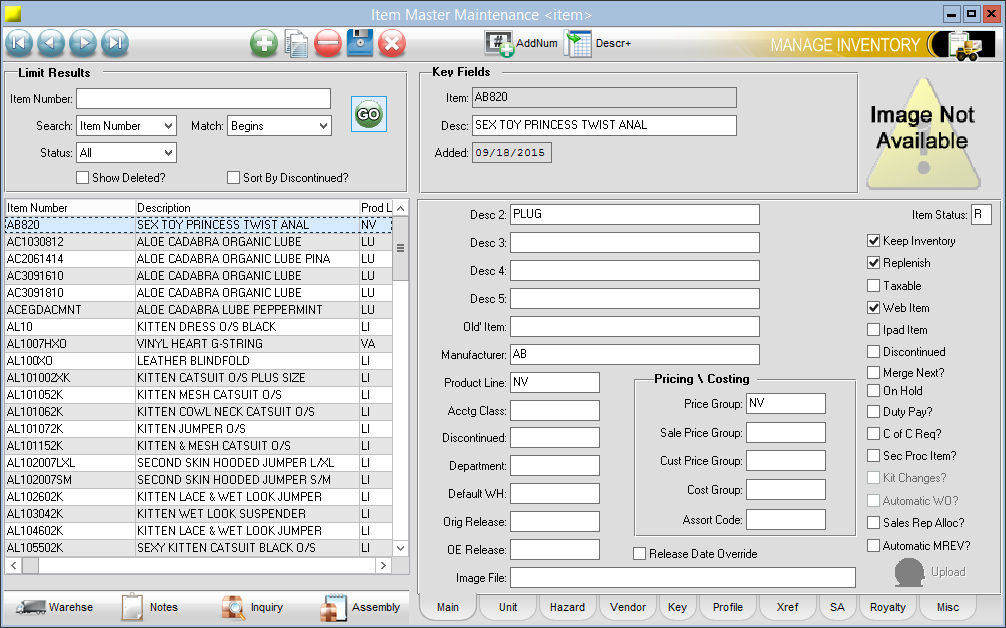
\includegraphics[width=\textwidth]{../img/image55}
		\caption{ITEM Item Master Maintenance Main Tab}
	\end{figure}
	\item Main Tab	
	\begin{itemize}
		\item Item \textemdash Enter item number of click on the add by number and it will give you the next available item number
		\item Desc. \textemdash Enter item description, 1-5 are available for item description, if there is data in the fields it will print on standard forms. Each description field is 30 characters long
		\item Old' Item \textemdash Cross reference field
		\item Product Line \textemdash Required field, pressing F1 in this field will open \texttt{ITPLM} double click on the product line and click enter
		\item Manufacturer \textemdash Open field to put in manufacturer's name or code
		\item Image File \textemdash Link image of product display in upper right hand corner and print on labels; imaghe file must be saved on server to activate and you may use the F1 browser to find the file
		\item Pricing \ Costing
		\begin{itemize}
			\item Pressing F1 in the following 4 fields opens \texttt{ITPG}
			\begin{itemize}
				\item Price Group \textemdash groups items together for pricing
				\item Sale Price Group \textemdash groups items for sale pricing
				\item Cust Price Group \textemdash groups items for special pricing
				\item Cost Group \textemdash groups items for purchase costing
			\end{itemize}
			\item Assort Code \textemdash Pressing F1 in this field opens \texttt{ITACDI} and allows you to set up items for quantity discount pricing
		\end{itemize}
		\item Item Status \textemdash Pressing F1 in this field opens System Help, so you can decide what item status you want. Enter the letter and click enter.
		\begin{itemize}
			\item R \textemdash Regular warehouse item
			\item S \textemdash Special item or for specific customers
			\item D \textemdash Obsolete "Discontinued" (also use checkbox \& date)
			\item A \textemdash Kit/assembly item
			\item N \textemdash Obsolete "Non Stock" or Drop Ship item
		\end{itemize}
		\item Checkboxes
		\begin{itemize}
			\item Keep Inventory \textemdash Keeps quantity count in \texttt{WAITM}
			\item Replenish \textemdash Will show on purchase order reports to buy
			\item Taxable \textemdash Items are usually taxable (Customer setup will determine final sales tax decision)
			\item Web item \textemdash Item is a web item for ecommerce
			\item Discontinued \textemdash Item is discontinued and auto populates current day into the discontinued date field when checked
			\item C of C Req. \textemdash Item includes a certificate of compliance			
		\end{itemize}		
	\end{itemize}
	\begin{figure}[H]
		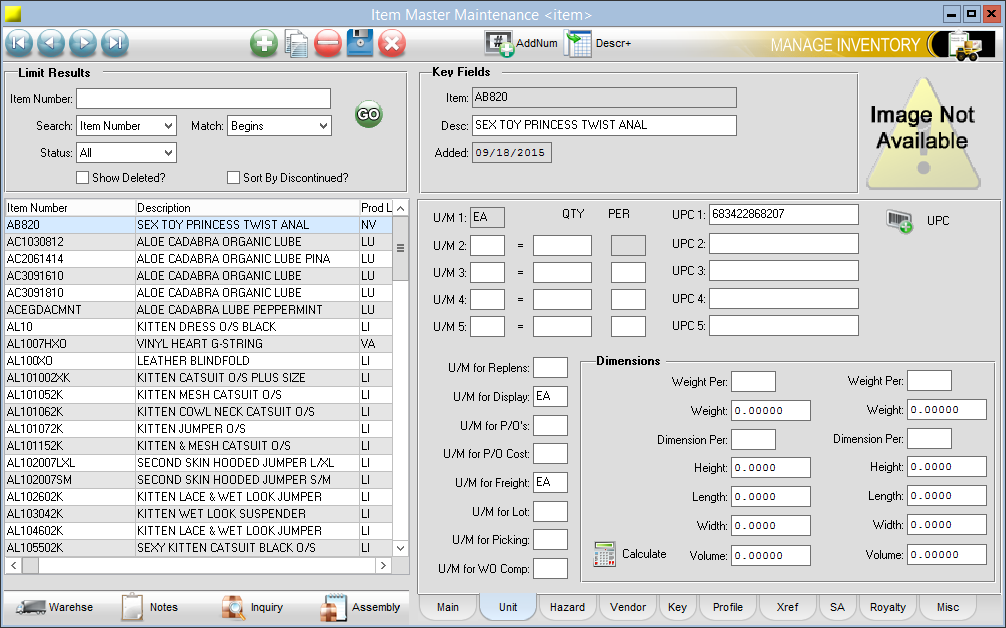
\includegraphics[width=\textwidth]{../img/image56}
		\caption{ITEM Item Master Maintenance Unit Tab}
	\end{figure}
	\item Unit Tab (requires \texttt{ITUMM} setup first)
	\begin{itemize}
		\item Unit of Measures required, start with smallest needed for item
		\begin{itemize}
			\item U/M 1 \textemdash A quantity used as a standard of measurement, starting with the lowest unit of measure \texttt{ITUMI}
			\item U/M 2-5 \textemdash Optional field, option U/M defaults
			\item QTY \textemdash The quantity of lower U/M for the U/M level chosen
			\item PER \textemdash Based on other U/M setup against item
			\item UPC \textemdash Universal Product Code for each U/M, optional
			\item U/M for Replens \textemdash U/M for replenishing inventory
			\item U/M for Display \textemdash U/M that displays in system, this will be the default for all if no other field is filled in
			\item U/M for P/O's \textemdash U/M for purchase orders
			\item U/M for P/O Cost \textemdash U/M for costing
			\item U/M for Freight \textemdash U/M for freight
			\item U/M for Lot \textemdash U/M for lots
			\item U/M for Picking \textemdash U/M for picking product
			\item U/M for WO Comp \textemdash U/M to use as Work Order Components
		\end{itemize}
		\item Dimensions / Weight Per \textemdash For shipping purposes
		\begin{itemize}
			\item Weight per \textemdash U/M
			\item Weight \textemdash Weight
		\end{itemize}
	\end{itemize}
	\begin{figure}[H]
		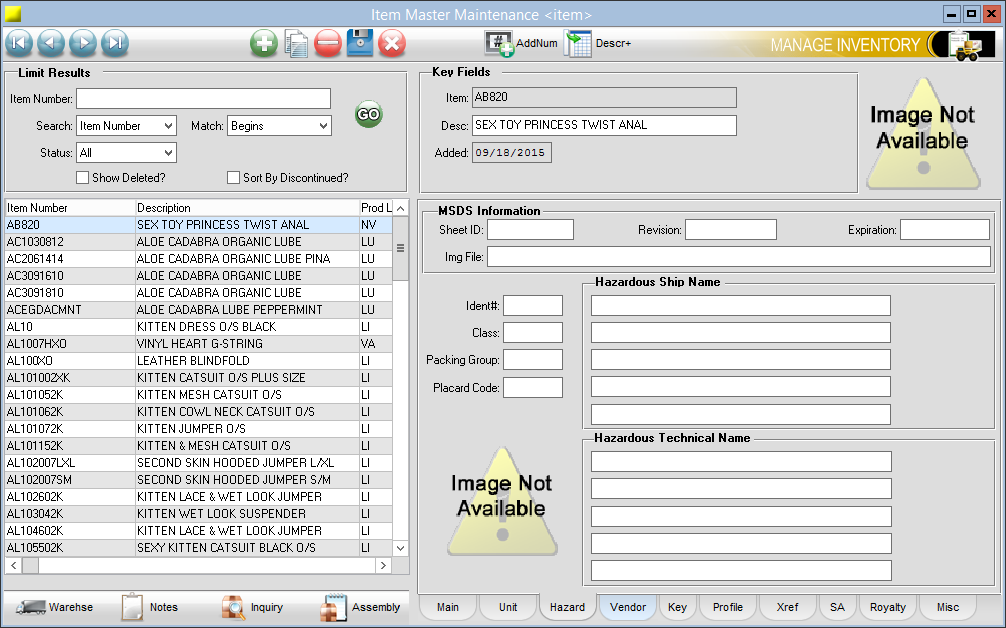
\includegraphics[width=\textwidth]{../img/image57}
		\caption{ITEM Item Master Maintenance Hazard Tab}
	\end{figure}
	\item Hazard Tab \\
	If item has hazardous material and requires an MSDS sheet, store data and link MSDS sheet. Image needs to be stored on server first.
	\begin{figure}[H]
		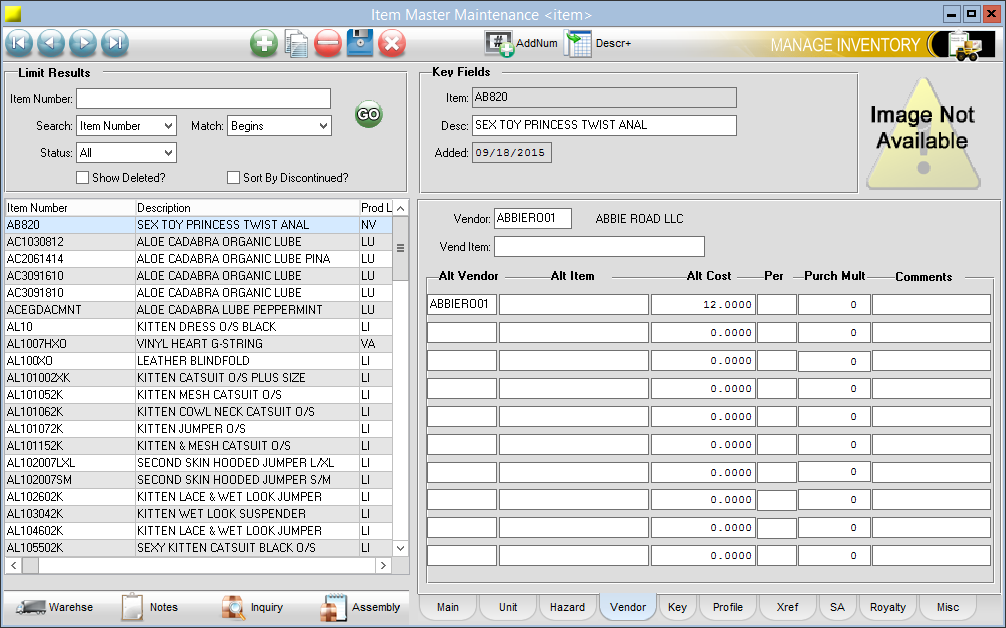
\includegraphics[width=\textwidth]{../img/image58}
		\caption{ITEM Item Master Maintenance Vendor Tab}
	\end{figure}
	\item Vendor Tab \textemdash To select primary vendor for this item
	\begin{itemize}
		\item Vendor \textemdash Enter primary vendor or use F1 to open \texttt{VEMM}
		\begin{itemize}
			\item Vend Item \textemdash Enter rpimary vendor part number, this is also a cross reference
		\end{itemize}
		\item Alt Vendor \textemdash Store alternative vendor for item, using F1 in this field opens \texttt{VEMM}
		\begin{itemize}
			\item Alt Item \textemdash Enter alternative item number
			\item Alt Cost \textemdash Enter alternative cost
			\item Purch Mult. \textemdash Quantity amount that vendor requires to purchase
		\end{itemize}
	\end{itemize}
	\begin{figure}[H]
		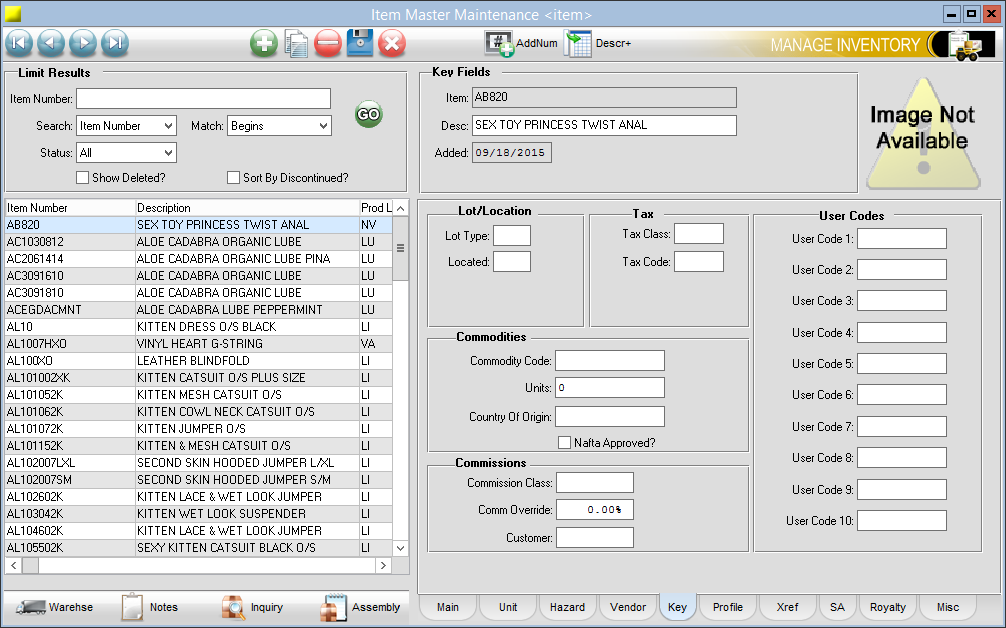
\includegraphics[width=\textwidth]{../img/image59}
		\caption{ITEM Item Master Maintenance Key Tab}
	\end{figure}
	\item Key Tab
	\begin{itemize}
		\item Lot / Location (see \texttt{XO} System Option called "lot\_loc\_setup" for selected table to keep lot and location information in V2)
		\begin{itemize}
			\item Lot Type \textemdash Identifier for an item as being serialized or lot controlled. This would be applied to all warehouses
			\item F1 opens System Help for types of lots
			\begin{itemize}
				\item F \textemdash First In, First Out
				\item L \textemdash Last In, Last Out
				\item MF \textemdash Manual In, First Out
				\item M \textemdash Always manually assign lots
				\item SS \textemdash Must assign lot / serial number when shipping for each quantity; no lot assignment when receiving
				\item SM \textemdash Must always assign lot / serial number manually for each quantity
				\item SA \textemdash Serial lot auto assignment
			\end{itemize}
			\item Located \textemdash Identify where the lot items are located
			\begin{itemize}
				\item Blank \textemdash Not Located
				\item A \textemdash Always use default receiving / shipping locations
				\item D \textemdash Use default receiving location; ship from locations with available quantity then default shipping location
				\item M \textemdash Always manually assign location
				\item L \textemdash Located item with lots; use lot setup
			\end{itemize}
		\end{itemize}
	\end{itemize}
	\begin{figure}[H]
		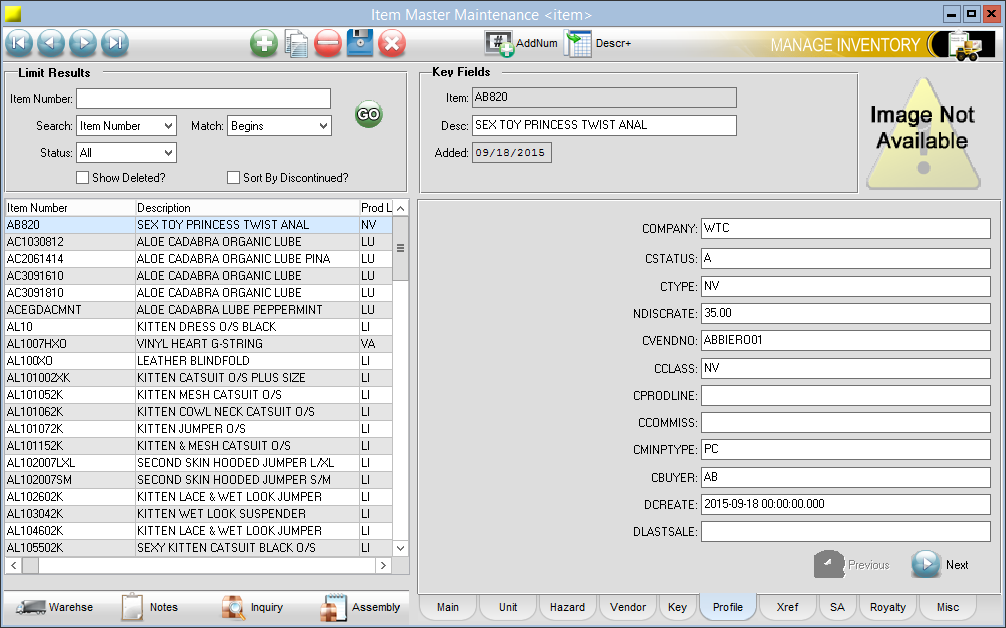
\includegraphics[width=\textwidth]{../img/image60}
		\caption{ITEM Item Master Maintenance Profile Tab}
	\end{figure}
	\item Profile Tab\\
	60 additional fields to rename and use as you want. Able to print on forms and reports.
	\begin{figure}[H]
		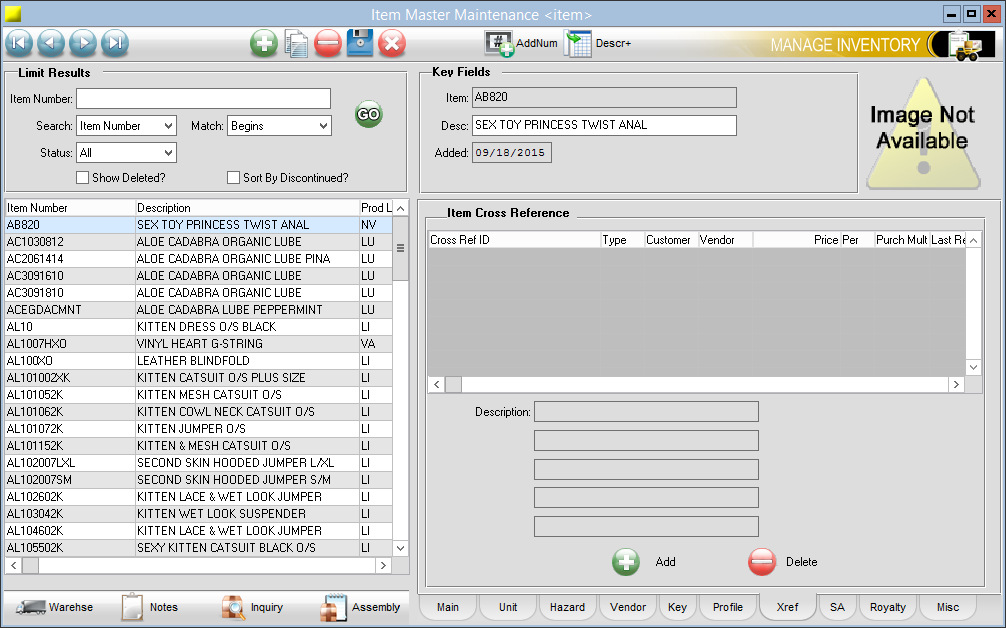
\includegraphics[width=\textwidth]{../img/image61}
		\caption{ITEM Item Master Maintenance Xref Tab}
	\end{figure}
	\item Xref Tab \textemdash To identify the item by using a different name or number that is not your main part number
	\begin{itemize}
		\item Cross Ref ID \textemdash Enter cross reference ID
		\item Type \textemdash Enter a number or code to identify type (optional), setup in \texttt{ITXFRTM}
		\item Customer \textemdash Account Number (optional)
		\item Vendor \textemdash Vendor Number (optional)
		\item Price \textemdash Fixed sell price (optional)
	\end{itemize}
\end{enumerate}

\subsubsection{Warehouse Item Maintenance}

\index{ERP-One Commands!WAITM}

The \texttt{WAITM} command is used to access Warehouse Item Maintenance

\begin{enumerate}
	
	\begin{figure}[H]
		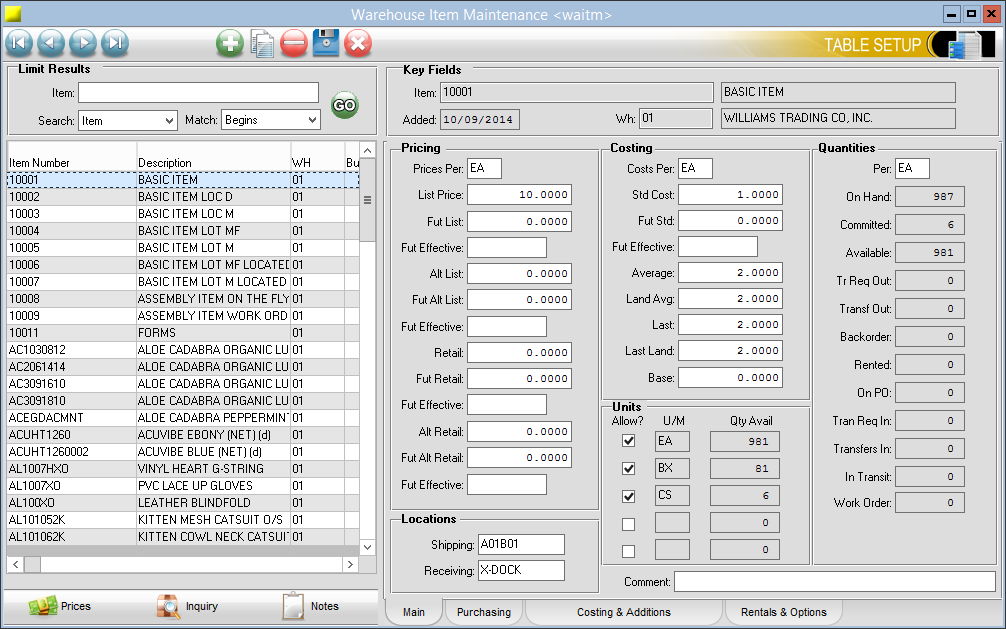
\includegraphics[width=\textwidth]{../img/image62}
		\caption{WAITM Warehouse Item Maintenance Main Tab}
	\end{figure}
	
	\item Main Tab
	\begin{itemize}
		\item Pricing \textemdash all options excluding Price Per are optional
		\begin{itemize}
			\item Price per \textemdash Enter E/M for List Price (required field)
			\item List Price \textemdash Enter list price
			\item Fut List \textemdash Enter a future list price
			\item Fut Effective \textemdash Date of future list to activate
			\item Alt List \textemdash Enter an alternate price
			\item Retail \textemdash Retail price
			\item Fut Retail \textemdash Future retail price
			\item Fut Effective \textemdash Date of future price to activate
			\item Alt Retail \textemdash Alternate retail price
		\end{itemize}
		\item Costing \textemdash used for PO's and costing for sales orders
		\begin{itemize}
			\item Manually Maintained
			\begin{itemize}
				\item Cost Per \textemdash U/M for cost price (required field)
				\item Std Cost \textemdash Standard Cost
				\item Fut Std \textemdash Future Standard Cost
				\item Fut Effective \textemdash Date of future standard cost to activate
				\item Base \textemdash Base Cost				
			\end{itemize}
			\item Auto Adjusted
			\begin{itemize}
				\item Average \textemdash Average Cost
				\item Land Avg. \textemdash Landed Average Cost
				\item Last \textemdash Last Cost
				\item Last Land \textemdash Last Landed Cost
			\end{itemize}
		\end{itemize}
		\item Quantities
		\begin{itemize}
			\item Per \textemdash U/M that On Hand and Committed Quantities are based on
			\item On Hand \textemdash Quantity of the item in the system
			\item Committed \textemdash Quantity committed to order but not processed yet
			\item Available \textemdash Quantity that are not committed to an order
			\item Backorder \textemdash How many are on back order
			\item On PO \textemdash How many are on a purchase order
		\end{itemize}
		\item Allow
		\begin{itemize}
			\item U/M \textemdash Determines what U/M is allowed for item
			\item Qty. Available \textemdash How many are available for the U/M
		\end{itemize}
		\item Locations \textemdash Generic or default locations for warehouse item
		\begin{itemize}
			\item Shipping \textemdash Location to ship from
			\item Receiving \textemdash Location for receiving
		\end{itemize}
	\end{itemize}
		
	\begin{figure}[H]
		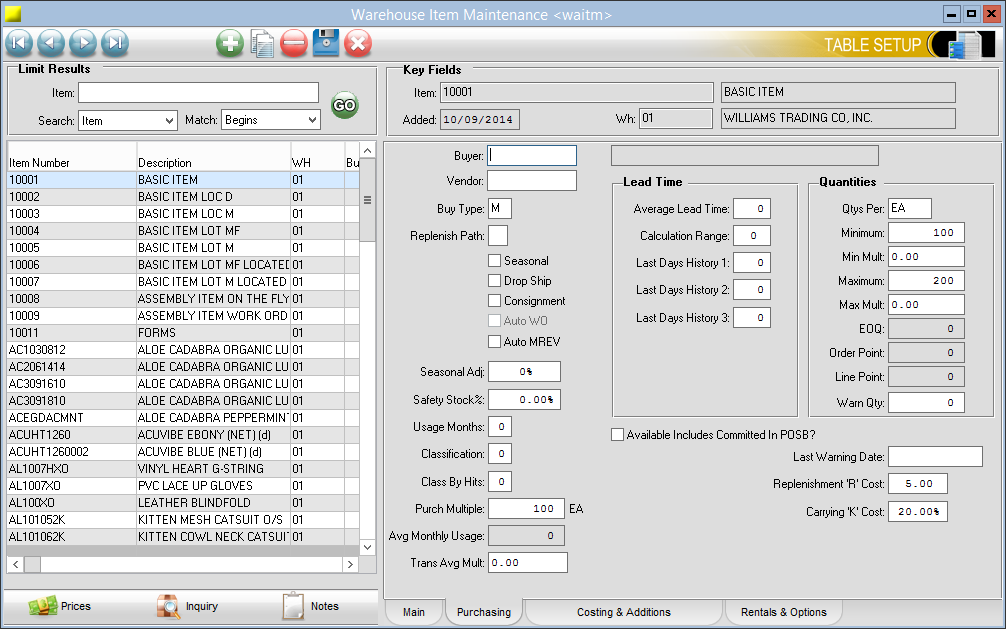
\includegraphics[width=\textwidth]{../img/image63}
		\caption{WAITM Warehouse Item Maintenance Purchasing Tab}
	\end{figure}
		
	\item Purchasing Tab
	\begin{itemize}
		\item Buy Type \textemdash The 'Suggested Buy' type indicates the method used to calculate a suggested quantity to reorder for a warehouse item.
		\begin{itemize}
			\item E \textemdash Economic Order Quantity method
			\item C \textemdash Item Usage Classification method
			\item M \textemdash Minimum / Maximum calculation method
			\item H \textemdash Hits default setting to determine replenishment
		\end{itemize}
		\item Purch Multiple \textemdash Increments for purchasing
		\item Lead Time\\
		Average lead Time \textemdash Calculated average time to receive item into stock after ordering (see \texttt{ITRPU} and \texttt{ITRPM} instructions)		
		\item Quantities \textemdash Settings for Buy Type
		\begin{itemize}
			\item Qtys. Per \textemdash U/M for stock
			\item M \textemdash Minimum / Maximum calculation method drives:
			\begin{itemize}
				\item Minimum \textemdash Minimum to keep in stock
				\item Maximum \textemdash Maximum to keep in stock
			\end{itemize}
			\item E \textemdash Economic Order Quantity method drives:
			\begin{itemize}
				\item EOQ
				\item Order Point
				\item Line Point
			\end{itemize}
			\item Warn Qty. \textemdash Optional, when item falls below this quantity, will receive a pop-up warning in Order Entry. \texttt{XO} option named "wa\_disp\_qty\_warn\_msg" must be set to "Yes" to activate
		\end{itemize}
	\end{itemize}
	
	\begin{figure}[H]
		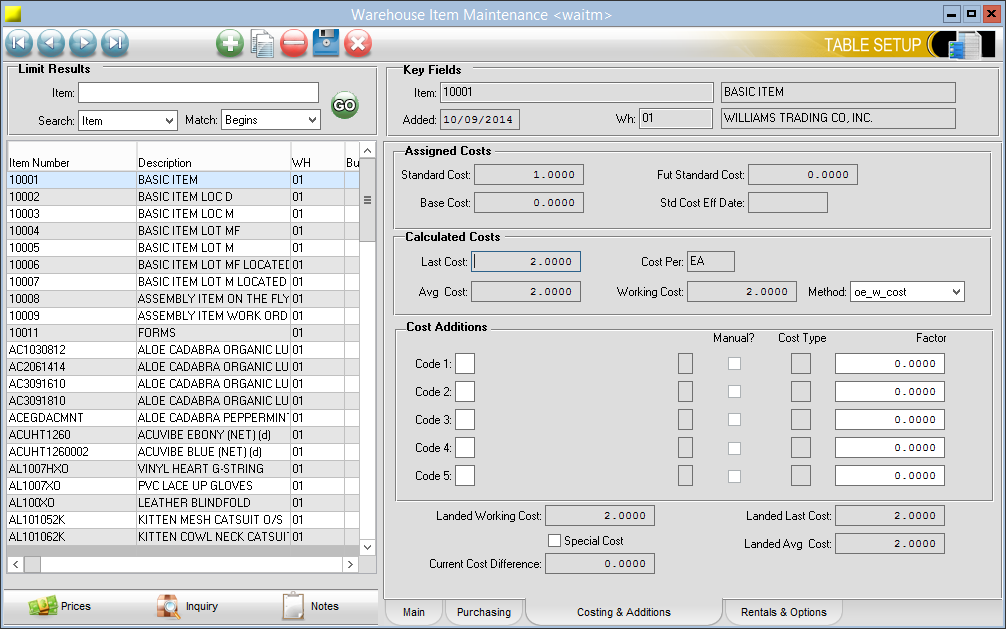
\includegraphics[width=\textwidth]{../img/image64}
		\caption{WAITM Warehouse Item Maintenance Costing \& Additions Tab}
	\end{figure}
	
	\item Costing and Additions Tab\\
	Setup in \texttt{POACM} affects landed costs
	\begin{itemize}
		\item Cost Additions \textemdash Codes 1-5 \textemdash Default add on's for item per warehouse
	\end{itemize}
	
	\begin{figure}[H]
		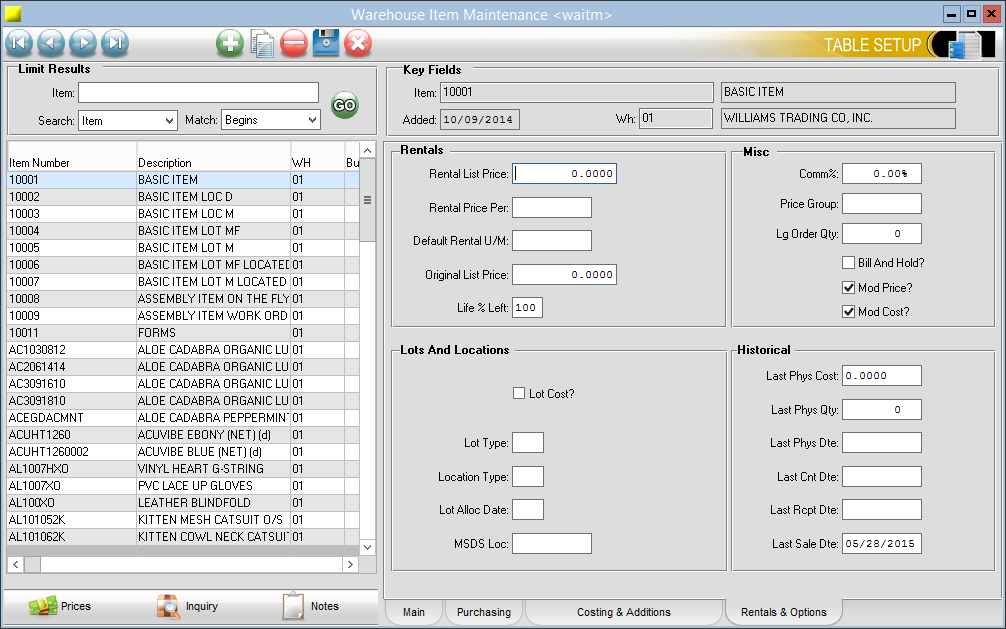
\includegraphics[width=\textwidth]{../img/image65}
		\caption{WAITM Warehouse Item Maintenance Rentals and Options Tab}
	\end{figure}
	
	\item Rentals and Options Tab
	\begin{itemize}
		\item If lot and located table is set to WA\_ITEM in \texttt{XO} called "lot\_loc\_setup", use the fields on this tab to indicate lot and / or location type and lot cost.
		\item Set the rental information if the item in this warehouse is rented out to customers
	\end{itemize}
\end{enumerate}

\subsubsection{Item Notes Maintenance}

\index{ERP-One Commands!ITNM}

The \texttt{ITNM} command is used to access Item Notes Maintenance

\begin{figure}[H]
	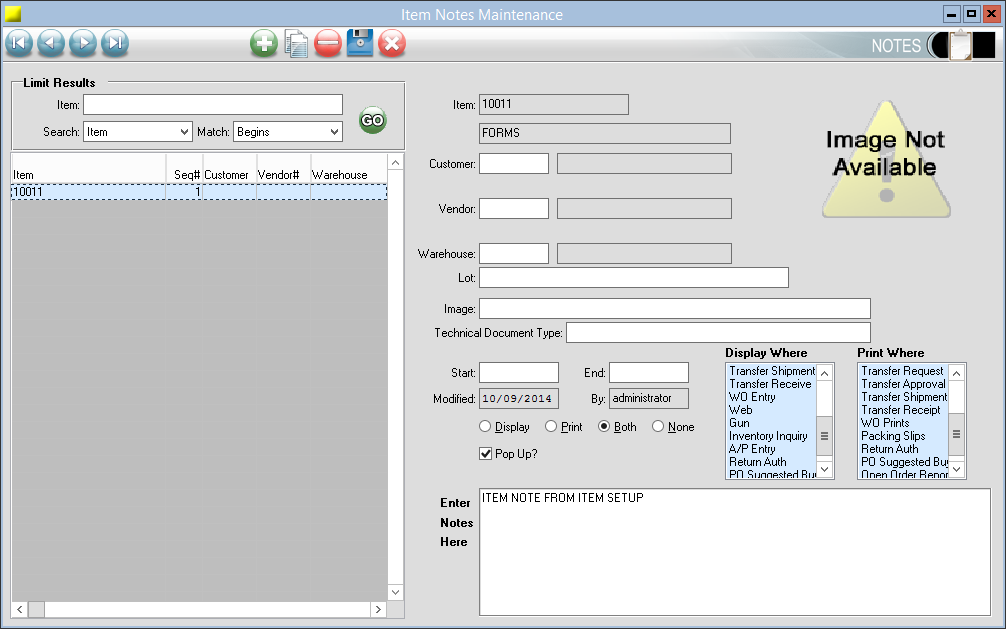
\includegraphics[width=\textwidth]{../img/image66}
	\caption{ITNM Item Notes Maintenance}
\end{figure}

You can set a note at item level. Notes can also be entered in at time of order entry or purchase order entry, per order or line item. Within notes, you have options on where, when, and what you would like it to print on. You can choose for it to be a pop up and / or display. You may also have an expiration date of when you no longer want the note to be active.

\subsection{Vendor Maintenance}

\subsubsection{Vendor Master Maintenance}

\index{ERP-One Commands!VEMM}

The \texttt{VEMM} command is used to access Vendor Master Maintenance

\begin{enumerate}
	
	\begin{figure}[H]
		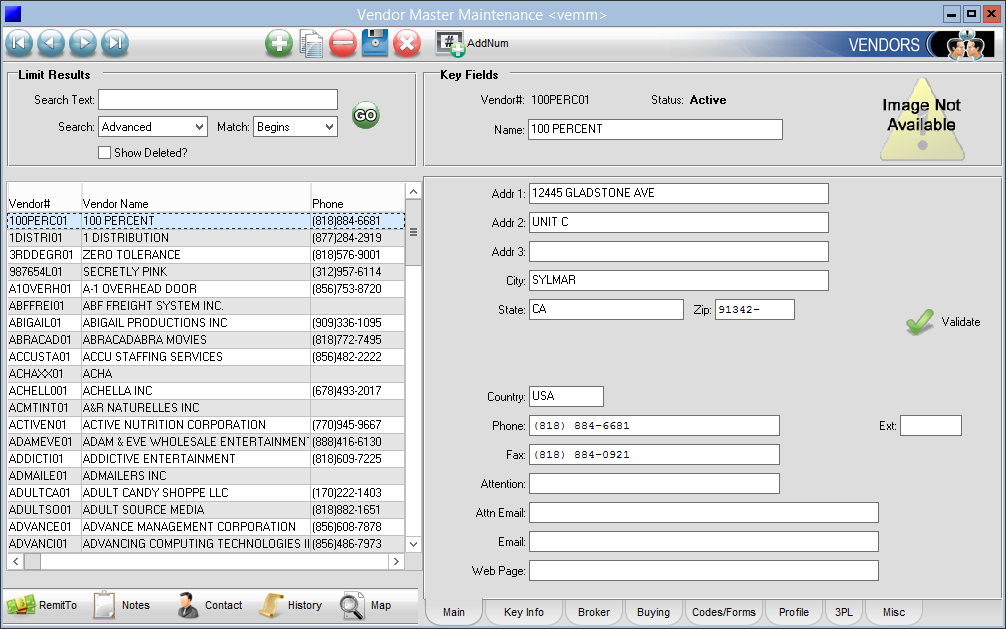
\includegraphics[width=\textwidth]{../img/image67}
		\caption{VEMM Vendor Master Maintenance Main Tab}
	\end{figure}
	
	\item Main Tab \textemdash This is where the core data for the vendor is stored. It will default into the puchase order entry screen and may be overridden as the PO is created
	\begin{itemize}
		\item Vendor Account Number Field \textemdash In this field you will add a unique vendor ID (numbers and letters allowed.) The ID can not be duplicated.
		\item Name \textemdash Enter vendor name
		\item Country \textemdash Based upon country codes, dictates how the address screen is laid out. Using F1 in this field opens a list of country codes.
		\item Address \textemdash Address 1 is the main address
		\item Attention \textemdash Primary contact
		\item Attention Email \textemdash Primary email address
		\item Email \textemdash Primary email for vendor
		\item Webpage \textemdash Vendor's web page		
	\end{itemize}	
	
	\begin{figure}[H]
		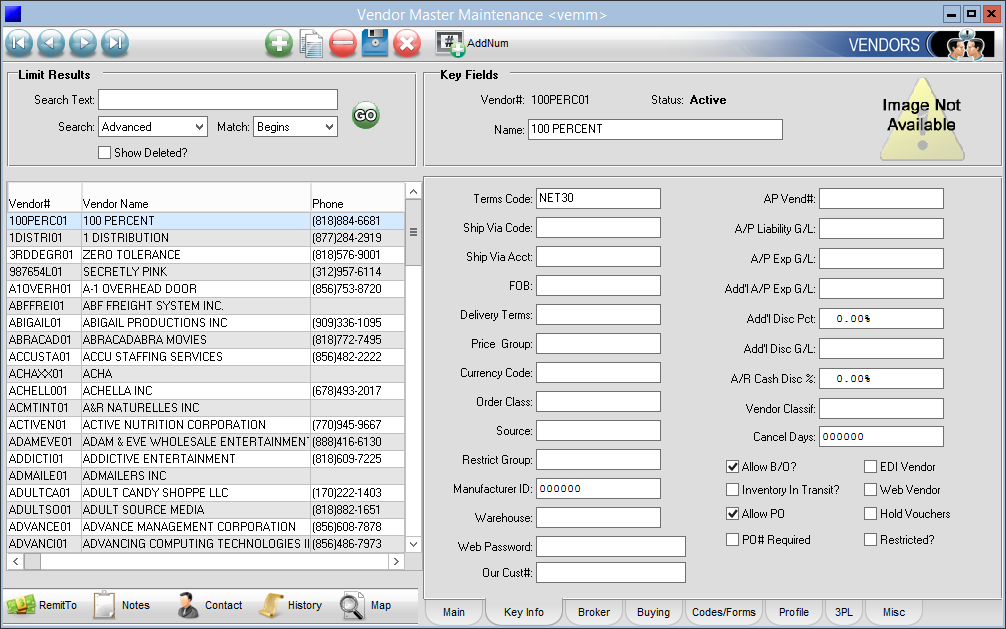
\includegraphics[width=\textwidth]{../img/image68}
		\caption{VEMM Vendor Master Maintenance Key Info Tab}
	\end{figure}
	
	\item Key Info Tab
	\begin{itemize}
		\item Terms Code \textemdash Terms with vendor, using F1 will bring up \texttt{SYTCM}
		\item Ship Via Code \textemdash Default how you want product shipped to you, can be overridden at purchase order entry. Using F1 in this field will bring up \texttt{SYSVM}. May print on purchase order.
		\item Ship Via Acct \textemdash Your account number with shipping company for collect, prints on purchase order.
		\item Currency Code \textemdash Using F1 in this field will bring up currency options \texttt{SYCRM}
		\item Web Password \textemdash Store password for vendor website
		\item Our Customer \# \textemdash Your customer number with the vendor
		\item A/P Liability G/L \textemdash Optional override of default A/P account
		\item A/P Exp G/L \textemdash Inventory GL / Utility GL for vendor
		\item Add'l A/P Exp. G/L \textemdash Typically freight in GL (These are default GL for AP Vouchers)
	\end{itemize}
	
	\begin{figure}[H]
		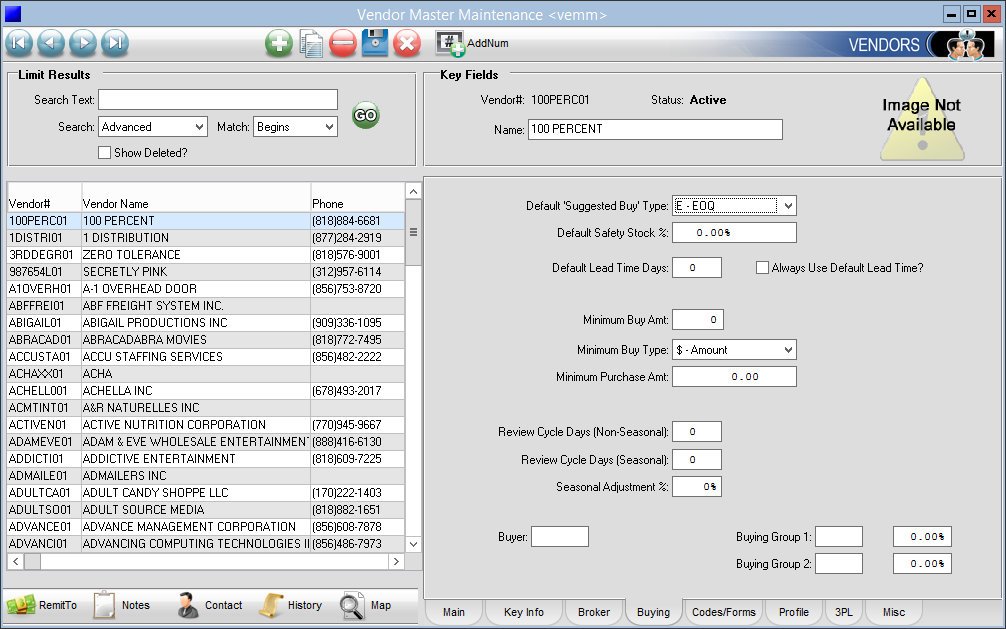
\includegraphics[width=\textwidth]{../img/image69}
		\caption{VEMM Vendor Master Maintenance Buying Tab}
	\end{figure}
	
	\item Buying Tab \textemdash Default setting for purchasing
	\begin{itemize}
		\item Minimum Buy Amount \textemdash How much in amount or weight, based on buy type
		\item Minimum Buy Type \textemdash Purchase requirements, in amount or weight, based on buy type, the above MIN/MAX work together
		\item Minimum Purchase Amount \textemdash If vendor requires the purchase to reach a minimum buy amount. If you don't meet the criteria upon accepting the purchase order, you will get a pop up warning, but the order can still be placed
	\end{itemize}
	
	\begin{figure}[H]
		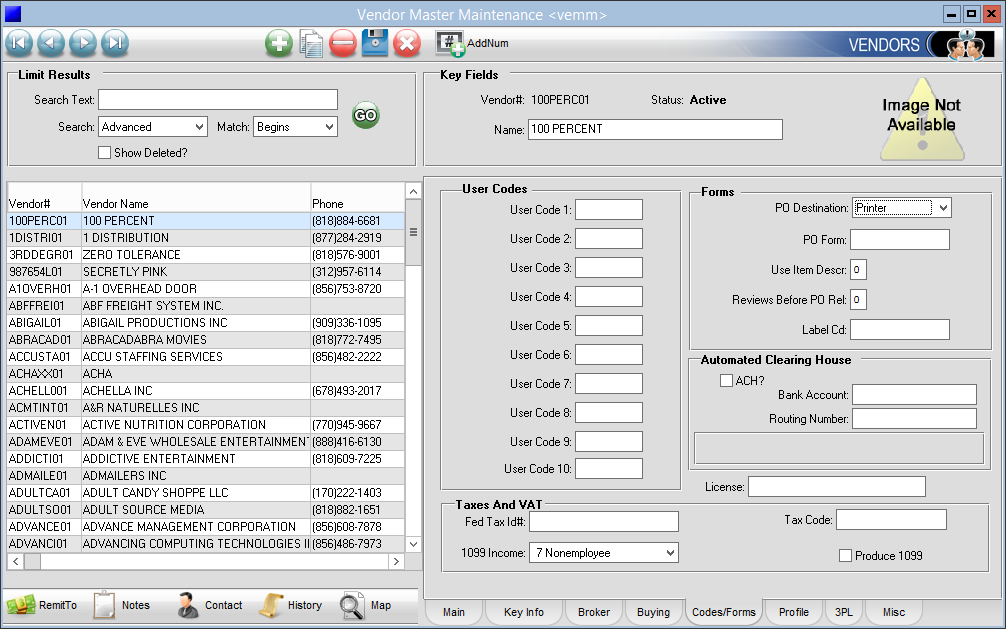
\includegraphics[width=\textwidth]{../img/image70}
		\caption{VEMM Vendor Master Codes / Forms Tab}
	\end{figure}
	
	\item Codes / Forms Tab
	\begin{itemize}
		\item User Codes \textemdash Ten user codes to use any way you want for reporting purposes. Option to print on documents.
		\item Forms
		\begin{itemize}
			\item PO Destination \textemdash Default setting for how you want the purchase order to print, email or fax.			
		\end{itemize}
		\item Taxes and VAT
		\begin{itemize}
			\item If 1099 type vendor, check the option to produce 1099
		\end{itemize}
	\end{itemize}
	
	\begin{figure}[H]
		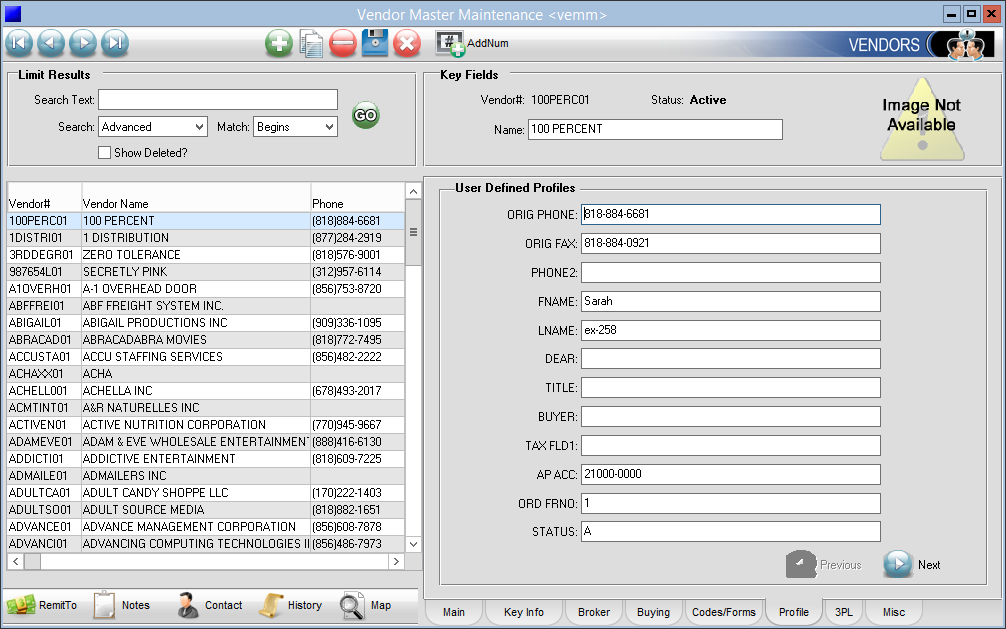
\includegraphics[width=\textwidth]{../img/image71}
		\caption{VEMM Vendor Master Profile Tab}
	\end{figure}
	
	\item Profile Tab
	\begin{itemize}
		\item Profile Info \textemdash Sixty additional fields you can label in \texttt{SYPROF} and create F1 lookup tables in \texttt{VEPF1}
	\end{itemize}
\end{enumerate}

\subsubsection{Vendor Remit To Maintenance}

\index{ERP-One Commands!VEREM}

The \texttt{VEREM} command is used to access Vendor Remit To Maintenance.

\begin{figure}[H]
	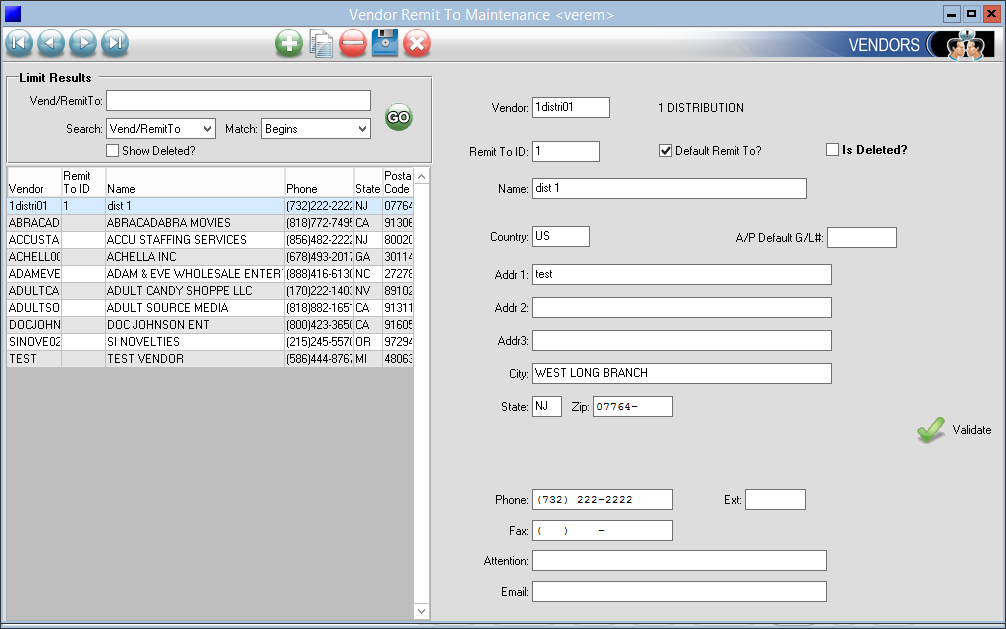
\includegraphics[width=\textwidth]{../img/image72}
	\caption{VEREM Vendor Remit To Maintenance}
\end{figure}

\begin{itemize}
	\item To add a new remit to, click on the add button. This opens up the Remit to ID.
	\item Remit to ID \textemdash In this field you will add a unique ID (numbers and letters allowed.) The ID can not be duplicated.
	\item Name \textemdash Enter Remit To name
	\item Country \textemdash Required field. Country code determines how the address screen is paied out. Use F1 to find country code.
	\item Address \textemdash Address 1 is the Remit To address for payments
	\item Phone / Fax \textemdash Remit To phone and fax
	\item Attention \textemdash Remit To contact
	\item Email \textemdash Remit To Email Address
	\item Webpage \textemdash Vendor's web page
	\item After you have completed your data entry, click save
\end{itemize}

\subsubsection{Vendor Master Maintenance Notes}

\index{ERP-One Commands!VENM}

The \texttt{VENM} command is used to access Vendor Notes Maintenance.

\begin{figure}[H]
	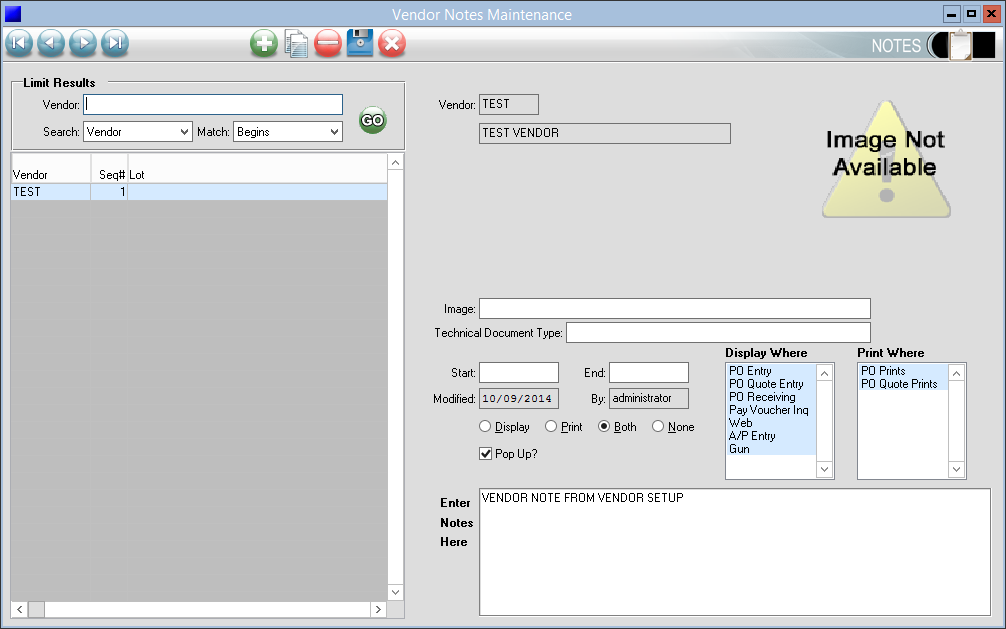
\includegraphics[width=\textwidth]{../img/image73}
	\caption{VENM Vendor Master Maintenance Notes}
\end{figure}

You can create a note at the vendor level. Notes can also be entered in at time of purchase order entry, per order or line item. Within notes, you have options as to where the note will display in ERP One and on what forms you would like it to print. You can choose for it to be a pop up and / or display. You may also have an expiration date for when you no longer want that note to be active.

\subsubsection{Vendor Contacts Maintenance}

\index{ERP-One Commands!VECOM}

The \texttt{VECOM} command is used to access Vendor Contacts Maintenance.

\begin{figure}[H]
	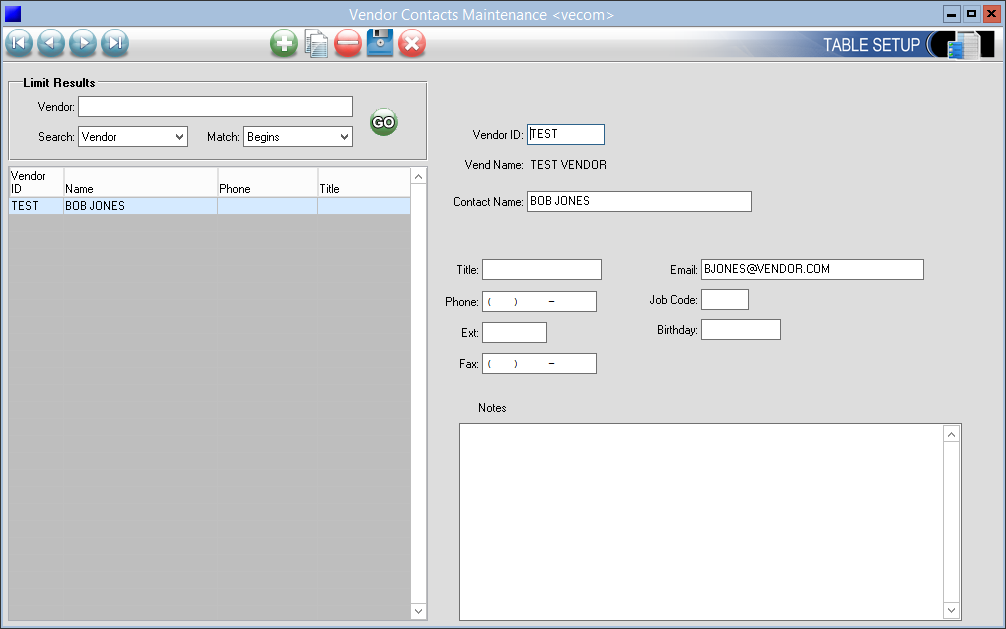
\includegraphics[width=\textwidth]{../img/image74}
	\caption{VENM Vendor Master Maintenance Notes}
\end{figure}

Vendor contacts can be added during vendor set up and can be added during purchase order entry. To add in purchase order entry, while in the header screen, hover over the Vendor Contact on the left. A clickable button appears, which you can click on and enter contact information then click Save. The next time you are placing an order you can use F1 in that field and bring up the saved contacts.

\subsection{Customer Maintenance}

\subsubsection{Customer Master Maintenance}

\index{ERP-One Commands!CUMM}

The \texttt{CUMM} command is used to access Customer Master Maintenance.

\begin{enumerate}
	
	\begin{figure}[H]
		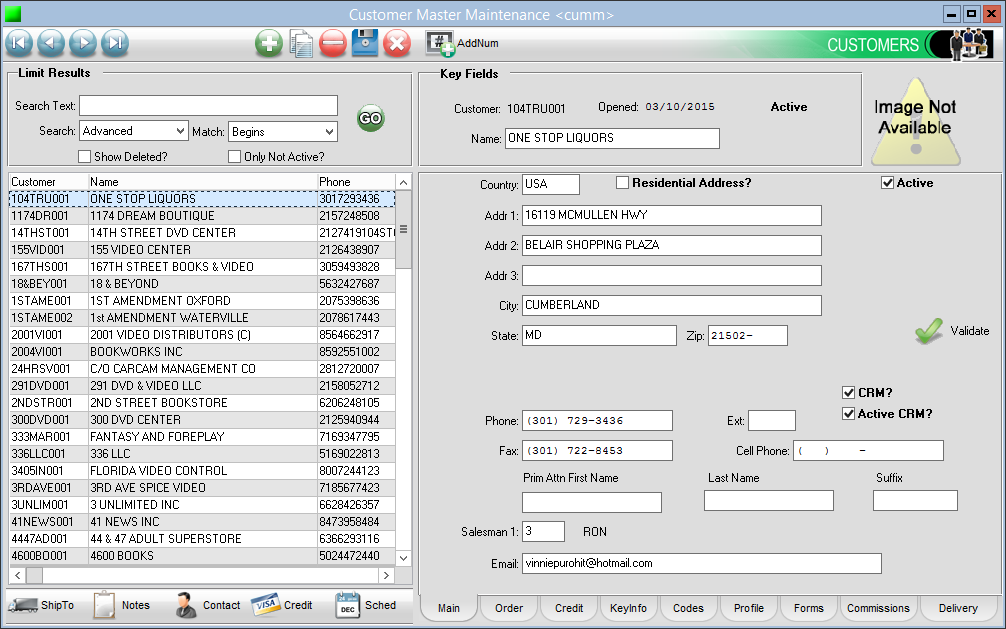
\includegraphics[width=\textwidth]{../img/image75}
		\caption{CUMM Customer Master Maintenance Main Tab}
	\end{figure}
	
	\item Main Tab \textemdash This is where all the core data for the customer is stored. The data that is stored for the customer will default into the order entry screen when placing an order. Default data can be overridden in order entry.
	\begin{itemize}
		\item Customer Field \textemdash In this field you will add a unique customer ID, (nummbers and letters allowed.) The ID can not be duplicated.
		\item Name \textemdash Enter customer name
		\item Country \textemdash Based upon Country Code, dictates how the address screen is laid out. Using F1 in this field opens a list of countries. Choose country by double clicking and then clicking Enter.
		\item Address \textemdash Address 1 is the true address.
		\item Map \textemdash Linked to Yahoo! maps.
		\item Active \textemdash If checked, customer is active
		\item Phone / Fax \textemdash Enter main number for customer
		\item Prime Attn. \textemdash Enter primary contact for customer
		\item Salesman 1 \textemdash Required field. Using F1 in this field opens up a list of sales people.
		\item Email \textemdash Enter primary email contact
	\end{itemize}
	
	\begin{figure}[H]
		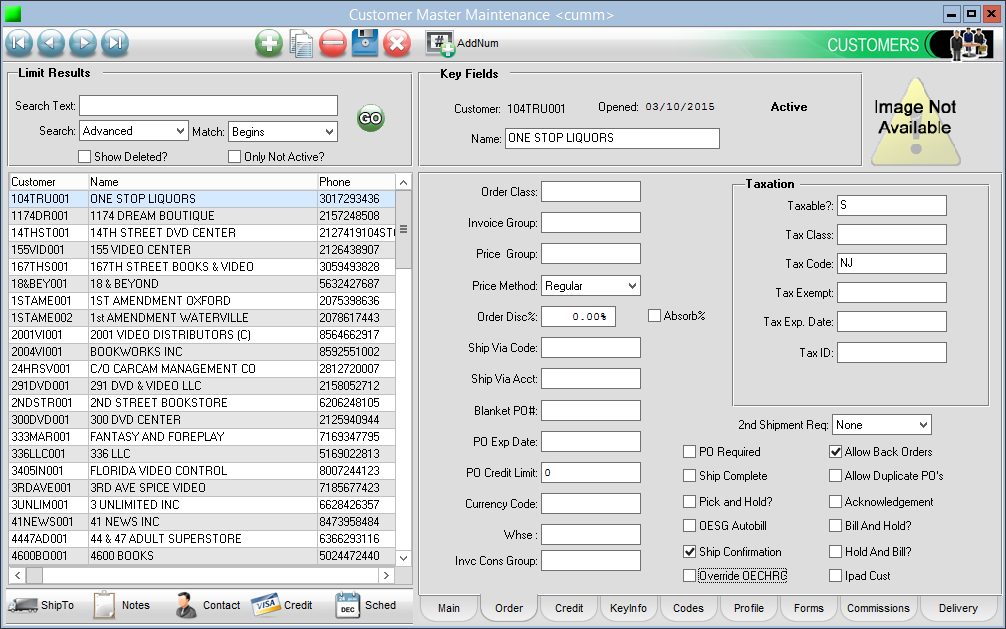
\includegraphics[width=\textwidth]{../img/image76}
		\caption{CUMM Customer Master Maintenance Order Tab}
	\end{figure}
	
	\item Order Tab \textemdash Set certain criteria of how the customer wants their orders handled.
	\begin{itemize}
		\item Ship Via Code \textemdash The way the order ships from the warehouse to the customer. Use F1 to access \texttt{SYSVM} for the options of shipping codes
		\item Ship Via Acct \textemdash Enter customer shipping account if required
		\item Taxation (Per Order or Line Item)
		\begin{itemize}
			\item Taxable \textemdash Required field. This is how the customer will be taxed. Using F1 will display the following options:
			\begin{itemize}
				\item Always \textemdash Customer is always taxed
				\item Never \textemdash Customer is never taxed (Tax Code required)
				\item Sometimes \textemdash Whether order is taxed is prompted for at order entry
			\end{itemize}
			\item Tax Code \textemdash Required field. Set up percentages of the tax according to state, country, jurisdictions etc.. Using F1 in this field will open \texttt{CUTXM}
			\item Tax Exempt \textemdash If customer is tax exempt, you can store the tax exempt number in this field
			\item Tax Exempt Date \textemdash Tax exempt number expiration date is displayed in order entry
		\end{itemize}
		\item Checked
		\begin{itemize}
			\item PO Required \textemdash Require a PO before you are able to leave the header screen in Order Entry
			\item Ship Complete \textemdash ERP One allocates the items in stock, will not print or prompt to print pick ticket until the order is 100% complete
			\item Pick and Hold \textemdash ERP One allocates the items, will print pick ticket and items will be put in a staging area until order is completed
			\item $2^{nd}$ Shipment Req \textemdash you have options also for a second shipment, to ship complete or pick and hold
			\item Allow Back Orders \textemdash If checked, allows back orders, unchecked will consider the order complete and not backorder items
			\item Allow Duplicate PO's \textemdash If checked will PO numbers to be used more than once
			\item Acknowledgment \textemdash If checked, allows an acknowledgment to print for the customer
		\end{itemize}
	\end{itemize}
	
	\begin{figure}[H]
		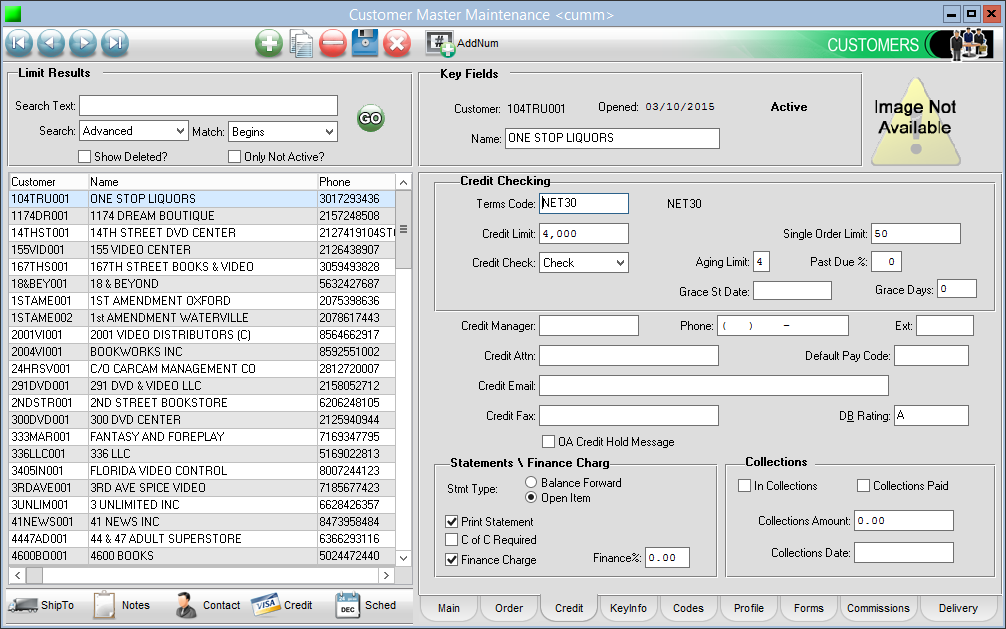
\includegraphics[width=\textwidth]{../img/image77}
		\caption{CUMM Customer Master Maintenance Credit Tab}
	\end{figure}
	
	\item Credit Tab
	\begin{itemize}
		\item Terms Code \textemdash Payment terms with customer, drives invoice aging and discount on AR side for cash receipts. Using F1 in this field will bring up \texttt{SYTCM}
		\item Credit Limit \textemdash Dollar amount for credit limit if credit is checked
		\item Credit Check
		\begin{itemize}
			\item Always Pass \textemdash Always pass order through, no credit check is done
			\item Check \textemdash Check for status of credit, verify dollar amount and aging
			\item Always Fail \textemdash Always put sales order on credit hold until released
		\end{itemize}
		\item Aging Limit (set by \texttt{XO} options)
		\begin{itemize}
			\item 1 \textemdash 30 days
			\item 2 \textemdash 60 days
			\item 3 \textemdash 90 days
			\item 4 \textemdash 120 days
			\item 5 \textemdash 150 days
		\end{itemize}
		\item Statement \ Finance Charge
		\begin{itemize}
			\item Print Statement \textemdash If checked, will allow an A/R statement to print for the customer
			\item C of C \textemdash If checked, option to print certification of compliance
		\end{itemize}
	\end{itemize}
	
	\begin{figure}[H]
		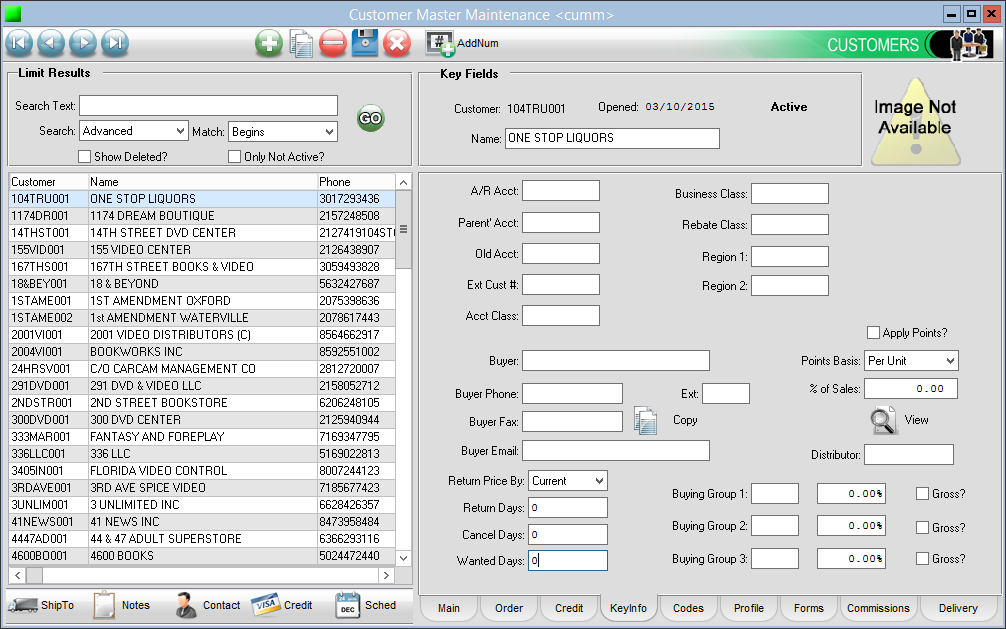
\includegraphics[width=\textwidth]{../img/image78}
		\caption{CUMM Customer Master Maintenance Key Info Tab}
	\end{figure}
	
	\item Key Info Tab
	\begin{itemize}
		\item A/R Acct \textemdash If multiple accounts are in ERP One, but need only one Bill To for cash receipts
		\item Parent' Acct \textemdash If the sales of one account should be reported in another
		\item Business Class \textemdash Selects reporting options, see \texttt{CUBC}
	\end{itemize}
	
	\begin{figure}[H]
		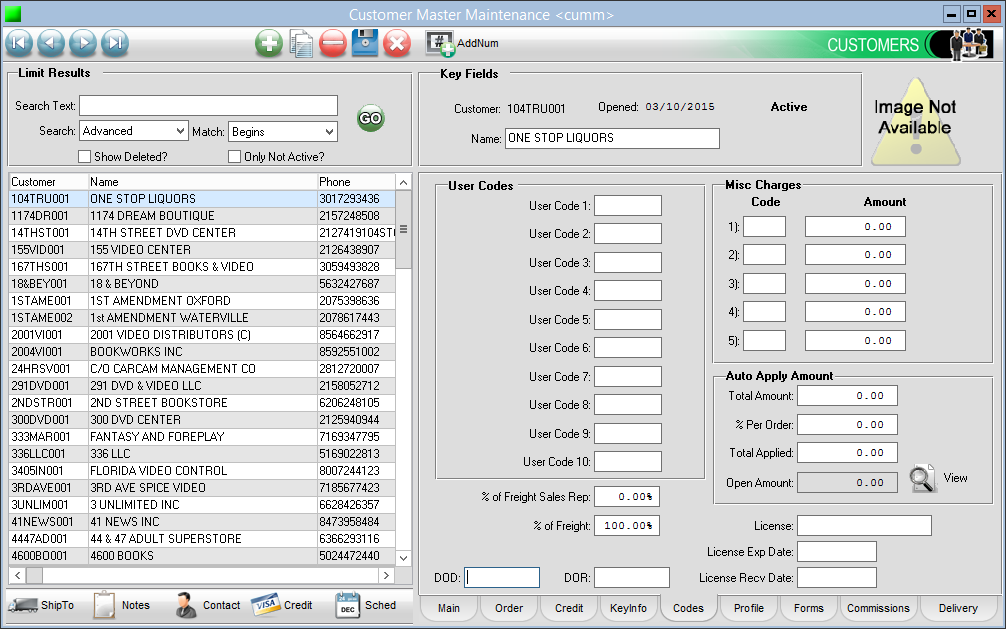
\includegraphics[width=\textwidth]{../img/image79}
		\caption{CUMM Customer Master Maintenance Codes Tab}
	\end{figure}
	
	\item Codes Tab
	\begin{itemize}
		\item User Codes \textemdash Ten user codes to use any way you want for reporting purposes. Option to print on documents.
		\item Misc. Charges
		\begin{itemize}
			\item Code \textemdash Establishes code for additional fee to always apply to customer's orders. Using F1 in this field will open up \texttt{OETCM}.
			\item Amount \textemdash Enter in the amount of additional fee
		\end{itemize}
	\end{itemize}
	
	\begin{figure}[H]
		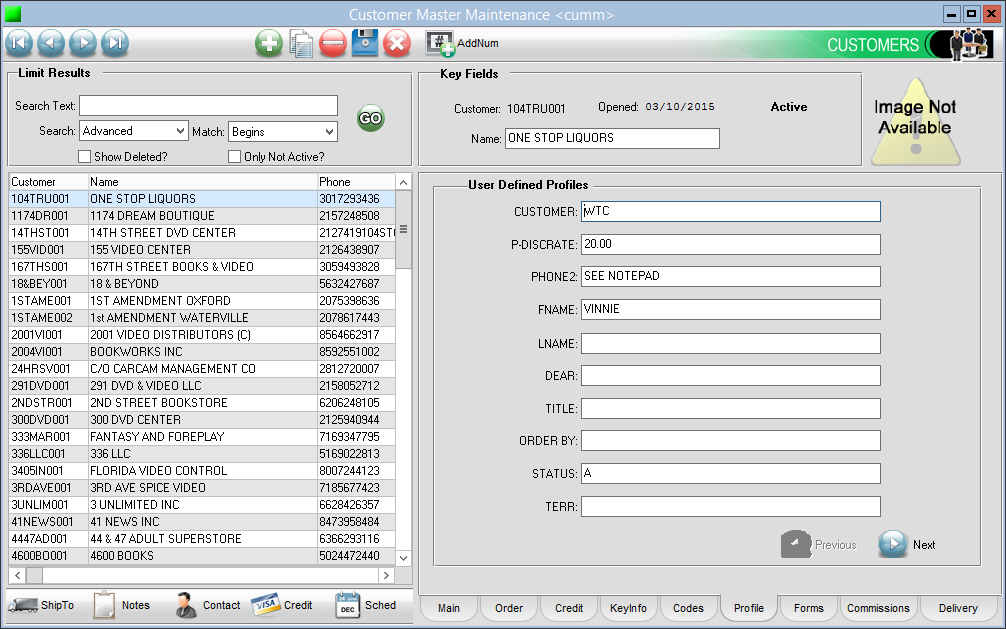
\includegraphics[width=\textwidth]{../img/image80}
		\caption{CUMM Customer Master Maintenance Profile Tab}
	\end{figure}
	
	\item Profile Tab\\
	Sixty additional fields to rename and use any way you want, also available to print on documents.
	
	\begin{figure}[H]
		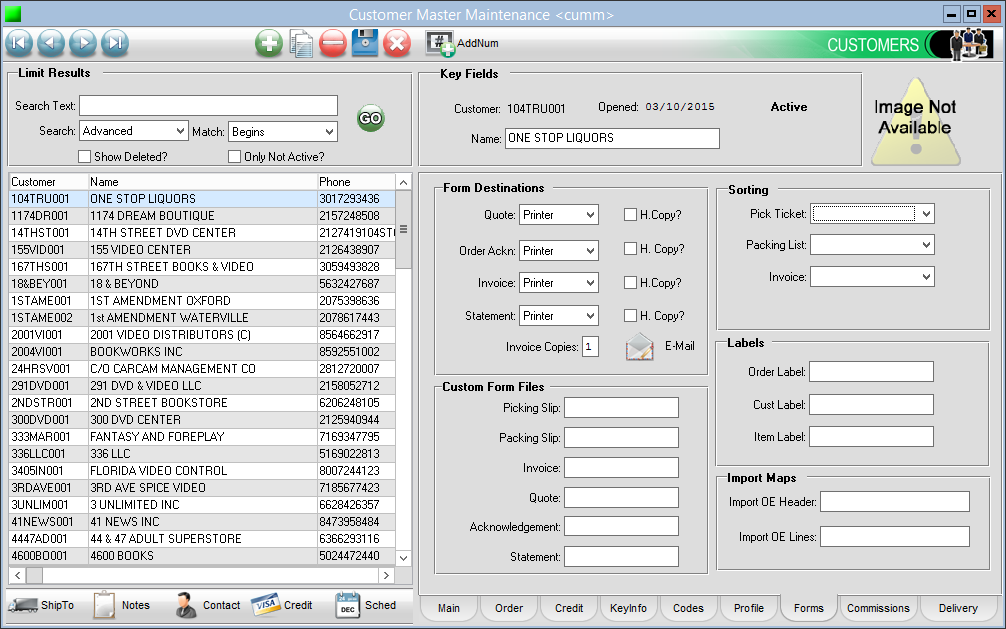
\includegraphics[width=\textwidth]{../img/image81}
		\caption{CUMM Customer Master Maintenance Forms Tab}
	\end{figure}
	
	\item Forms Tab
	\begin{itemize}
		\item Forms Destination \textemdash Set up the defaults on how the forms will be printed, emailed, or faxed to the customers
		\begin{itemize}
			\item Select option for the form
			\item Click Fax / Email Source to choose form
			\item H. Copy \textemdash If checked, hard copy will also be printed
		\end{itemize}
		\item Customer Forms \textemdash If a customer requires a different layout on their forms from the default, the alternative layout can be specified here
		\item Sorting \textemdash Choose specific sorting and printing options here
	\end{itemize}	
	
	\begin{figure}[H]
		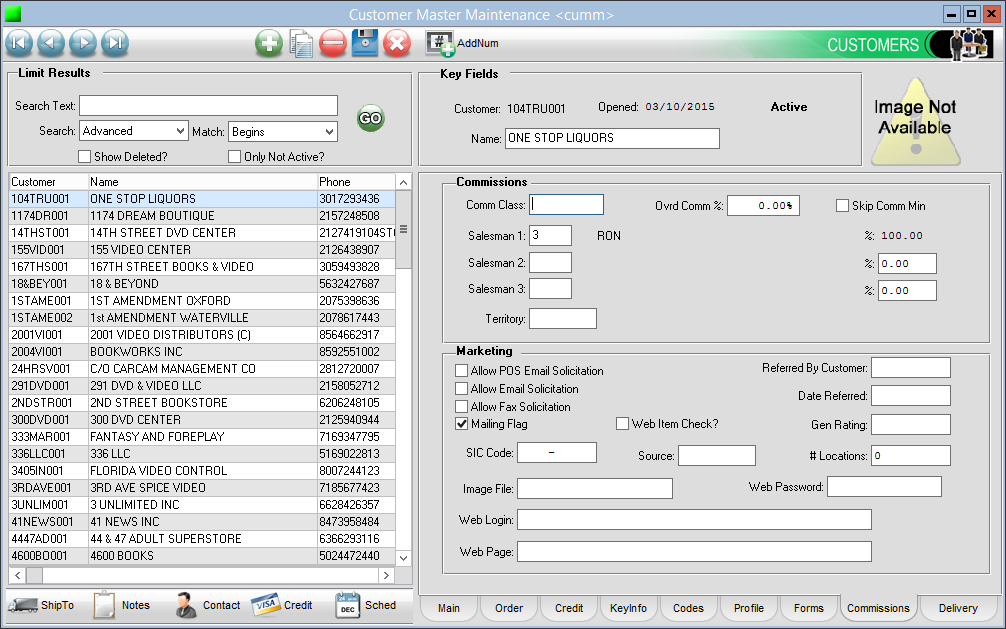
\includegraphics[width=\textwidth]{../img/image82}
		\caption{CUMM Customer Master Maintenance Commissions Tab}
	\end{figure}
	
	\item Commissions Tab
	\begin{itemize}
		\item Salesman 1 \textemdash Using F1 here will allow selecting sales person to receive commissions for this customer
		\item Salesman 2 \textemdash Optional field for split commissions
	\end{itemize}
\end{enumerate}

\subsubsection{Customer Ship To Maintenance}

\index{ERP-One Commands!CUSHM}

The \texttt{CUSHM} command is used to access Customer Ship To Maintenance.

\begin{enumerate}
	
	\begin{figure}[H]
		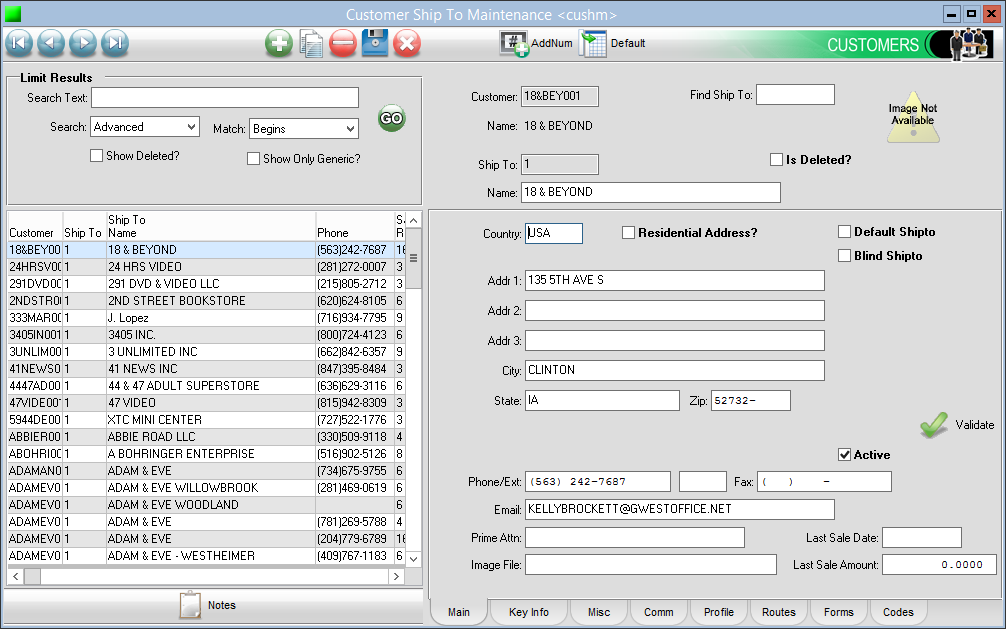
\includegraphics[width=\textwidth]{../img/image83}
		\caption{CUSHM Customer Ship To Maintenance Main Tab}
	\end{figure}
	
	\item Main Tab \textemdash This is where the core data for the customer ship to is stored. If a ship to is not set up that differs from the bill to, the bill to will auto generate into the ship to. Default data can be overridden at order entry time. You can have multiple ship to's.
	\begin{itemize}
		\item Ship to overrides Bill To
		\item Country \textemdash Uses country code, dictates how the address screen is laid out. Using F1 opens selection of country codes.
		\item Address1 \textemdash The address for ship to
		\item Map \textemdash Link to Yahoo! maps
		\item Phone / Fax \textemdash Main numbers for shipping address
		\item Email \textemdash Main email contact for shipping address
		\item Prime Attn \textemdash Primary contact for shipping address
	\end{itemize}
	
	\begin{figure}[H]
		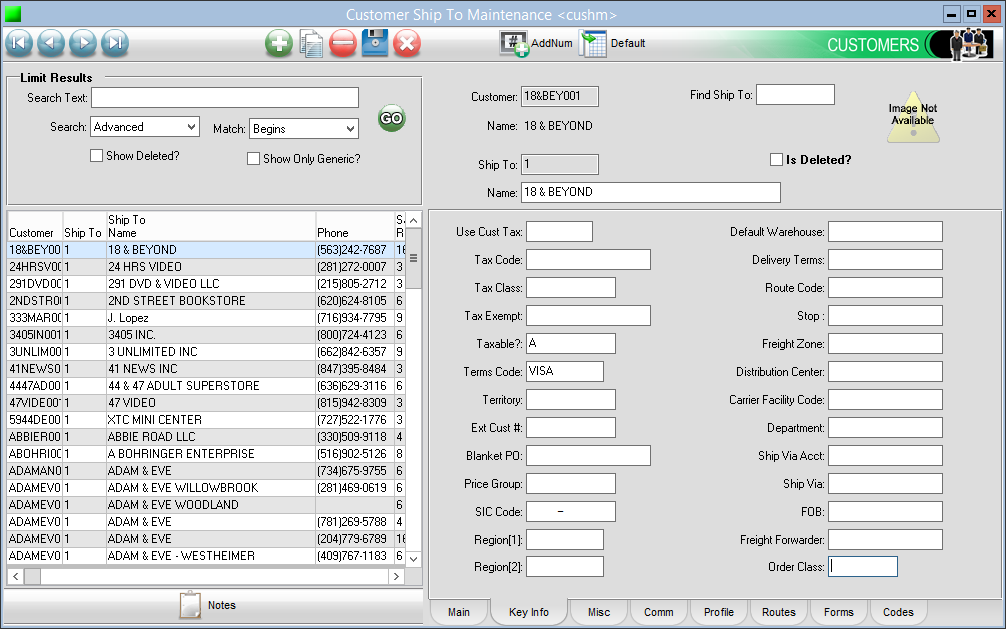
\includegraphics[width=\textwidth]{../img/image84}
		\caption{CUSHM Customer Ship To Maintenance Key Info Tab}
	\end{figure}
	
	\item Key Info Tab\\
	If your shipping terms are different from billing terms, add them here
	\begin{itemize}
		\item Tax
		\item Taxable
		\item Terms
		\item Ship Via
	\end{itemize}
	
	\begin{figure}[H]
		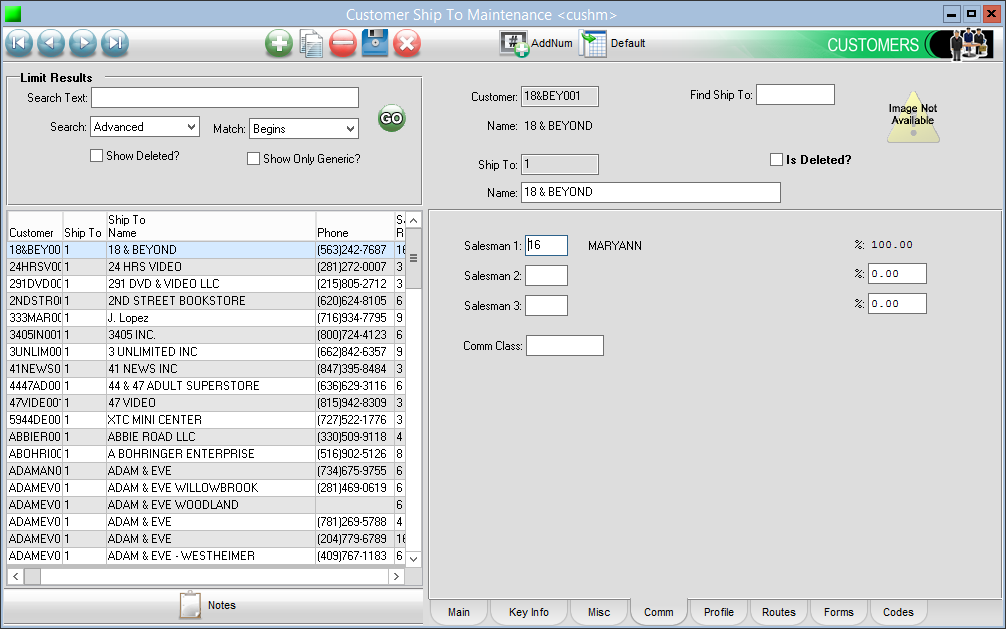
\includegraphics[width=\textwidth]{../img/image85}
		\caption{CUSHM Customer Ship To Maintenance Comm Tab}
	\end{figure}
	
	\item Comm Tab\\
	If commissions are based on ship to address, set up here
	
	\begin{figure}[H]
		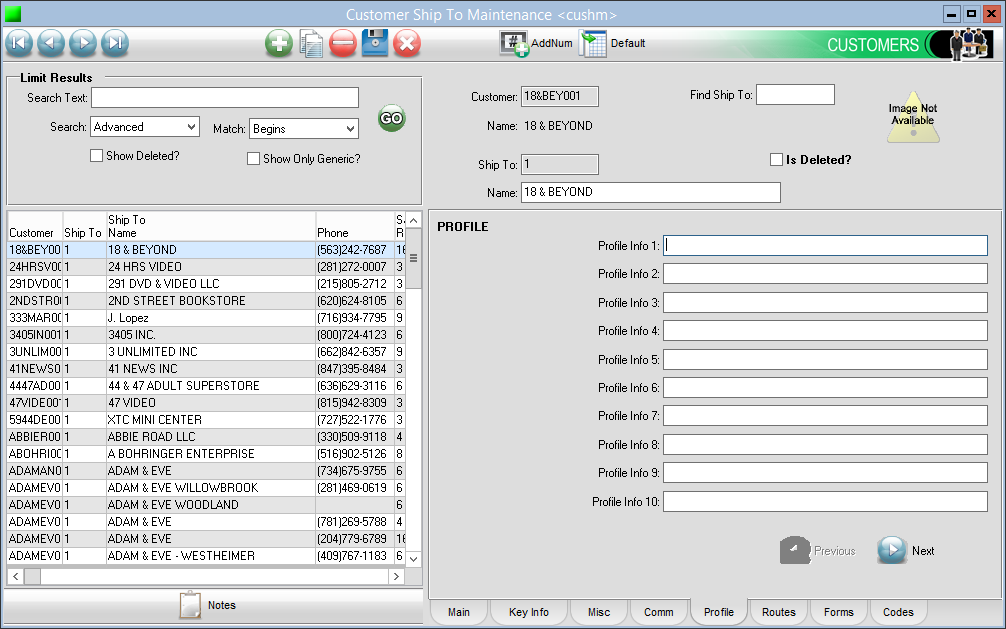
\includegraphics[width=\textwidth]{../img/image86}
		\caption{CUSHM Customer Ship To Maintenance Profile Tab}
	\end{figure}
	
	\item Profile Tab\\
	Sixty additional profile fields to rename and use any way. Option to print on documents.
	
	\begin{figure}[H]
		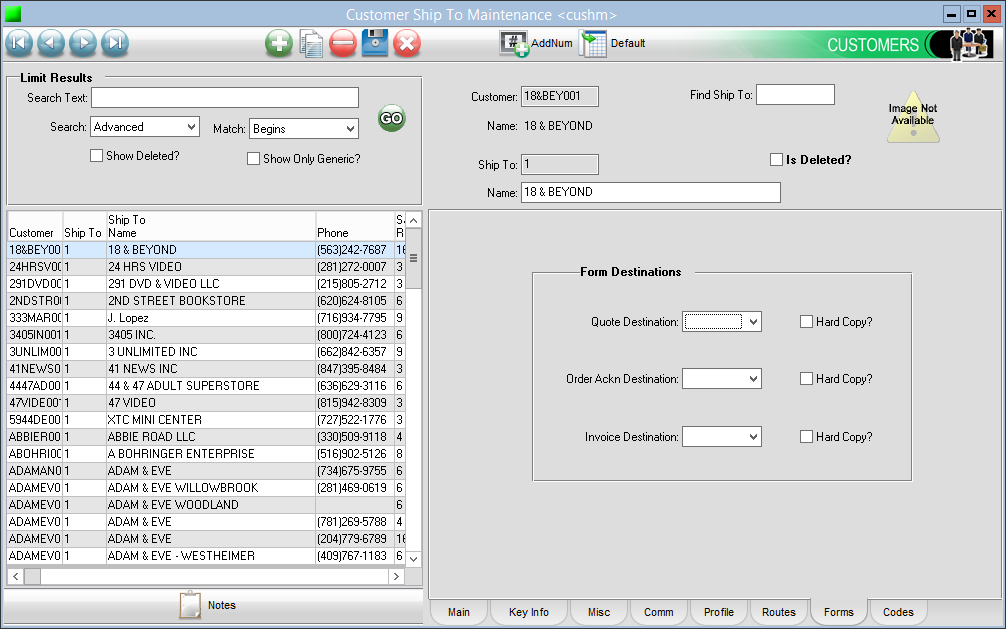
\includegraphics[width=\textwidth]{../img/image87}
		\caption{CUSHM Customer Ship To Maintenance Forms Tab}
	\end{figure}
	
	\item Forms Tab\\
	If you want to define how your forms are printed or sent based on the ship to
	
	\begin{figure}[H]
		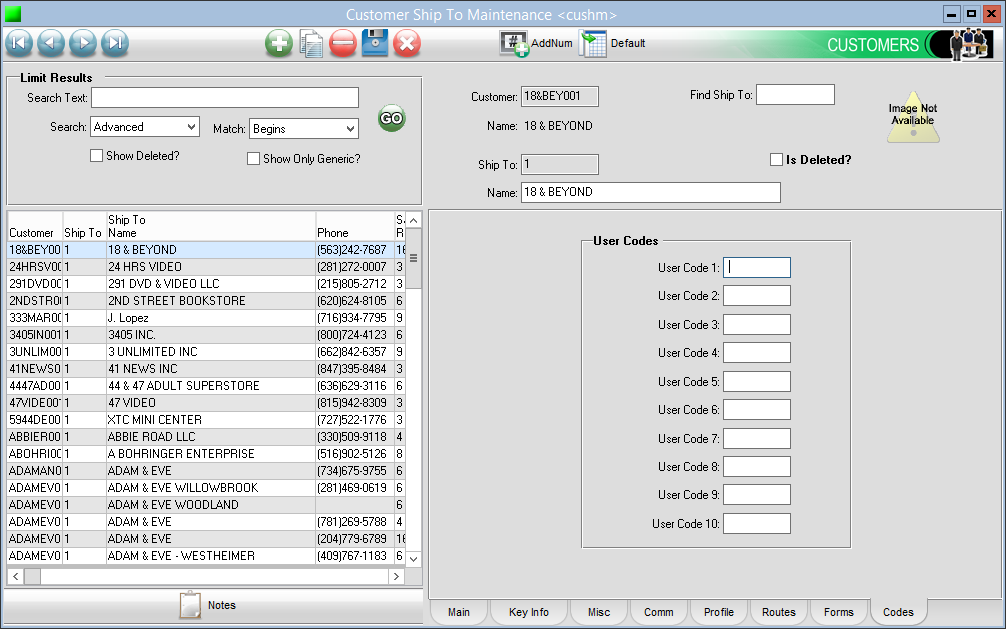
\includegraphics[width=\textwidth]{../img/image88}
		\caption{CUSHM Customer Ship To Maintenance Forms Tab}
	\end{figure}
	
	\item Codes Tab\\
	Ten additional codes to use any way, able to print on documents.
\end{enumerate}

\subsubsection{Customer Notes Maintenance}

\index{ERP-One Commands!CUNM}

The \texttt{CUNM} command is used to access Customer Notes Maintenance.

\begin{figure}[H]
	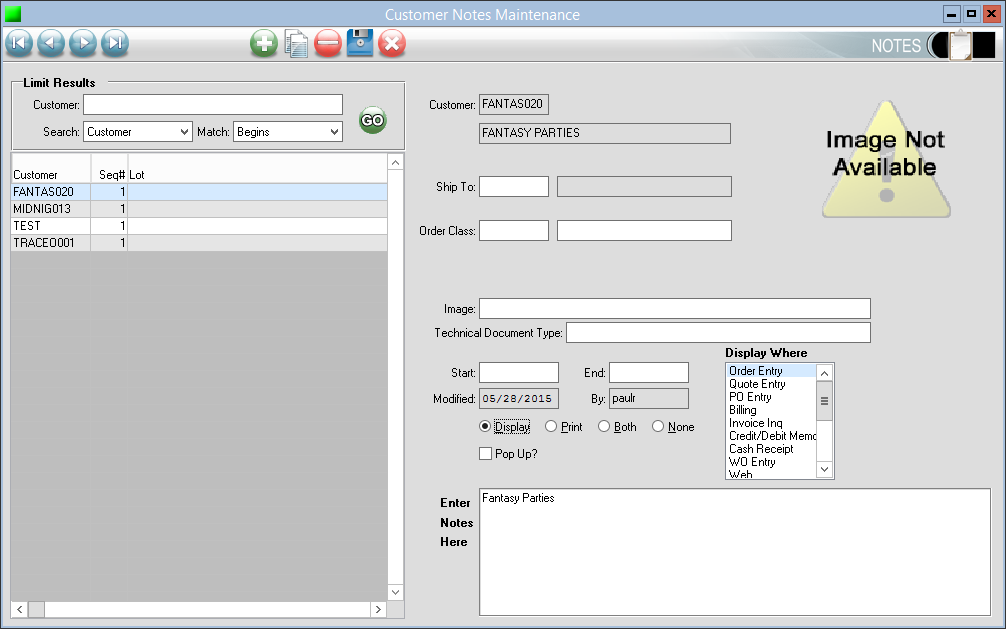
\includegraphics[width=\textwidth]{../img/image89}
	\caption{CUNM Customer Notes Maintenance}
\end{figure}

You can set a note at the customer level. Notes can also be entered at time of order entry per order or line item. Within notes, you have options on there and when to display the note, and what forms you would like it to print on. You can choose for it to be a pop up and / or display, also you may specify an expiration date for when you no longer want that note to be active.

\subsubsection{Customer Contacts Maintenance}

\index{ERP-One Commands!CUCOM}

The \texttt{CUCOM} command is used to access Customer Contacts Maintenance.

\begin{figure}[H]
	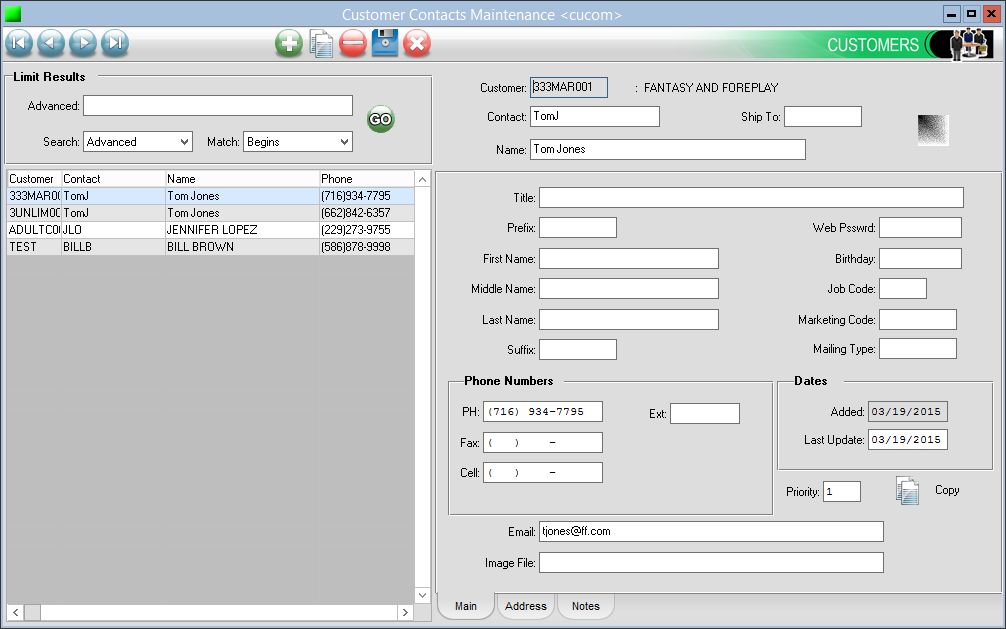
\includegraphics[width=\textwidth]{../img/image90}
	\caption{CUCOM Customer Contacts Maintenance}
\end{figure}

Customer contacts can be added during customer set up as well as during order entry.

\subsubsection{Customer Credit Card Maintenance}

\index{ERP-One Commands!CUCCM}

The \texttt{CUCCM} command is used to access Customer Credit Card Maintenance.

\begin{figure}[H]
	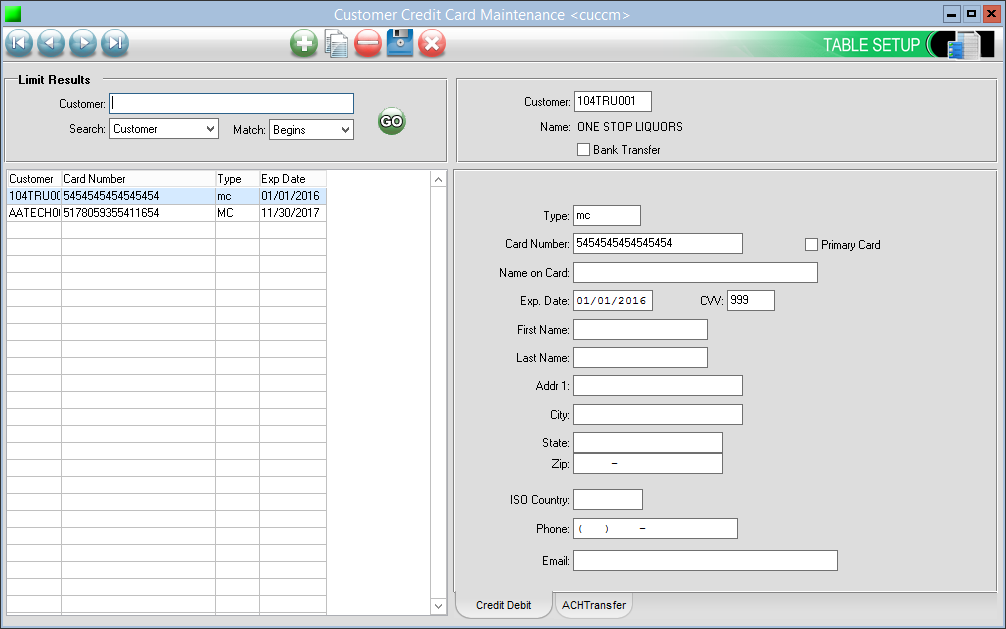
\includegraphics[width=\textwidth]{../img/image91}
	\caption{CUCCM Customer Credit Card Maintenance}
\end{figure}

If a customer pays by credit card for their orders and wants to store their credit card information with you, you may enter it here.

\subsection{Sales Order}

\subsubsection{Sales Order Entry}

\index{ERP-One Commands!OE}

The \texttt{OE} command is used to access Order Entry.

Information on the Order Entry screen will default in, set by the data and required fields you entered in customer setup (\texttt{CUMM}.) You are able to override these fields in order entry.

\begin{enumerate}
	\item Top Buttons
	\begin{itemize}
		\item Accept \textemdash Complete order by clicking \textbf{Accept}, order number will change to permanent order number
		\item Delete \textemdash Delete entire order
		\item Bill Order \textemdash Click \textbf{Bill Order} to process payment
		\item Convert Quote \textemdash Click \textbf{Convert Quote} to convert this order to a quote, you will be prompted with steps to convert to a quote
	\end{itemize}
	
	\begin{figure}[H]
		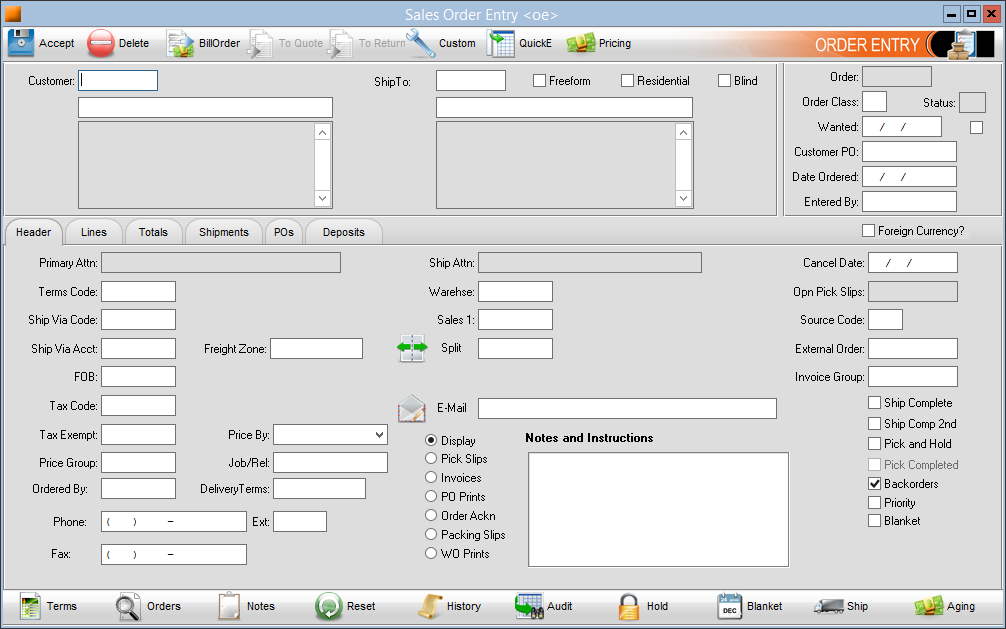
\includegraphics[width=\textwidth]{../img/image92}
		\caption{OE Sales Order Entry Header Tab}
	\end{figure}
	
	\item Header Tab
	\begin{itemize}
		\item Customer \textemdash Customer code, use F1 to search
		\item Ship To \textemdash Use F1 to select Ship To
		\item Address Options
		\begin{itemize}
			\item Freeform \textemdash To add a ship to in order entry, check freeform, add address, then hover over and click on ship to to add as a permanent record
			\item Residential \textemdash Choose residential indicator for shipper
			\item Blind \textemdash Ship blind, packing slip will show customer's ship to address
		\end{itemize}
		\item Order \textemdash Temporary order number will be automatically generated
		\item Order Class \textemdash Required field, default autofilled. Use F1 to open \texttt{OEOCM}
		\item Status \textemdash Status of order:
		\begin{itemize}
			\item CH \textemdash Credit Hold
			\item CL \textemdash Closed
			\item HO \textemdash Order Hold
			\item IV \textemdash Invoice
			\item OE \textemdash Order Entry
		\end{itemize}
		\item Wanted \textemdash Date the customer expects order delivered
		\item Customer PO \textemdash If PO is required, you must enter customer PO number
		\item Date Ordered \textemdash Current date auto-populates, use F1 to open calendar
		\item Entered By \textemdash Defaults to current user
		\item Terms Code \textemdash Required field, use F1 to open \texttt{SYTCM}
		\item Ship Via Code \textemdash Use F1 to open \texttt{SYSVM}
		\item Ship Via Acct \textemdash Enter customer shipping account if required
		\item Tax Code \textemdash Required field, use F1 to open \texttt{CUTXM}
		\item Ordered By \textemdash Customer contact, or use F1 to open list of alternate contacts for customer. Add new contact by hovering over Ordered By and click button that appears
		\item Warehse \textemdash Required field, autofills or use F1 to open \texttt{WAM}
		\item Sales 1 \textemdash Required field, use F1 to open \texttt{CUSRM}
		\item Source Code \textemdash Used to determine how the order was obtained.
		\item External Order \textemdash Web order number
		\item Check Boxes
		\begin{itemize}
			\item Ship Complete \textemdash Items will be allocated from stock, but order will not print until it can be filled 100\%
			\item Ship Comp $2^{nd}$ \textemdash Items in stock will print on first pick slip, backordered items will be allocated as they come into stock and second pick slip will be printed when order is 100\% filled.
			\item Pick and Hold \textemdash Items will be allocated, and pick ticket will be printed so that items can be placed into a staging area until the order is 100\% filled.
			\item Backorders \textemdash If checked, items will be backordered and printed on new pick slip as they come into stock.
		\end{itemize}
		\item Terms \textemdash Summary of terms / discounts with customer for this order
		\item Notes \textemdash Notes can be entered at time of order entry, per order or line item
		\item Aging \textemdash Summary of customer aging, indicates current or late payment		
	\end{itemize}
	
	\begin{figure}[H]
		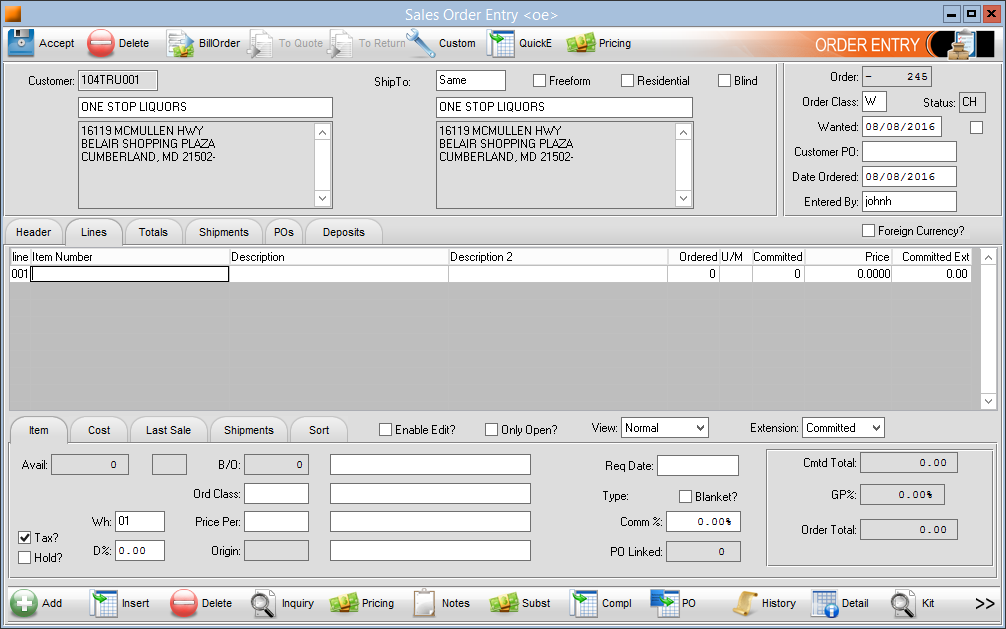
\includegraphics[width=\textwidth]{../img/image93}
		\caption{OE Sales Order Entry Lines Tab}
	\end{figure}
	
	\begin{figure}[H]
		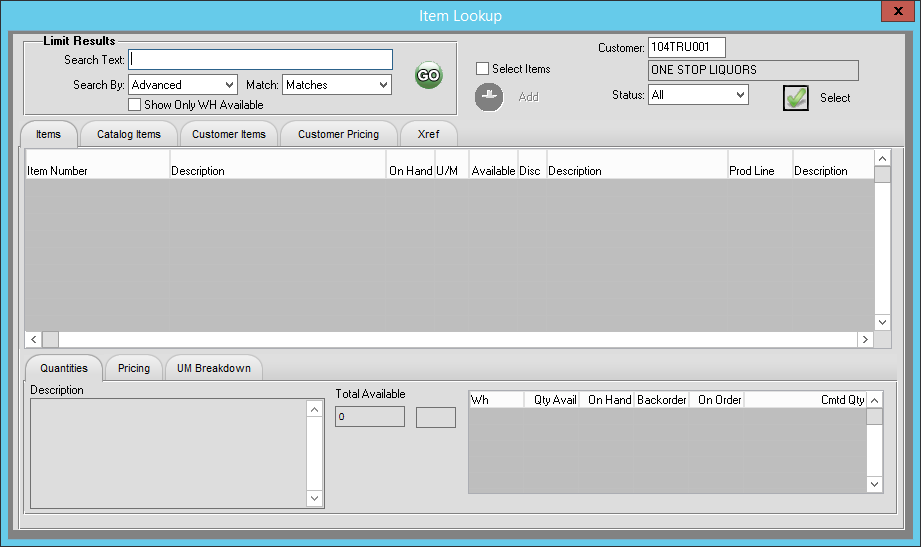
\includegraphics[width=\textwidth]{../img/image94}
		\caption{Product Lookup}
	\end{figure}	
	
	\item Lines Tab
	\begin{itemize}
		\item Line \textemdash Click on \textbf{add} to add line items
		\begin{itemize}		
			\item Item Number \textemdash Enter item number or use F1 to open item search
			\item Description \textemdash Description of item will appear here
		\end{itemize}
		\item Item Tab
		\begin{itemize}
			\item Tax? \textemdash If checked the item is taxable
			\item Wh \textemdash Which warehouse the item is located in
			\item D\% \textemdash Default discount for line item, you are able to add or override discount
			\item PRC \textemdash Order pricing options for gross profit
		\end{itemize}
		\item Cost Tab \textemdash Displays cost of item
		\item Last Sale Tab \textemdash Display price of item last time it was sold to this customer		
	\end{itemize}
	\item Bottom Buttons Under Lines Tab
	\begin{itemize}
		\item Add \textemdash Add line item
		\item Insert \textemdash Insert a new line item between two existing items
		\item Delete \textemdash Delete highlighted line item(s)
		\item Inquiry \textemdash Open \texttt{WAINQ} for highlighted line item
		\item Pricing \textemdash Display pricing information for highlighted line item
		\item Item Notes \textemdash Used to add notes at the line item level
		\item History \textemdash Display customer item purchase history for line item
		\item $\gg$
		\begin{itemize}
			\item Save Options \textemdash Save screen options you have changed for this login
			\item Assembly kit information for line item
			\item Lot and location information for line item
		\end{itemize}
	\end{itemize}
	
	\begin{figure}[H]
		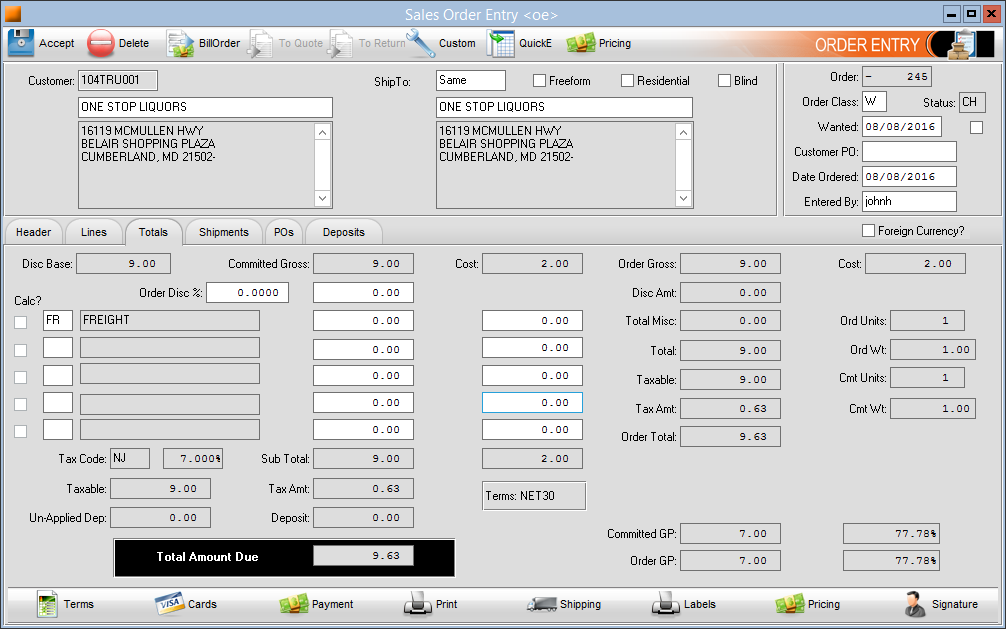
\includegraphics[width=\textwidth]{../img/image95}
		\caption{OE Sales Order Entry Totals Tab}
	\end{figure}	
	
	\item Totals Tab
	\begin{itemize}
		\item Additional Charges \textemdash Using F1 in this field will open \texttt{OETCM} to allow selection of any additional charge types
		\item Tax Code \textemdash Tax code defaults from header screen to this field
		\item Taxable \textemdash Calculated amount of tax
		\item Un-Applied Dep \textemdash Displays deposit paid to be applied to invoice
		\item Total Amount Due \textemdash Total amount due, including shipping, discounts and tax		
	\end{itemize}
	
	\begin{figure}[H]
		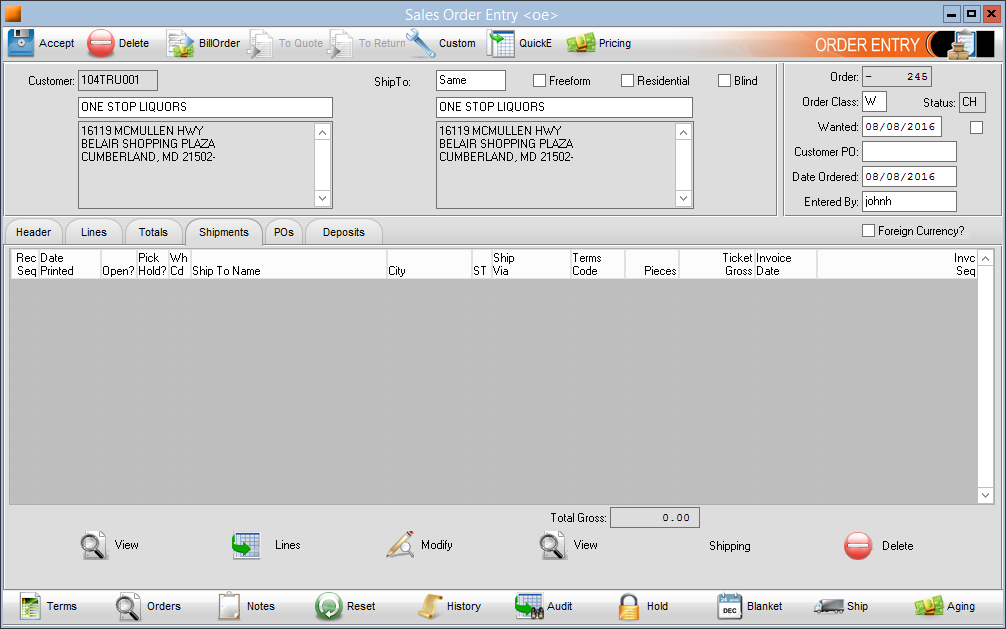
\includegraphics[width=\textwidth]{../img/image96}
		\caption{OE Sales Order Entry Shipments Tab}
	\end{figure}	
	
	\item Shipments Tab
	\begin{itemize}
		\item View Ship \textemdash Opens \texttt{OEIS}
		\item Lines \textemdash Displays lines in shipment
		\item Modify \textemdash Modify shipment
		\item View Inv \textemdash View invoice associated with shipment
		\item Shipping \textemdash Displays tracking and shipping information
		\item Delete \textemdash Deletes shipment record
	\end{itemize}
\end{enumerate}

\subsubsection{Order Lookup and Inquiry}

\index{ERP-One Commands!OEINQ}

The \texttt{OEINQ} command can is used to access Order Lookup and Inquiry

\begin{figure}[H]
	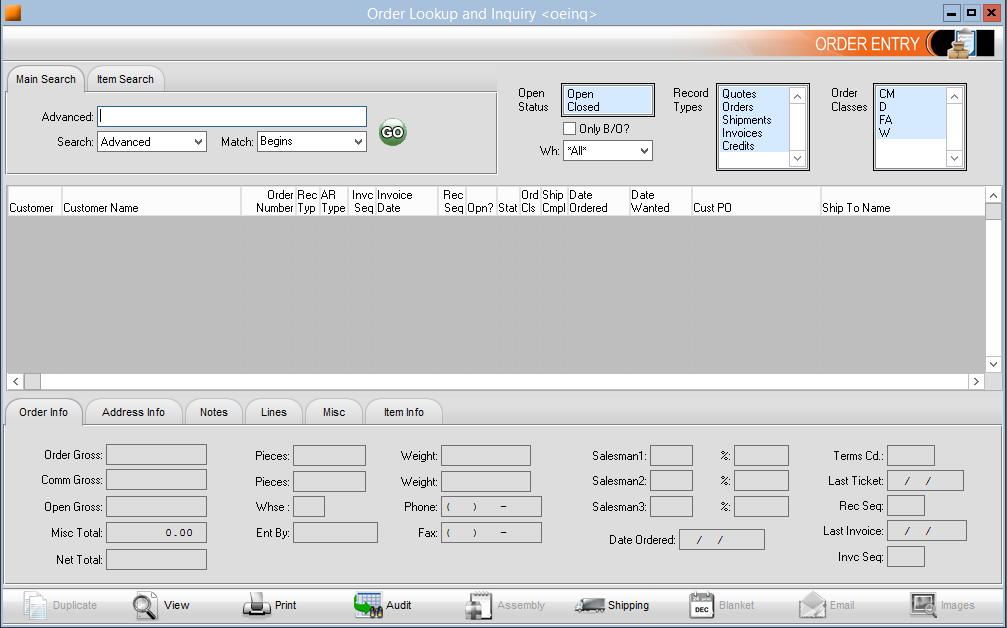
\includegraphics[width=\textwidth]{../img/image5}
	\caption{OEINQ Order Inquiry Screen}
\end{figure}

\begin{itemize}
	\item Open Status \textemdash Search within the status of the order
	\begin{itemize}
		\item Open
		\item Closed
		\item Only B/O? \textemdash If checked, search only orders with backorders
	\end{itemize}
	\item Record Type \textemdash Type of order you want to search through
	\begin{itemize}
		\item Quotes
		\item Orders
		\item Shipments
		\item Invoices
		\item Credits
	\end{itemize}	
	\item Order Class \textemdash Class of order to search, list is managed using \texttt{OEOCM}
	\begin{itemize}
		\item D \textemdash Direct Ship
		\item N \textemdash Rental
		\item W \textemdash From Warehouse
		\item C \textemdash Commission
	\end{itemize}
	\item Results View
	\begin{itemize}
		\item Customer Name
		\item Order Number
		\item Record Type \textemdash An identifier of what type of record is being displayed
		\begin{itemize}
			\item Q \textemdash Quotes
			\item O \textemdash Order
			\item I \textemdash Invoice
			\item S \textemdash Shipment
			\item C \textemdash Credit
		\end{itemize}
		\item Record Sequence \textemdash The number sequence of the document
		\item Invoice Date \textemdash Date Invoices
		\item Order Class
		\item Ship Complete \textemdash Indicates if order was specified to ship complete
		\item Date Ordered
		\item Date Wanted
		\item Cust PO
	\end{itemize}
	\item Bottom Buttons
	\begin{itemize}
		\item View \textemdash View the highlighted order. Opens \texttt{OE} screen for that order.
		\item Print \textemdash Reprint or re-send a document
		\item Audit \textemdash View complete audit for highlighted record
		\item Shipping \textemdash Displays shipment information for order
	\end{itemize}
\end{itemize}

\subsection{Purchase Order}

\subsubsection{Purchase Order Entry}

\index{ERP-One Commands!POE}

The commant \texttt{POE} is used to access Purchase Order Entry.

Information on your purchase order entry screen will auto populate or be filled in by the information entered furing vendor setup in \texttt{VEMM}. The defaulted fields in purchase order entry can be overridden.

\begin{enumerate}
	\item Entry Fields \textemdash Your purchase order will automatically generate a temporary number in the system that will be used until you accept the order.
	\begin{itemize}
		\item Order Class \textemdash Required field. Using F1 opens \texttt{POOCM}
		\item Status \textemdash Status of the order
		\item Date Wanted \textemdash Date you are expecting the order to arrive
		\item Cancel Date \textemdash Date to cancel PO if it has not been received
		\item Date Ordered \textemdash Current date is autofilled. Use F1 to open calendar to choose other date.
		\item Entered By \textemdash Populated with current user id
	\end{itemize}
	\item Top Buttons
	\begin{itemize}
		\item Accept \textemdash Accepts order, temporary purchase order number will be replaced with permanent number
		\item Delete \textemdash Deletes entire order
	\end{itemize}
	
	\begin{figure}[H]
		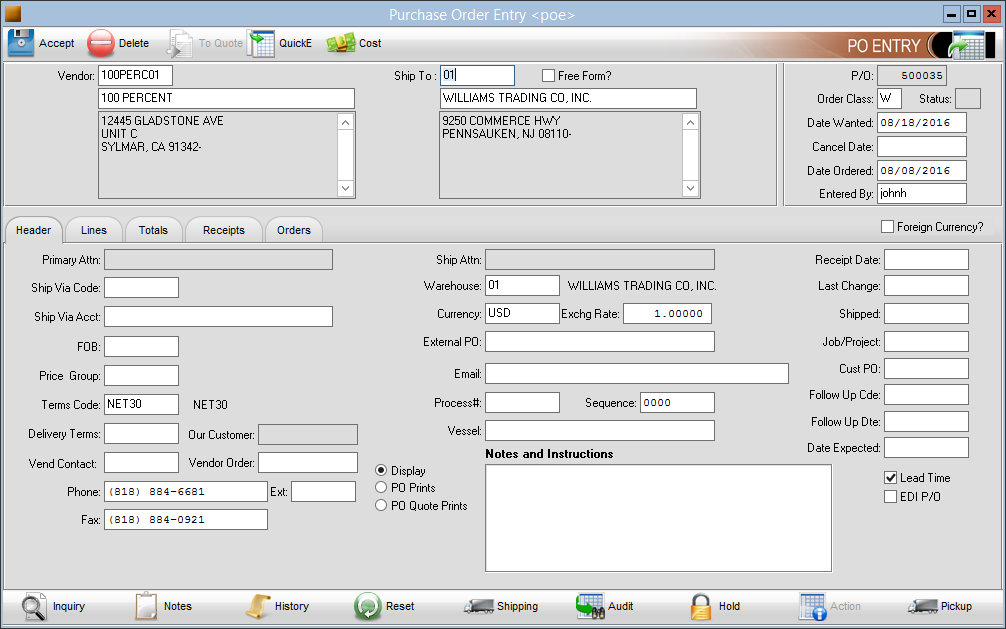
\includegraphics[width=\textwidth]{../img/image97}
		\caption{POE Purchase Order Entry Header Tab}
	\end{figure}
	
	\item Header Tab
	\begin{itemize}
		\item Vendor Field \textemdash Enter vendor code or use F1 to search for vendor.
		\item Ship Via Code \textemdash The shipping method to request for this order, use F1 to open \texttt{SYSVM}
		\item Ship Via Acct \textemdash Optional. The shipping account number to use for shipment.
		\item Terms Code \textemdash Required field. Using F1 opens \texttt{SYTCM}
		\item Warehouse \textemdash Where order is being sent. Using F1 opens \texttt{WAM}	
		\item Follow Up
		\begin{itemize}
			\item Follow Up Code \textemdash Using F1 opens \texttt{POFLOH}
			\item Follow Up Date \textemdash Date to follow up with vendor on status of order if not yet received
			\item Date Expected \textemdash Date of expected delivery of order
		\end{itemize}
		\item Bottom Buttons
		\begin{itemize}
			\item Notes \textemdash Notes can be entered at time of purchase order entry, per order or line item
		\end{itemize}
	\end{itemize}
	
	\begin{figure}[H]
		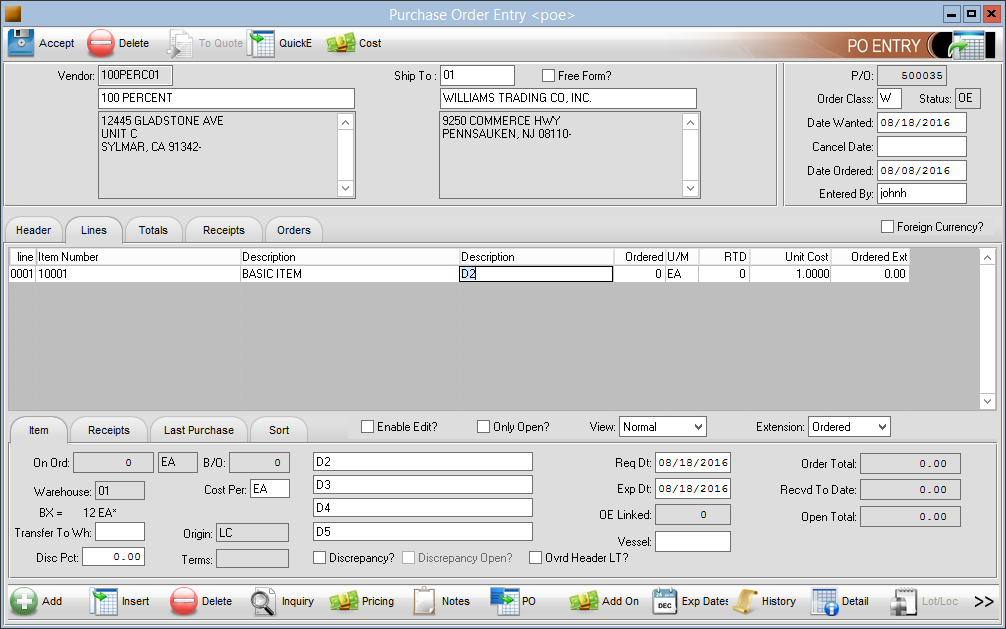
\includegraphics[width=\textwidth]{../img/image98}
		\caption{POE Purchase Order Entry Lines Tab}
	\end{figure}
	
	\item Lines Tab \textemdash Click on the add icon at the bottom to add line items
	\begin{itemize}
		\item Item Number \textemdash Enter item number or use F1 to open item search
		\item Description \textemdash Description of item will appear here
		\item Enable Edit? \textemdash If checked, the cost and other item fields may be modified
	\end{itemize}
	\item Bottom Tabs
	\begin{itemize}
		\item Item
		\begin{itemize}
			\item On Ord \textemdash Quantity of items on all open PO's
			\item Wh \textemdash Warehouse item is located
			\item Disc Pct \textemdash Default discount for line item, able to add or override
			\item B/O \textemdash Quantity on backorder
		\end{itemize}
		\item Cost Per \textemdash Cost per U/M of item
	\end{itemize}
	\item Bottom Buttons
	\begin{itemize}
		\item Add \textemdash Add line item
		\item Insert \textemdash Insert a line item between existing lines
		\item Delete \textemdash Delete selected line item(s)
		\item Inquiry \textemdash Open \texttt{WAINQ} for selected item
		\item Pricing \textemdash Pricing for selected item
		\item Notes \textemdash Add note to selected line item
		\item Exp Date \textemdash Displays expected dates and quantities for line item
		\item $\gg$
		\begin{itemize}
			\item Save Options \textemdash Save screen options you have created
		\end{itemize}
	\end{itemize}
	
	\begin{figure}[H]
		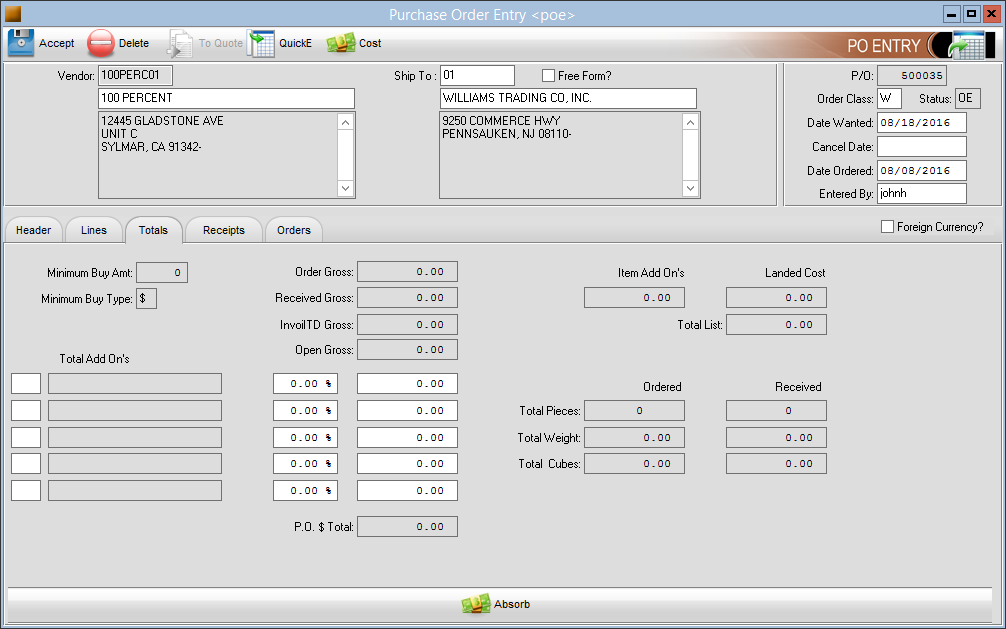
\includegraphics[width=\textwidth]{../img/image99}
		\caption{POE Purchase Order Entry Totals Tab}
	\end{figure}
	
	\item Totals Tab
	\begin{itemize}
		\item Total Add On's / Additional Charges \textemdash Use F1 in this field to open \texttt{POACM} and select any additional charge type
		\item P.O. \$ Total \textemdash Total amount due, including shipping, discounts and tax
	\end{itemize}
\end{enumerate}

\subsubsection{Purchase Order Lookup and Inquiry}

\index{ERP-One Commands!POINQ}

The \texttt{POINQ} command is used to access Purchase Order Lookup and Inquiry.

\begin{figure}[H]
	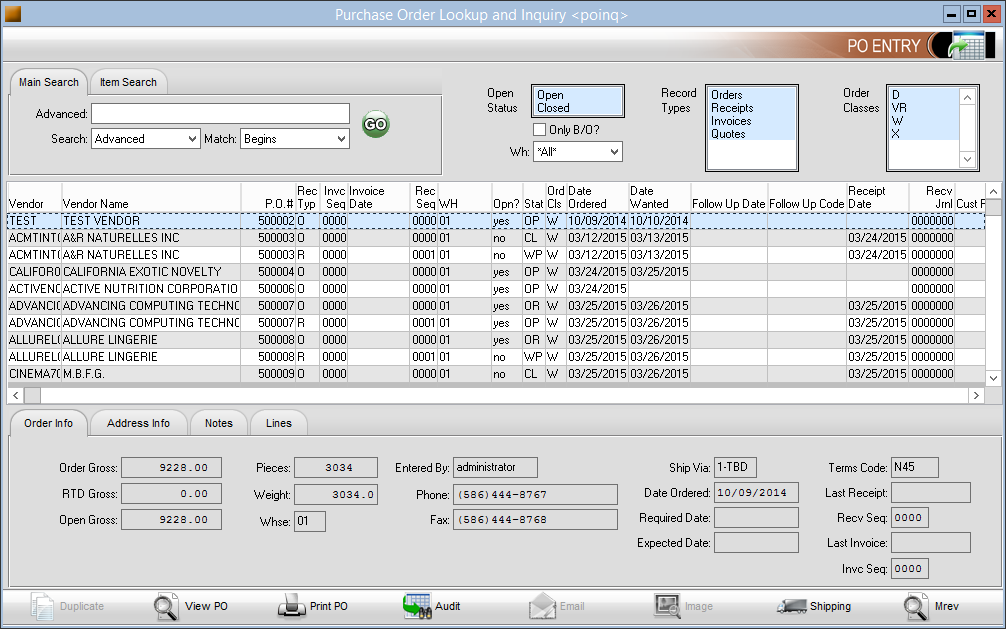
\includegraphics[width=\textwidth]{../img/image100}
	\caption{POINQ Purchase Order Lookup and Inquiry}
\end{figure}

\begin{itemize}
	\item Open Status \textemdash Search within the status of the order
	\begin{itemize}
		\item Open
		\item Closed
	\end{itemize}
	\item Record Type \textemdash Type of order you want to search through
	\begin{itemize}
		\item Quotes
		\item Orders
		\item Invoices
		\item Receipts
	\end{itemize}	
	\item Order Class \textemdash Class of order to search, list is managed using \texttt{OEOCM}
	\begin{itemize}
		\item D \textemdash Direct Ship
		\item W \textemdash From Warehouse
		\item X \textemdash Vendor Returns
	\end{itemize}
	\item Only B/O? \textemdash If checked, search only orders with backorders
	\item Results View
	\begin{itemize}
		\item Vendor Name
		\item Purchase Order Number
		\item Record Type \textemdash An identifier of what type of record is being displayed
		\begin{itemize}
			\item Q \textemdash Quotes
			\item O \textemdash Order
			\item I \textemdash Invoice
			\item R \textemdash Receipts
		\end{itemize}
		\item Record Sequence \textemdash The number sequence of the document
		\item Invoice Date \textemdash Date Invoices
		\item Order Class
		\item Date Ordered
		\item Date Wanted
	\end{itemize}
	\item Bottom Buttons
	\begin{itemize}
		\item View PO \textemdash View the highlighted order. Opens \texttt{POII} screen for that order.
		\item Print \textemdash Reprint or re-send a document
		\item Audit \textemdash View complete audit for highlighted record
	\end{itemize}
\end{itemize}

\subsubsection{Purchase Order Suggested Buy}

\index{ERP-One Commands!POSB}

\begin{figure}[H]
	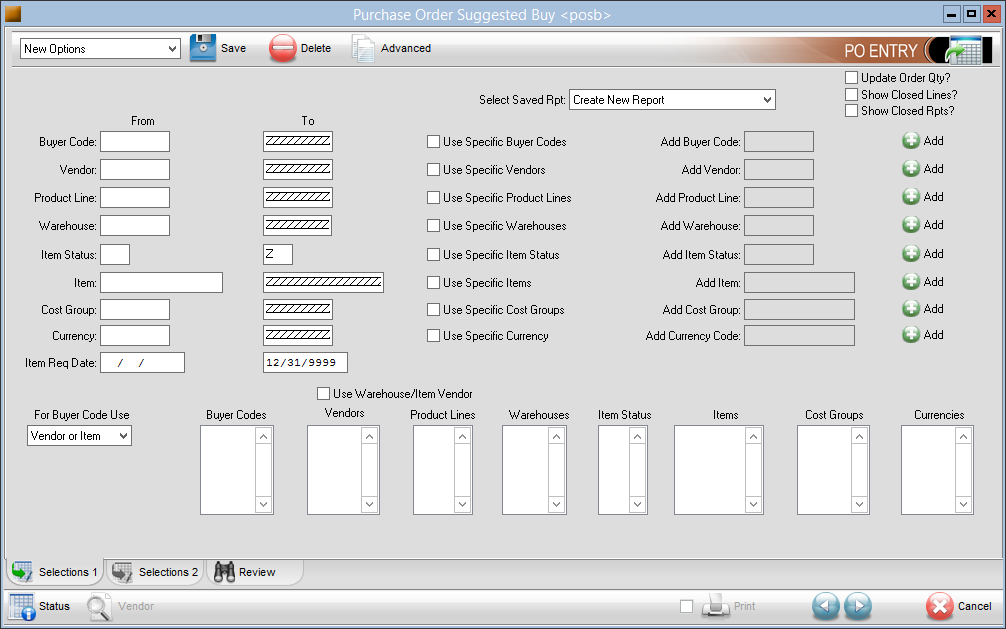
\includegraphics[width=\textwidth]{../img/image101}
	\caption{POSB Purchase Order Suggested Buy}
\end{figure}

\begin{enumerate}
	\item Selections 1 \textemdash This screen allows for the selection of criteria for items that will appear in the review
	\item Selections 2 \textemdash Further options for review
	\item Review \textemdash This will process and show the resulting list of items that need to be purchased
	\begin{itemize}
		\item Vendor List \textemdash This is the default vendor for the item
		\item Item List \textemdash These are the items needed from the highlighted vendor
	\end{itemize}
\end{enumerate}

\subsection{Information Inquiry Reference}

\subsubsection{Inventory Inquiry}

\index{ERP-One Commands!WAINQ}

Looking up information about items in the warehouse may be accomplished using the \texttt{WAINQ} command.

\begin{figure}[H]
	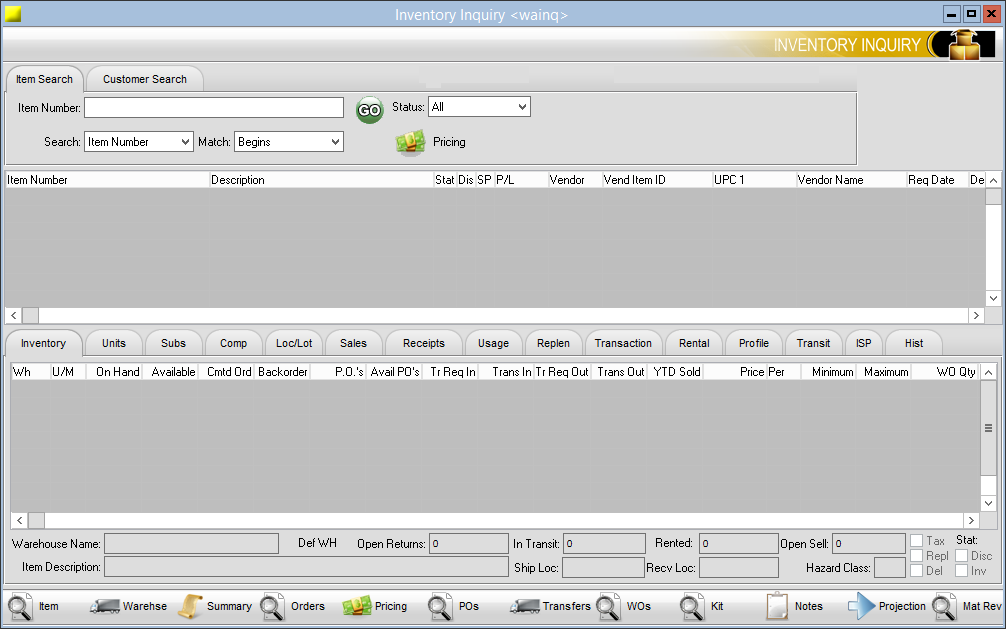
\includegraphics[width=\textwidth]{../img/image53}
	\caption{WAINQ Inventory Inquiry}
\end{figure}

The default search settings will allow you to search for items by their item number. Changing the \textbf{Search} and \textbf{Match} dropdown options will allow you to perform advanced searches for items.

\begin{figure}[H]
	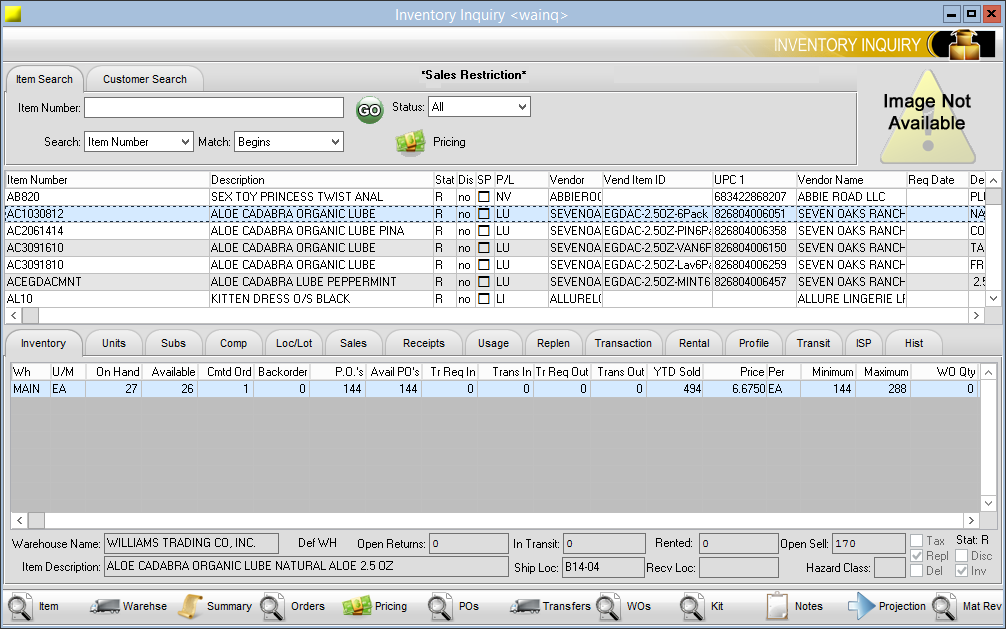
\includegraphics[width=\textwidth]{../img/image54}
	\caption{WAINQ Inventory Inquiry Detail}
\end{figure}

Selecting an item will display detail about that item.

\subsubsection{Order Lookup}

\index{ERP-One Commands!OEINQ}

Looking up information regarding an order that has been entered into the system is straight-forward. The \texttt{OEINQ} command in ERP-ONE will allow you to view the progress of any order and access any documents.

\begin{figure}[H]
	\includegraphics[width=\textwidth]{../img/image5}
	\caption{OEINQ Order Inquiry Screen}
\end{figure}

You may search for an order by the order number, the website order number, the customer's purchase order number, and many more.  Be sure to select 'Advanced' and 'Matches' in the Search and Match drop down boxes if you are having difficulty finding an order without access to the order number.

When you find an order, you may click on it to view the following information:

\begin{figure}[H]
	\includegraphics[width=\textwidth]{../img/image6}
	\caption{OEINQ Order Inquiry Screen with order selected}
\end{figure}

The \textbf{Audit} and \textbf{Shipping} buttons will allow you to view useful information to the customer when providing status updates on their order.

You can also easily access detailed customer information by right clicking on the order, and selecting \textbf{Drill to...} which will give you the option to view the \textbf{Customer Inquiry} and \textbf{Sales History Inquiry} for that customer.

\begin{figure}[H]
	\includegraphics[width=\textwidth]{../img/image7}
	\caption{OEINQ Drill To options}
\end{figure}

\index{ERP-One Commands!CUI}

Selecting \textbf{Customer Inquiry} will direct you to the Customer Inquiry screen that allows you to view the current payment status of the customer.

\begin{figure}[H]
	\includegraphics[width=\textwidth]{../img/image8}
	\caption{CUI Customer Inquiry}
\end{figure}


\section{Warehouse Console}

\subsection{CartonLookup}

CartonLookup can be used to verify the information for a carton that has been collected by the CubiScan device.

\subsection{ItemTracker}

ItemTracker can be used to print out unique ID labels for serializing items, as well as recording their movement out of the building.  This is a preliminary function of the application and has not yet been used in practice. This has no other effect aside from creating a log of which particular item left the building on a specific order.

\subsection{PackerJournal}

PackerJournal can be used to view the performance of individual packers based on their user ID.  This only shows the performance of packers who have used UCC packing methods.

\subsection{PickerJournal}

PickerJournal allows a log to be maintained of who was assigned an order before picking.

\subsection{ProductDimensions}

ProductDimensions allows the lookup of an item's physical dimensions based on information stored on our website catalog.

\subsection{ProductLookup}

ProductLookup provides a quick view of availability counts and bin location for an item.
\chapter{Websites}
\section{MUFFSANDCUFFS.COM}

The MUFFSANDCUFFS.COM website is used by drop-ship customers of Williams Trading Co. to manage their orders. Information is updated regularly in the resources section, and help is available for customers wishing to access our catalog data.

\subsection{General Users}

Any login account has access to browse the catalog. Only customers may view pricing or add items to their cart however. The user's status is determined by options set by the administrator under User Management. A user can either be STANDALONE, which is not attached to any customer account, a customer attached to a single customer number, or an administrator with full access to the site's administrative functionality.

\subsubsection{Browsing the Catalog}

The catalog is arranged by Category and Manufacturer. The item's associated manufacturer is managed from within ERP One, and the categorization is managed through the WHOLESALE.WILLIAMS-TRADING.COM website.

\subsubsection{Searching for Products}

Products can be searched by their item number, or the name of the item. The search is literal, which means no attempt to guess misspellings or like terms is made. Multiple words separated by a space will find items matching all words in any position of the item name. Manufacturer and category names are also 

\subsection{Customers}

\subsubsection{Managing the Cart}

\subsubsection{Submitting an Order}

\subsubsection{Viewing and Managing Orders}

\subsection{Administration}

\subsubsection{Enabling Manufacturers}

\subsubsection{Enabling Product Types}

\subsubsection{Managing Orders}

\subsubsection{Exporting Orders}

\subsubsection{Managing Users}

\section{WILLIAMSTRADINGCO.COM}

\subsection{General Users}

\subsubsection{Browsing the Catalog}

\subsubsection{Searching for Products}

\subsection{Customers}

\subsubsection{Managing the Cart}

\subsubsection{Submitting an Order}

\subsubsection{Viewing and Managing Orders}

\subsection{Administration}

\subsubsection{Enabling Manufacturers}

\subsubsection{Enabling Product Types}

\subsubsection{Managing Orders}

\subsubsection{Exporting Orders}

\subsubsection{Managing Users}

\section{WHOLESALE.WILLIAMS-TRADING.COM}

\subsection{Browsing the Catalog}

\subsection{Editing Products}

\section{COMMANDCENTER.WILLIAMS-TRADING.COM}

\subsection{Managing Promotional Banners}
\chapter{Operations}
\section{Warehouse}

The warehouse is responsible for moving product from receiving to shipping.

\subsection{Picking}

Orders are printed out on demand or in batches and assigned to pickers to be assmbled for the packers.

\subsubsection{Importing Orders}

\index{ERP-One Commands!ORDIMP}

Orders that have been placed through the online order management system must first be imported into ERP-ONE before they can be printed. Perform all the following steps from within the RDP session connected to \textbf{WT-RDS01}

\begin{enumerate}
	\item Login to website
	\item Download orders to import directory
	\item Run \texttt{ORDIMP}
\end{enumerate}

\paragraph{Logging into the website}

Before you can retrieve the orders from the website, you must log in.

\begin{figure}[H]
	\centering
	\begin{subfigure}[b]{0.4\textwidth}
		\includegraphics[width=\textwidth]{../img/image48}
		\caption{{\tiny WILLIAMSTRADINGCO.COM}}
	\end{subfigure}
	~
	\begin{subfigure}[b]{0.4\textwidth}
		\includegraphics[width=\textwidth]{../img/image47}
		\caption{{\tiny MUFFSANDCUFFS.COM}}
	\end{subfigure}
	\caption{Logging into the website}
\end{figure}

\paragraph{Downloading orders to import directory}

After logging in, navigate to \textbf{Administrator} $\rightarrow$ \textbf{Manage Orders} $\rightarrow$ \textbf{Export Orders}


\begin{figure}[H]
	\centering
	\begin{subfigure}[b]{0.4\textwidth}
		\includegraphics[width=\textwidth]{../img/image49}
		\caption{{\tiny WILLIAMSTRADINGCO.COM}}
	\end{subfigure}
	~
	\begin{subfigure}[b]{0.4\textwidth}
		\includegraphics[width=\textwidth]{../img/image50}
		\caption{{\tiny MUFFSANDCUFFS.COM}}
	\end{subfigure}
	\caption{Exporting Orders}
\end{figure}

Right click on the file you wish to download and choose \textbf{"Save Link As..."} if you are in Chrome, or \textbf{"Save Target As..."} in Internet Explorer. A save dialog will open. 

Navigate to the E:{\textbackslash}WEB directory and save the files as \textbf{header.txt} and \textbf{detail.txt}.

If the files already exist, you should first confirm that no one is currently trying to import orders. After you have confirmed that no one else is trying to import orders, you may overwrite the files by clicking on either header.txt or detail.txt and clicking save. If you receive an error regarding permissions you must contact the administrator to have these files removed.

\paragraph{Peforming the import}

After the files have been placed in the correct directory, you may now perform the import by opening \texttt{ORDIMP} and clicking \textbf{Import\textsl{}}.

\begin{figure}[H]
	\centering
	\includegraphics[width=0.5\textwidth]{../img/image46}
	\caption{ORDIMP Import}
\end{figure}\textsl{}

\subsubsection{Printing Pick Lists}

\index{ERP-One Commands!OEPS}

Pick lists are printed using the \texttt{OEPS} command in ERP-ONE

\begin{figure}[H]
	\includegraphics[width=\textwidth]{../img/image1}
	\caption{Selection screen of OEPS}
\end{figure}

Options on the first selection screen allow the warehouse manager to return a limited selection of orders ready to print. The \texttt{Wave By} option may be changed depending on how the orders are to be picked.

\begin{figure}[H]
	\includegraphics[width=\textwidth]{../img/image2}
	\caption{Additional selection screen of OEPS}
\end{figure}

Options on the second selection screen allow further filtering of orders that will appear on the review screen.

\begin{figure}[H]
	\includegraphics[width=\textwidth]{../img/image3}
	\caption{Review screen of OEPS}
\end{figure}

The review screen is where the warehouse manager will choose which orders they wish to print.  This can be done individually or using the \texttt{Select All} button. If further filtering is required clicking \texttt{Advanced} will pull up the following screen.

\textbf{NOTE} Printing a pick list reserves inventory for that order. Do not print pick lists that are not ready to be picked.

\begin{figure}[H]
	\centering
	\includegraphics[width=0.5\textwidth]{../img/image4}
	\caption{Advanced selection screen of OEPS}
\end{figure}

\subsubsection{Picking Orders}

\begin{figure}[H]
	\includegraphics[width=\textwidth]{../img/image51}
	\caption{Warehouse Console Picking Log}
\end{figure}

Before they head into the aisles pickers must first scan their order(s) into the picker management terminal outside of the warehouse management office.  This ensures that accountability is maintained and the picker is known to be responsible for the order they have been assigned.

\pagebreak

\subsection{Packing}

Orders that have been picked from the aisles are delivered to the packing stations in shopping carts or totes containing multiple bins.  Carts may contain multiple orders, or be a part of a larger order.  Each bin in a tote will be a single order.

\index{ERP-One Commands!UCC}

Packers use the \texttt{UCCSS} command to verify items and print out the \emph{UCC} label which is later used for shipping.

\begin{figure}[H]
\includegraphics[width=\textwidth]{../img/image40}
\caption{UCC Scan Shipping}
\end{figure}

\begin{figure}[H]
	\centering
	\includegraphics[width=0.5\textwidth]{../img/image42}
	\caption{UCC Box Label}
\end{figure}

The UCC box label is to be applied to the top of the carton so it can be read by the \textbf{CubiScan}.

\pagebreak

\subsection{Shipping}

Shippers are responsible for scanning the package identifier that has been affixed to the box by the packer.  They will utilize \textbf{ConnectShip}, or alternatively \textbf{Endicia Professional} or \textbf{Worldship} to print the shipping label.

\subsubsection{ConnectShip}

ConnectShip is a complete manifesting / shipping solution. Order and package information is available to ConnectShip from ERP-ONE and the CubiScan database. Packages that have traveled through the conveyor belt will have been weighed and dimensioned. Packages that have not traveled through the belt (i.e. envelopes) will need to be weighed at the shipping terminal.

\begin{figure}[H]
\includegraphics[width=\textwidth]{../img/image43}
\caption{ConnectShip Load Shipment Data}
\end{figure}

ConnectShip is responsible for chosing and printing the appropriate shipping service for each package.  The user is expected to be able to scan the Order ID from the UCC label that was affixed by the packer, and ConnectShip will retreive all necessary information. The user then does a visual confirmation of the options selected and is then able to press \texttt{F12} or use the mouse to click \texttt{Ship}.  The shipping label will print out and they will apply it to the package. In the case of envelopes the envelope must be placed on the scale before the ship button is pressed

\begin{figure}[H]
\includegraphics[width=\textwidth]{../img/image44}
\caption{ConnectShip Order Review and Ship}
\end{figure}

If an exception occurs during processing, the order is to be placed to the side, and the next order is to be shipped.

\pagebreak

\subsection{Receiving}

Receiving is used to update the warehouse with goods received from the vendor on a purchase order. Typically the vendor will send the product to the warehouse with a packing slip which includes an itemized list of the delivery contents. The vendor packing slip is then verified to the product to confirm that it is correct. The product would then be entered into \texttt{PORCV} for receiving. The receiving is a two step process which requires you to enter in the purchase order receipt \texttt{PORCV} and then post or update the inventory to the warehouse using \texttt{WAPOST}

\subsubsection{Inventory Receipts}

\index{ERP-One Commands!PORCV}

The command \texttt{PORCV} is used to access Inventory Receipts.

Enter in the purchase order number, then hit enter on the keyboard. You can also use F1 to look up the purchase order using the search tool.

You will be presented with a dialog box that allows you to select how you are receiving this order.

\begin{itemize}
	\item Item Selection
	\begin{itemize}
		\item Only Open Line Items \textemdash Only open lines on the PO will be listed
		\item All Line Items \textemdash All line times that have and have not been received on this PO will be listed
	\end{itemize}
	\item Default Quantity
	\begin{itemize}
		\item Zero \textemdash Quantity will default to zero
		\item Quantity Open \textemdash Quantity will default to expected amount remaining on PO
	\end{itemize}
\end{itemize}

After making the selection the purchase order will be listed on the screen. You will now need to enter the actual quantity received. If you selected Zero Default Quantity you will need to enter each line, if you chose Quantity Open you will need to verify the values shown.

The quantity still backordered after receipt will be shown in the entry field. If you wish to mark the order complete, simply change the backorder quantity to zero and the purchase order will be marked complete when hitting accept.

If the item is linked to a sales order, you will see, in red, the quantity linked from the receipt to the sales order.

If the item is only located, you will get a popup for assigning location.

\begin{enumerate}
	\item Type in how many you are assigning to that location
	\item If you are receiving to multiple locations, save the first location then click the next button at the top
	\item After you have assigned all quantities, click save then exit the popup	
\end{enumerate}

If the item is lot controlled and located, after entering the received quantity an additional screen will be shown for you to assign the location and lot number.

\begin{enumerate}
	\item Depending on the location type of the item, it may default to the receiving location. If you want to change the location, you can choose from the left side of the screen and click on the location
	\item If it is lot controlled, you will now assign a lot number unless the system is configured to auto assign a lot number
	\item Enter the quantity received against the lot and / or location
	\item Fill in other information as required
	\item Click save at the top of the screen
\end{enumerate}

If you are receiving into multiple locations, enter quantity to be received into the first location along with the lot information, then click save, and click next and repeat until finished.

\textbf{NOTE} You can use F1 in the location field to search for the location.

When you are finished receiving the order, click accept to begin the next receipt and apply the current one.

Bottom Buttons:

\begin{itemize}
	\item Add \textemdash Add additional items to the receipt if they were not on the original PO
	\item Delete \textemdash Delete the item from the receipt, this does not delete the item from the original PO
	\item Print Label \textemdash This will allow you to print a receiving label for what has been received
	\item Notes \textemdash This will allow you to enter item level notes
	\item Inquiry \textemdash Opens \texttt{WAINQ} for highlighted item
	\item Loc / Lot \textemdash If the item is located or lot controlled, this will reopen the Lot / Location information screen
	\item Add On's \textemdash This allows you to add additional costs to the purchase order
	\item Discrepancy \textemdash This will allow you to add a discrepancy to the receipt which is reportable
	\item Cancel \textemdash Cancel the receipt
\end{itemize}

To modify a receipt after it has been created in \texttt{PORCV} you will use \texttt{PORCVM}. This functions like \texttt{PORCV} but allows the modification of accepted receipts before posting.

\textbf{NOTE} If \texttt{XO} option porcv\_auto\_post has been set to 'yes', \texttt{WAPOST} will automatically open after accepting a receipt.

If the option to automatically post is active, you will be presented with the following options:

\begin{itemize}
	\item Run Allocation? \textemdash This will allocate the receipt to any open back orders
	\item Run Allocation from Whse? \textemdash This will also allocate stock found in the warehouse unrelated to this receipt
	\item Print Pick Tickets? \textemdash This allows you to print pick tickets if any back orders can be filled from recepit
	\item Print Post Report? \textemdash This allows you to print a report of what was received with location detail, lot information, etc. If this is checked, you will be prompted to print the post report
\end{itemize}

To print the picking slips, if any shipments were made possible through the new allocations, \texttt{OEPS} automatically opens. Refer to the section on printing picking slips.

\subsubsection{Receiving Reports}

The following reports are used to assist receiving:

\index{ERP-One Commands!PORPT}
\index{ERP-One Commands!RWS}
\index{ERP-One Commands!POREC}

\begin{itemize}
	\item \texttt{PORPT} \textemdash Open purchase order information
	\item \texttt{RWS} \textemdash Prints a receiving worksheet for open purchase orders
	\item \texttt{POREC} \textemdash Received purchase order information
\end{itemize}

\subsubsection{Warehouse Post}

\index{ERP-One Commands!WAPOST}

Items are not received into the warehouse until they have been posted. The \texttt{WAPOST} command allows you to post receipts into inventory.

\begin{itemize}
	\item Selections Tab \textemdash Set the options for the posting here
	\begin{itemize}
		\item Enable PO Receiving \textemdash This pulls all purchase orders that have been received so you can post them the the warehouse
		\item Enable Allocation \textemdash This will allocate the stock to backordered items on sales orders based on the allocation sort order you choose. If this is not checked then the orders will stay in a backorder status until someone commits them directly from \texttt{OE} or \texttt{OECHR}
	\end{itemize}
	\item Review \& Post \textemdash Create the list of receipts to be posted
	\begin{itemize}
		\item Under "Receiving Info" items to be received will be displayed, check items to be posted, or use "Select All" or "DeSel All" to manage the selection
		\item Under "Allocation Info" backorders that will be filled from this receipt will be displayed, check items to be allocated, or use "Select All" or "DeSel All" to manage the selection
		\item The "Inquiry" button located to the left will open \texttt{WAINQ} for the highlighted item
		\item The "History" button located on the bottom will allow you to review previous postings. \texttt{WARUH} may also be used to view warehouse post history.
		\item You may print a report here by clicking the "Print" button, or you can print the report later in \texttt{WARUH} after posting
		\item The "Cancel" button located on the bottom will cancel the transaction before posting occurs
	\end{itemize}
\end{itemize}

When you are ready to post the selected transactions, click "Post" located to the left of the screen.

\subsection{Dimensioning New Items (Cubiscan)}

\index{cubiscan}

When new items arrive in the building, an example of each should be directed to the person who will be responsible for dimensioning the item using the portable Cubiscan.

\subsubsection{Starting the Cubiscan}

\begin{enumerate}
	\item Ensure that the device is plugged in
	\item Ensure that the power inverter is turned on (display will be on)
	\item Turn on PC
	\item Turn on Cubiscan
	\item After the PC has started, open the QMI application
\end{enumerate}

\subsection{Scanning an Item}

\begin{enumerate}
	\item Ensure that the cubiscan is at zero.
	\begin{itemize}
		\item If fluctuating, check for vibrations or wind around the device
		\item If out of zero, clean glass and remove any obstructions, and press Zero on the Cubiscan display
	\end{itemize}
	\item Ensure that the gate is reset to the home position
	\item With the cursor in the item number field, scan the barcode of the item
	\item Place the item on the glass and then move the gate steadily to the other side and back
	\item On the application screen, ensure that the values have been recorded
	\item Press F4 to save data for the item
\end{enumerate}
\section{Purchasing}

Purchasing is responsible for maintaining proper stock levels in the warehouse.  The ERP-ONE system is capable of automatically adjusting reorder points and quantities to meet demand, these values should be trusted, barring any known issues regarding demand or availability of the individual product itself.

Please consult the Vendor Maintenance, Item Maintenance, and Purchase Order sections for more information.
\section{Sales}

The sales department is responsible for customer retention, growth of our customer base and order aquisition.  The sales department includes the sales manager, sales persons, and customer support representatives.


\chapter{Appendix}
\section{Appendix}

\subsection{Passwords}

You may use this section to record passwords for services that you have been given access to.  Writing passwords down outside of this manual is forbidden, and photo-copies may not be made of this page. Sharing passwords, either your own or those given to you for services you manage is forbidden.

\begin{center}
	\renewcommand{\arraystretch}{2}
	\begin{tabularx}{\textwidth}{|p{5cm}|X|X|}
		\hline 
		Service Name & Username & Password \\ 
		\hline 
		&  &  \\ 
		\hline 
		&  &  \\ 
		\hline 
		&  &  \\ 
		\hline 
		&  &  \\ 
		\hline 
		&  &  \\ 
		\hline 
		&  &  \\ 
		\hline 
		&  &  \\ 
		\hline 
		&  &  \\ 
		\hline 
		&  &  \\ 
		\hline 
		&  &  \\ 
		\hline 
		&  &  \\ 
		\hline 
		&  &  \\ 
		\hline 
		&  &  \\ 
		\hline 
		&  &  \\ 
		\hline 
		&  &  \\ 
		\hline 
		&  &  \\ 
		\hline 
	\end{tabularx} 
\end{center}

\pagebreak

\printindex

\end{document}